\documentclass[a4paper,12pt,oneside]{report}

\usepackage[utf8]{inputenc}
\usepackage[T1]{fontenc}
\usepackage[turkish,shorthands=off]{babel}
\usepackage[top=3cm,bottom=2.5cm,left=3.25cm,right=2.5cm]{geometry}
\usepackage{amsmath,amssymb}
\usepackage{mathptmx}
\usepackage{setspace}
\usepackage{indentfirst}
\usepackage{titlesec}
\usepackage{tocloft}
\usepackage{ragged2e}
\usepackage{graphicx}
\usepackage{float}
\usepackage{chngcntr}
\usepackage{hyperref}

 \def\antet{T.C. \\Fırat Ün\.\i vers\.\i tes\.\i  \\Fen B\.\i l\.\i mler\.\i \:Enst\.\i tüsü}

%----------------------------------------------------------------------------------------
%      TEZ BAŞLIĞI YAZIM ALANI
%----------------------------------------------------------------------------------------

\def\tezbasligi{Strogatz Kitabı Bölüm 6 Çevirisi ve Bölüm Sonu Sorularının Çözümleri}

%\def\tezbasligi{FPGA Tabanlı Genel Amaçlı D\.\i j\.\i tal İk\.\i z S\.\i stem\.\i n\.\i n Gel\.\i şt\.\i r\.\i lmes\.\i \, ve Robot S\.\i mülatörü \.\i le B\.\i rl\.\i kte Kullanılması}
% FPGA Tabanlı Genel Amaçlı Dijital İkiz Sisteminin Geliştirilmesi ve Robot Simülatörü ile Birlikte Kullanımı

% \def\tezbasligien{Design of an FPGA Based Real Time Digital Simulator for Electric Motors and Drive Systems }
\def\tezbasligien{Translation of Strogatz Book Chapter 6 and Solutions to End-of-Chapter Problems}


\def\tezyazari{Selçuk Özdemir}   % kendi adınızı giriniz

\def\derece{Vize Ödevi} % Yüksek Lisans/Doktora Tezi, Seminer Çalışması

\def\dereceen{Midterm Assignment} % Master's Thesis, Ph.D. Thesis veya Seminar Study

\def\abd{\mbox{}}  % bölüm/anabilim dalını gerekirse güncelleyiniz
\def\abden{\mbox{}} % İngilizce Anabilim Dalını Giriniz...

\def\bilimdali{~} %ABD kapsamında bilim dalı var ise doldurunuz 
\def\program{Vize Ödevi}
\def\programen{Midterm Assignment}    % İngilizce Program ismi giriniz  

\def\yil{2026}
\def\ay{Mayıs}
\def\ayen{May}

%----------------------------------------------------------------------------------------------------
%----------------------------------------------------------------------------------------------------
% DANIŞMAN, 2. DANIŞMAN, BAŞKAN ve ÜYE BİLGİLERİNİ GİRİNİZ
% KULLANMADIĞINIZ BÖLÜMLERİ PASİF KONUMA GETİRİNİZ
%----------------------------------------------------------------------------------------------------
%----------------------------------------------------------------------------------------------------

\def\danisman {Prof. Dr. Danışman Adı Soyadı}
\def\danismankurum{Fırat Ün\.\i vers\.\i tes\.\i , Fen \, Fakültes\.\i } 
\def\danismankarar {Onayladım} % Onaylamıyorum

% \def\danismaniki {Unvan Adı SOYADI - yoksa siliniz}
% \def\danismanikikurum{............Üniversitesi, .........Fakültesi} 
% \def\danismanikikarar {Onayladım} % Oynaylamıyorum

\def\baskan {Prof. Dr. Jüri Üyesi 1 Adı Soyadı}
\def\baskankurum{Fırat Ün\.\i vers\.\i tes\.\i , Mühend\.\i sl\.\i k Fakültes\.\i } 
\def\baskankarar {Onayladım} % Oynaylamıyorum

\def\uyebir {Doç. Dr. Jüri Üyesi 2 Adı Soyadı}
\def\uyebirkurum{Fırat Ün\.\i vers\.\i tes\.\i , Mühend\.\i sl\.\i k ve M\.\i marlık Fakültes\.\i }  
\def\uyebirkarar {Onayladım} % Oynaylamıyorum

\def\uyeiki {Doç. Dr. Jüri Üyesi 3 Adı Soyadı}
\def\uyeikikurum{Fırat Ün\.\i vers\.\i tes\.\i , Teknoloj\.\i \, Fakültes\.\i }  
\def\uyeikikarar {Onayladım} % Oynaylamıyorum

\def\uyeuc {Doç. Dr. Jüri Üyesi 4 Adı Soyadı}
\def\uyeuckurum{Fırat Ün\.\i vers\.\i tes\.\i , Mühend\.\i sl\.\i k ve M\.\i marlık Fakültes\.\i } 
\def\uyeuckarar {Onayladım} % Oynaylamıyorum

%\def\uyedort {Unvan Adı SOYADI - yoksa siliniz}
%\def\uyedortkurum{..........Üniversitesi, ......... Fakültes\.\i } 
%\def\uyedortkarar {Onayladım} % Oynaylamıyorum

%\def\uyebes {Unvan Adı SOYADI - yoksa siliniz}
%\def\uyebeskurum{............Üniversitesi, .........Fakültes\.\i } 
%\def\uyebeskarar {Onayladım} % Oynaylamıyorum


\def\sayfasayisi {\normalsize{\pageref{pageromanlst} + \pageref{pagearbclst}}} % Ön Bölüm sayfaları ve tez sayfa sayısı (Özgeçmiş hariçtir) 

\def\itt{06.01.2023} % "23.08.2019" şeklinde giriniz. Tezin Enstitüye ilk teslim edildiği tarih. 
\def\st{14.02.2023} % "23.08.2019" şeklinde giriniz.  


% \def\anahtarkelimeler{Örnek Kelime-1, Örnek Kelime-2, Örnek Kelime-3, Örnek Kelime-4}
\def\anahtarkelimeler{Strogatz, çeviri, doğrusal olmayan dinamikler, bölüm sonu soruları} % Üst satırdaki örneğe göre giriş yapınız.

\def\Keywords{Strogatz, translation, nonlinear dynamics, end-of-chapter problems} % İngilizce Anahtar Kelimeleri giriniz...


\onehalfspacing
\setlength{\parindent}{1cm}
\setlength{\parskip}{0pt}
\hypersetup{hidelinks,hypertexnames=false}

\titleformat{\chapter}[hang]{\Large\bfseries}{\thechapter.}{0.4cm}{\Large\bfseries}
\titleformat{\section}[hang]{\normalsize\bfseries}{\thesection}{0.25cm}{\normalsize\bfseries}
\titleformat{\subsection}[hang]{\small\bfseries}{\thesubsection}{0.2cm}{\small\bfseries}
\titlespacing{\chapter}{0pt}{-0.5cm}{0.8cm}
\titlespacing{\section}{0pt}{0.5cm}{0.25cm}
\titlespacing{\subsection}{0pt}{0.4cm}{0.2cm}

\renewcommand{\contentsname}{İçindekiler}
\renewcommand{\bibname}{Kaynaklar}
\makeatletter
\@addtoreset{figure}{section}
\makeatother
\renewcommand{\thefigure}{\thesection.\arabic{figure}}
\newcommand{\figureplaceholder}[3]{%
\begin{figure}[H]
\centering
\fbox{\parbox[c][4.5cm][c]{0.78\textwidth}{\centering #2\\[0.4cm]\small Görsel dosyası daha sonra \texttt{thesis/images/} klasöründen eklenecektir.}}
\caption{#3}
\label{#1}
\end{figure}
}

\begin{document}

\begin{titlepage}
\begin{center}
\textbf{T.C.}\\
\textbf{Fırat Üniversitesi}\\
\textbf{Fen Bilimleri Enstitüsü}

\vspace{3cm}

{\Large\bfseries \tezbasligi}

\vspace{2cm}

{\large \tezyazari}

\vspace{1cm}

{\large \derece}

\vfill

\ay\ \yil\\
Elazığ
\end{center}
\end{titlepage}

\pagenumbering{roman}
\tableofcontents
\newpage

\pagenumbering{arabic}
\chapter*{Giriş}
\phantomsection
\addcontentsline{toc}{chapter}{Giriş}

\begin{justify}
Bu çalışma, Steven H. Strogatz'ın kitabında yer alan Bölüm 6'nın Türkçeye çevrilmesi ve bölüm sonu sorularının çözümlerinin hazırlanması amacıyla düzenlenmiştir. Bu aşamada yalnızca 6.1 başlıklı \textit{Phase Portraits} kısmı çevrilmiş ve belgeye eklenmiştir.

Çeviride kaynak metnin anlamına bağlı kalınmış; ancak Türkçe akademik anlatım, açıklık ve okunabilirlik gözetilmiştir. Matematiksel ifadeler LaTeX biçiminde yeniden yazılmıştır.
\end{justify}

\newpage

\setcounter{chapter}{5}
\chapter{Faz Düzlemi}

\section{Faz Portreleri}

\begin{justify}
Faz düzlemindeki bir vektör alanının genel biçimi
\begin{align}
\dot{x}_1 &= f_1(x_1,x_2),\\
\dot{x}_2 &= f_2(x_1,x_2),
\end{align}
şeklindedir. Burada $f_1$ ve $f_2$ verilen fonksiyonlardır. Bu sistem, vektör gösterimiyle daha kısa biçimde
\begin{equation}
\dot{\mathbf{x}}=\mathbf{f}(\mathbf{x})
\end{equation}
olarak yazılabilir. Burada $\mathbf{x}=(x_1,x_2)$ ve $\mathbf{f}(\mathbf{x})=(f_1(\mathbf{x}),f_2(\mathbf{x}))$ olur. $\mathbf{x}$ faz düzlemindeki bir noktayı, $\dot{\mathbf{x}}$ ise bu noktadaki hız vektörünü temsil eder. Vektör alanı boyunca hareket eden bir faz noktası, faz düzleminde ilerleyen bir yörüngeye karşılık gelen $\mathbf{x}(t)$ çözümünü çizer (Şekil~\ref{fig:6-1-1}). Ayrıca faz düzleminin tamamı yörüngelerle doludur; çünkü her nokta bir başlangıç koşulu olarak alınabilir.

\begin{figure}[H]
\centering
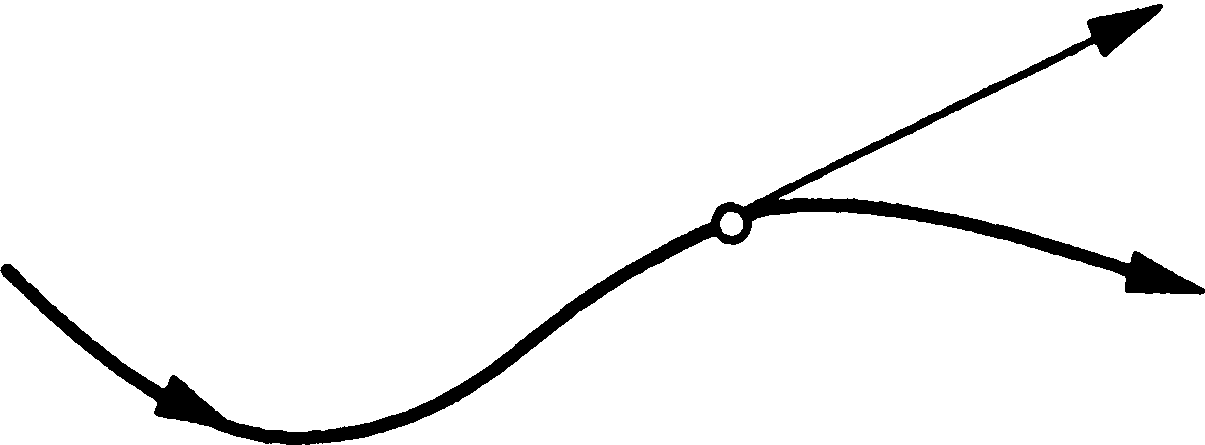
\includegraphics[width=0.82\textwidth]{images/Figures/figur-002.png}
\caption{Faz düzleminde bir yörüngenin gösterimi.}
\label{fig:6-1-1}
\end{figure}

Doğrusal olmayan sistemlerde yörüngeleri analitik olarak bulmak çoğu zaman mümkün değildir. Açık formüller elde edilebildiği durumlarda bile bu formüller genellikle anlamlı bir kavrayış sağlayamayacak kadar karmaşık olur. Bu nedenle çözümlerin nitel davranışını belirlemeye çalışacağız. Amacımız, sistemin faz portresini doğrudan $\mathbf{f}(\mathbf{x})$ fonksiyonunun özelliklerinden çıkarmaktır. Çok çeşitli faz portreleri ortaya çıkabilir; bunun bir örneği Şekil~\ref{fig:6-1-2}'de gösterilecektir.

\begin{figure}[H]
\centering
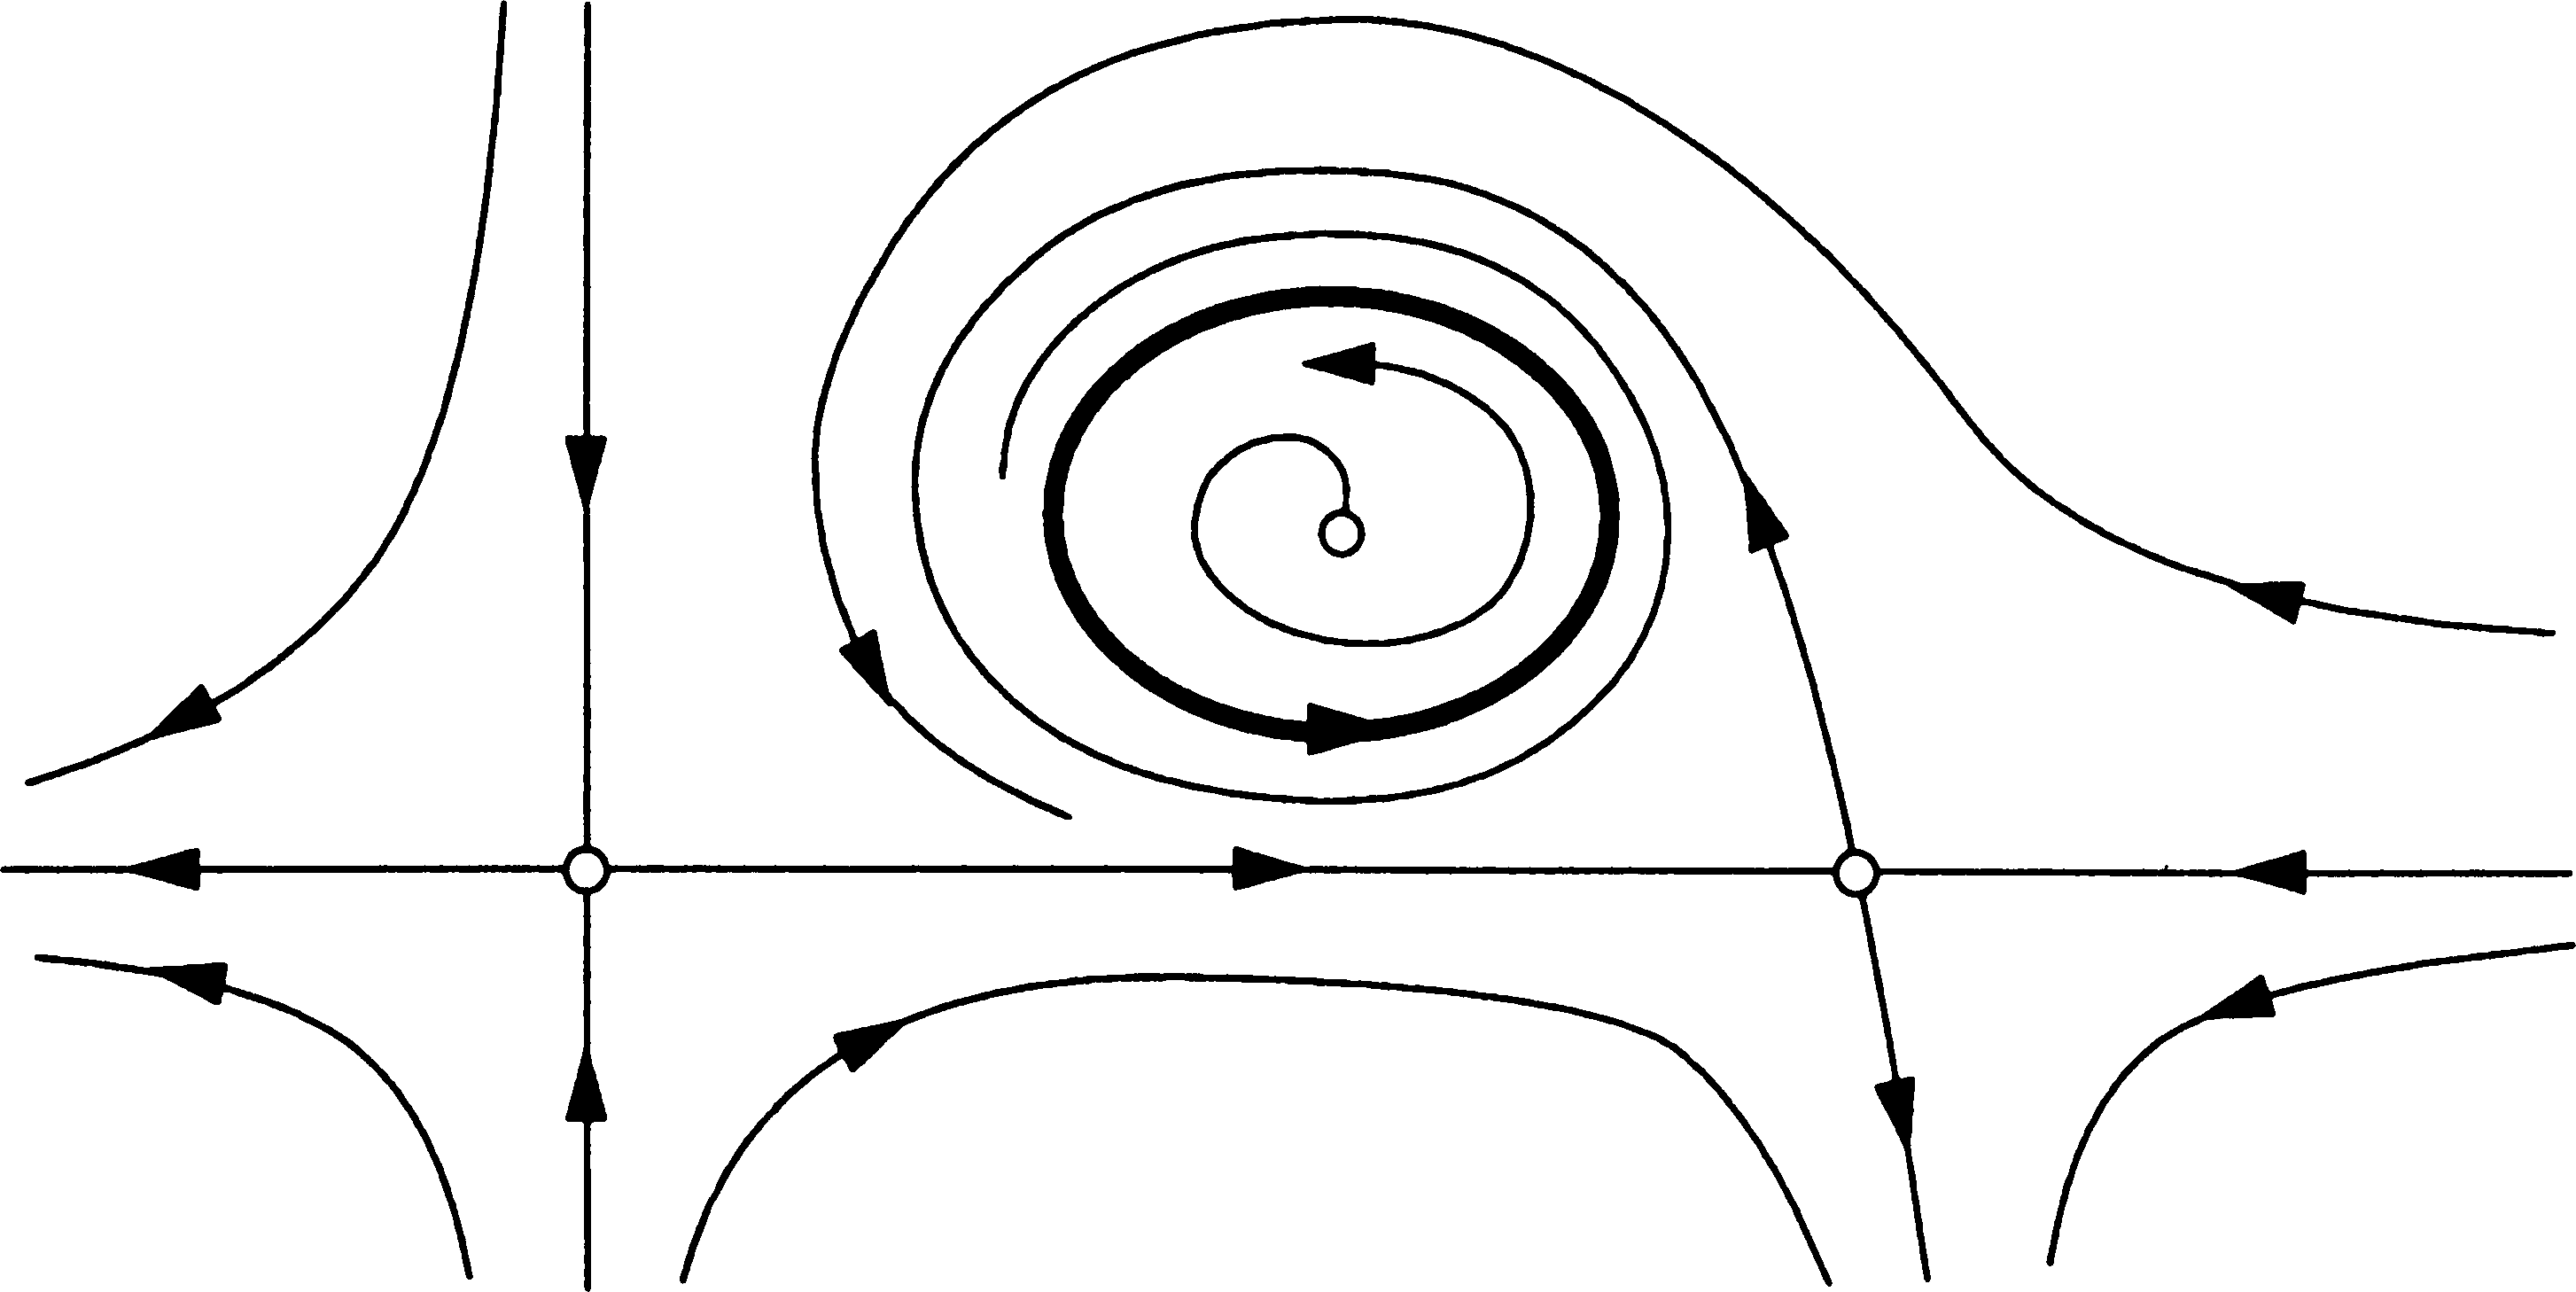
\includegraphics[width=0.82\textwidth]{images/Figures/figur-001.png}
\caption{Sabit noktalar ve kapalı yörünge içeren örnek faz portresi.}
\label{fig:6-1-2}
\end{figure}

Herhangi bir faz portresinin en belirgin özelliklerinden bazıları şunlardır:
\begin{enumerate}
\item \textbf{Sabit noktalar:} Şekil~\ref{fig:6-1-2}'deki $A$, $B$ ve $C$ gibi noktalar sabit noktalardır. Sabit noktalar $\mathbf{f}(\mathbf{x}^{*})=0$ koşulunu sağlar ve sistemin kararlı durumlarına ya da dengelerine karşılık gelir.
\item \textbf{Kapalı yörüngeler:} Şekil~\ref{fig:6-1-2}'deki $D$ gibi kapalı eğriler periyodik çözümleri temsil eder. Başka bir deyişle, bir $T>0$ değeri için tüm $t$ değerlerinde
\begin{equation}
\mathbf{x}(t+T)=\mathbf{x}(t)
\end{equation}
koşulu sağlanır.
\item \textbf{Yörüngelerin yerleşimi:} Sabit noktaların ve kapalı yörüngelerin yakınındaki yörünge düzeni önemlidir. Örneğin $A$ ve $C$ yakınındaki akış deseni birbirine benzerken, $B$ yakınındaki desenden farklıdır.
\item \textbf{Kararlılık ya da kararsızlık:} Sabit noktaların ve kapalı yörüngelerin kararlı olup olmadığı faz portresinin temel özelliklerindendir. Örneğin $A$, $B$ ve $C$ sabit noktaları kararsızdır; çünkü yakınlarındaki yörüngeler bu noktalardan uzaklaşma eğilimindedir. Buna karşılık $D$ kapalı yörüngesi kararlıdır.
\end{enumerate}
\end{justify}

\subsection*{Faz Portrelerinin Sayısal Hesaplanması}
\phantomsection
\addcontentsline{toc}{subsection}{Faz Portrelerinin Sayısal Hesaplanması}

\begin{justify}
Bazı durumlarda faz portresinin nicel özellikleriyle de ilgileniriz. Neyse ki $\dot{\mathbf{x}}=\mathbf{f}(\mathbf{x})$ sisteminin sayısal integrasyonu, tek değişkenli $\dot{x}=f(x)$ denkleminin sayısal integrasyonundan çok daha zor değildir. Önceki sayısal yöntemler, $x$ ve $f(x)$ sayıları yerine $\mathbf{x}$ ve $\mathbf{f}(\mathbf{x})$ vektörleri kullanıldığında yine geçerlidir.

Bu çalışmada Runge--Kutta yöntemi kullanılacaktır. Yöntemin vektörel biçimi
\begin{equation}
\mathbf{x}_{n+1}=\mathbf{x}_n+\frac{1}{6}\left(\mathbf{k}_1+2\mathbf{k}_2+2\mathbf{k}_3+\mathbf{k}_4\right)
\end{equation}
şeklindedir. Burada
\begin{align}
\mathbf{k}_1 &= \Delta t\,\mathbf{f}(\mathbf{x}_n),\\
\mathbf{k}_2 &= \Delta t\,\mathbf{f}\left(\mathbf{x}_n+\frac{1}{2}\mathbf{k}_1\right),\\
\mathbf{k}_3 &= \Delta t\,\mathbf{f}\left(\mathbf{x}_n+\frac{1}{2}\mathbf{k}_2\right),\\
\mathbf{k}_4 &= \Delta t\,\mathbf{f}\left(\mathbf{x}_n+\mathbf{k}_3\right).
\end{align}
Amaçlarımız için genellikle $\Delta t=0.1$ adım büyüklüğü yeterli doğruluk sağlar.

Faz portresi çizilirken vektör alanındaki temsilî vektörlerden oluşan bir ızgarayı görmek çoğu zaman yararlıdır. Ancak ok uçları ve vektör uzunluklarının farklı olması bu tür çizimleri kalabalıklaştırabilir. Bu nedenle yön alanı çizimi daha açık bir görünüm sağlar: Akışın yerel yönünü göstermek için kısa doğru parçaları kullanılır.
\end{justify}

\subsection*{Örnek 6.1.1}
\phantomsection
\addcontentsline{toc}{subsection}{Örnek 6.1.1}

\begin{justify}
Aşağıdaki sistemi ele alalım:
\begin{align}
\dot{x} &= x+e^{-y},\\
\dot{y} &= -y.
\end{align}
Önce nitel argümanlar kullanarak faz portresi hakkında bilgi elde edelim. Daha sonra bilgisayar yardımıyla yön alanını çizelim. Son olarak Runge--Kutta yöntemini kullanarak birkaç yörünge hesaplayalım ve bunları faz düzleminde gösterelim.

\textbf{Çözüm.} İlk olarak sabit noktaları bulmak için $\dot{x}=0$ ve $\dot{y}=0$ denklemlerini birlikte çözeriz. Tek çözüm
\begin{equation}
(x^{*},y^{*})=(-1,0)
\end{equation}
olarak bulunur.

Bu sabit noktanın kararlılığını belirlemek için $y(t)$ davranışına bakalım. $\dot{y}=-y$ denkleminin çözümü
\begin{equation}
y(t)=y_0e^{-t}
\end{equation}
olduğundan $t\to\infty$ iken $y(t)\to 0$ olur. Dolayısıyla uzun vadede $e^{-y}\to 1$ ve $x$ için denklem yaklaşık olarak
\begin{equation}
\dot{x}=x+1
\end{equation}
haline gelir. Bu denklem üstel olarak büyüyen çözümlere sahiptir; bu da sabit noktanın kararsız olduğunu düşündürür. Gerçekte, başlangıç koşullarını $x$ ekseni üzerinde seçersek $y_0=0$ olur ve bundan dolayı tüm zamanlar için $y(t)=0$ kalır. Bu durumda $x$ ekseni üzerindeki akış tamamen $\dot{x}=x+1$ denklemi tarafından belirlenir. Bu nedenle sabit nokta kararsızdır.

Faz portresini çizmek için nulklinleri belirlemek yararlıdır. Nulklinler, $\dot{x}=0$ ya da $\dot{y}=0$ koşullarından birinin sağlandığı eğrilerdir. Bu eğriler akışın nerede tamamen yatay veya tamamen düşey olduğunu gösterir (Şekil~\ref{fig:6-1-3}).

Örneğin akış $\dot{y}=0$ olduğu yerlerde yataydır. $\dot{y}=-y$ olduğundan bu durum $y=0$ doğrusu üzerinde gerçekleşir. Bu doğru boyunca $\dot{x}=x+1$ olur. Dolayısıyla $x>-1$ iken akış sağa doğrudur.

Benzer şekilde akış $\dot{x}=x+e^{-y}=0$ olduğu yerlerde düşeydir. Bu koşul
\begin{equation}
x=-e^{-y}
\end{equation}
eğrisini verir. Eğrinin $y>0$ olan üst kısmında akış aşağı yönlüdür; çünkü burada $\dot{y}<0$ olur.

Nulklinler ayrıca düzlemi, $\dot{x}$ ve $\dot{y}$ işaretlerinin farklı değerler aldığı bölgelere ayırır. Şekil~\ref{fig:6-1-3}'te bu bölgelerdeki tipik vektör yönleri gösterilecektir. Bu bilgiler tek başına bile genel akış deseninin anlaşılması için iyi bir başlangıç sağlar.

\begin{figure}[H]
\centering
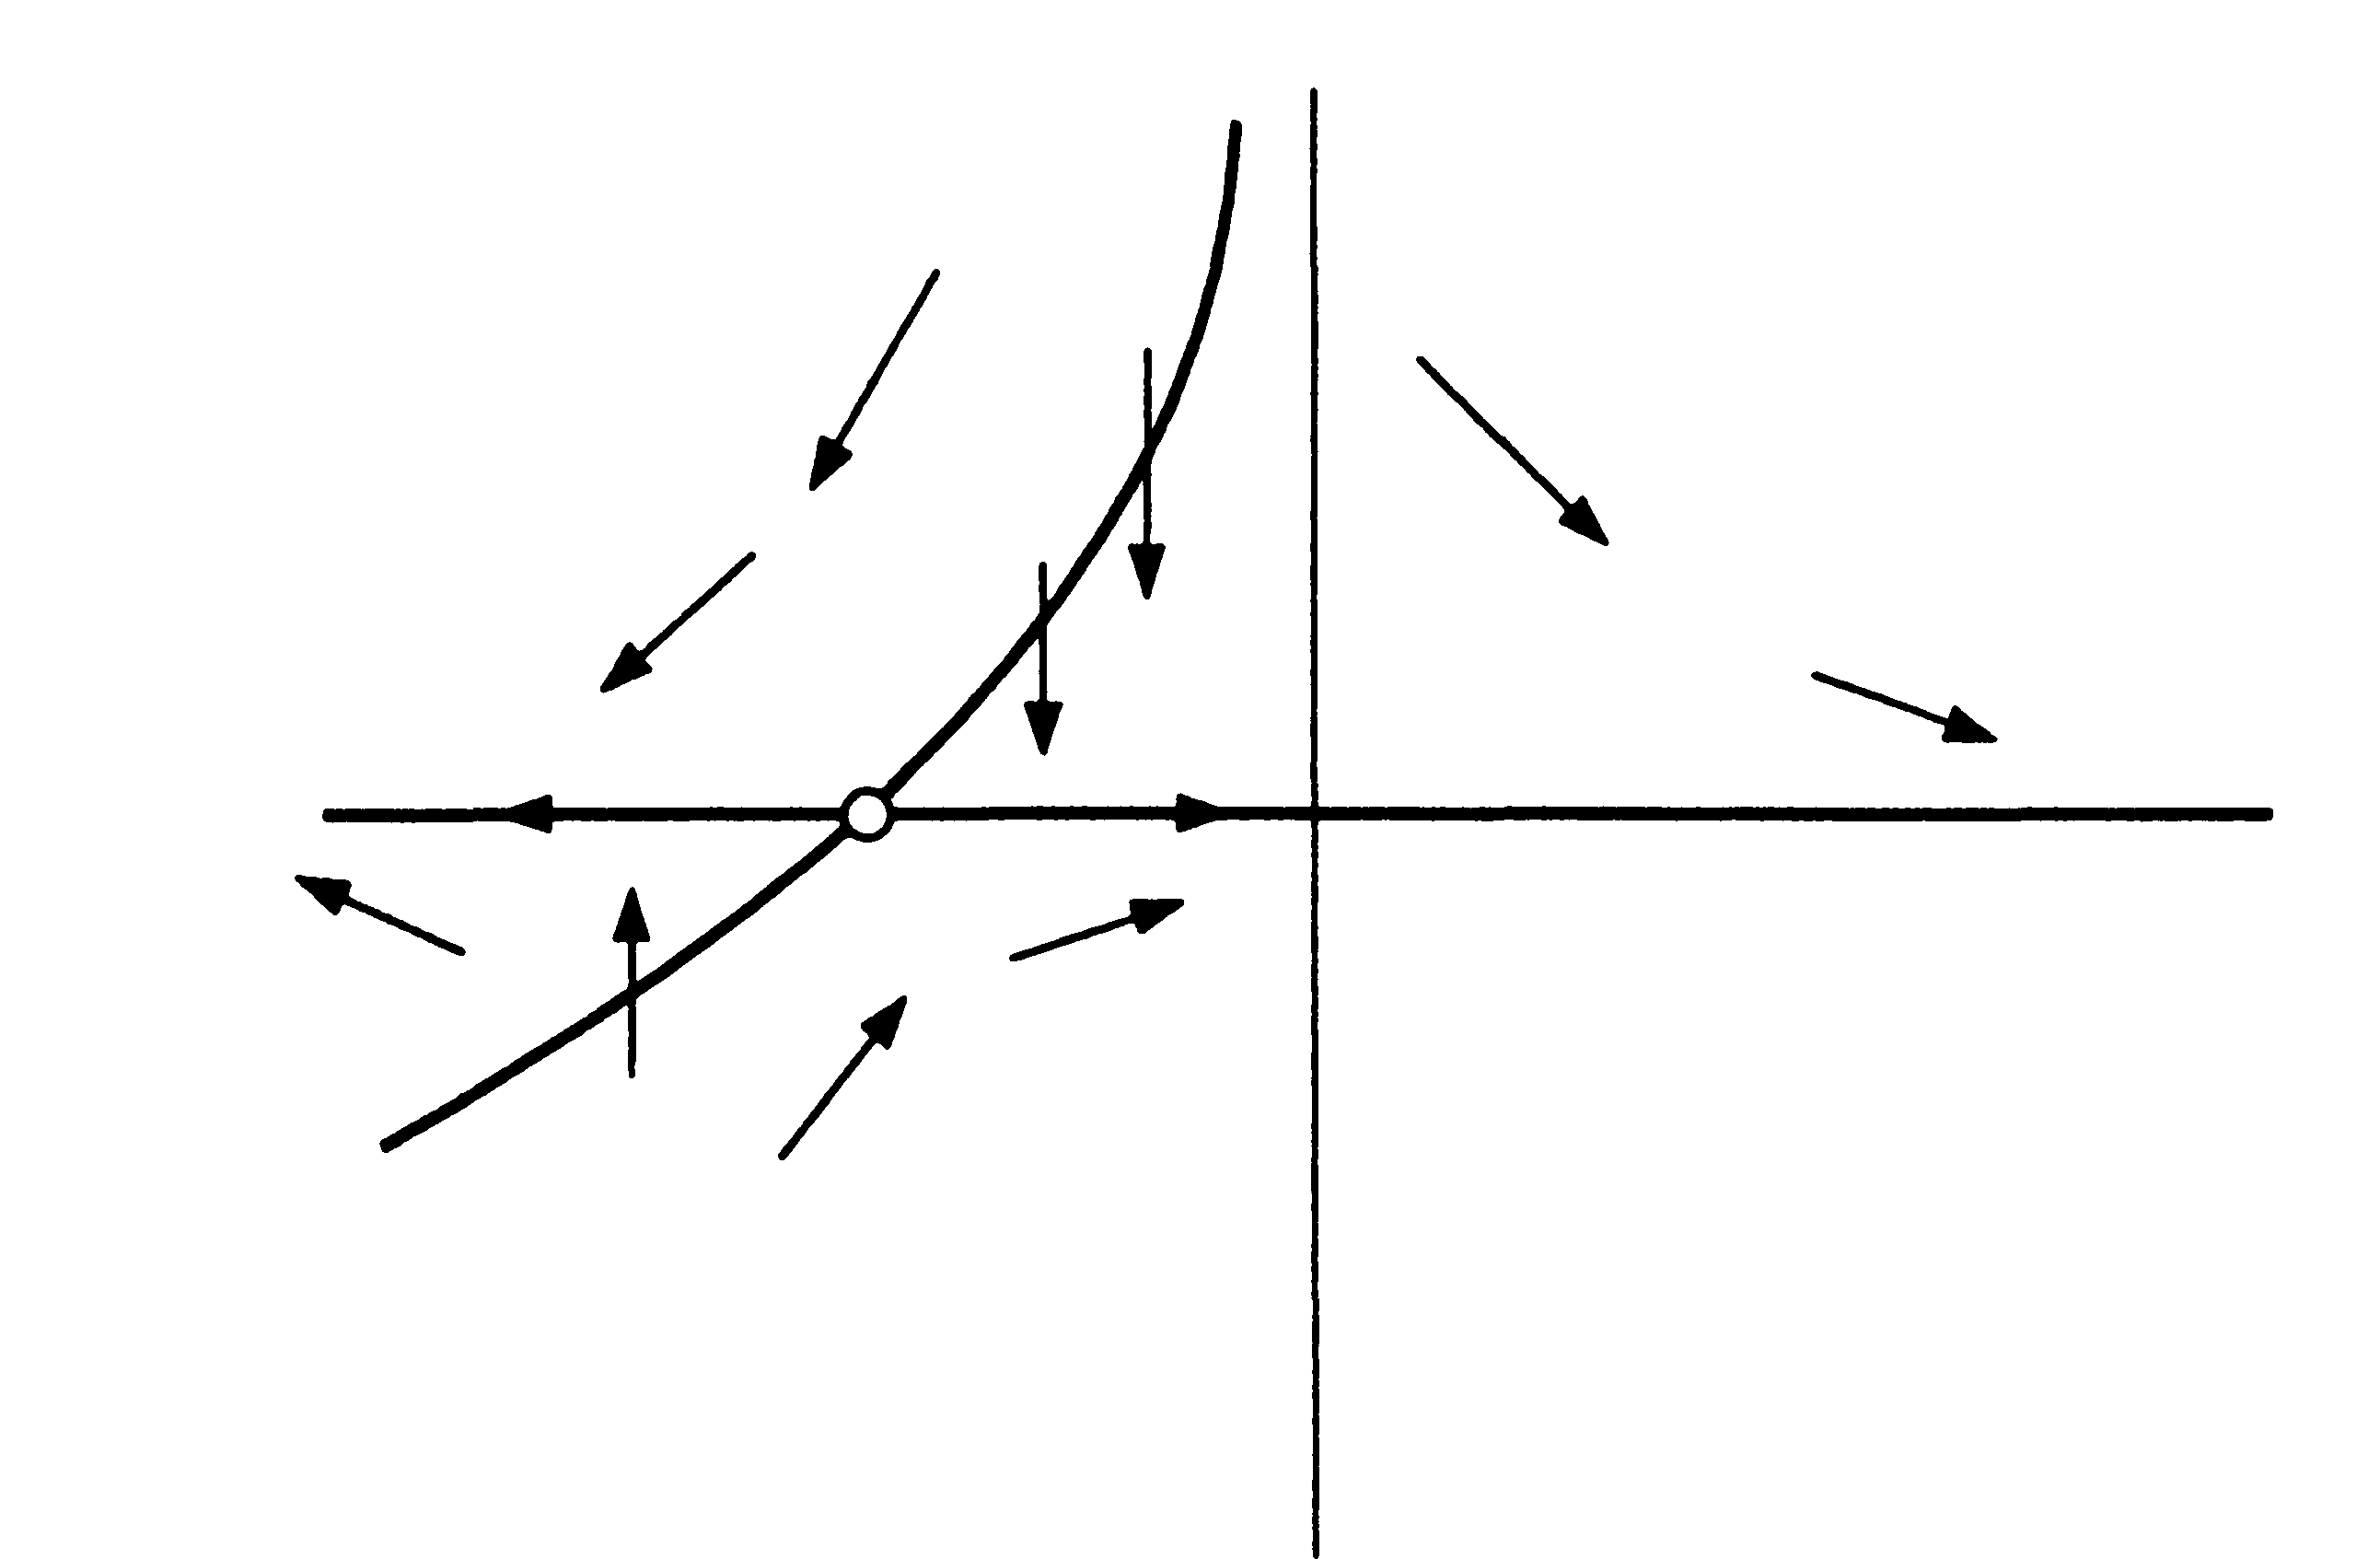
\includegraphics[width=0.82\textwidth]{images/Figures/figur-003.png}
\caption{Örnek 6.1.1 için nulklinler ve bölgelerdeki akış yönleri.}
\label{fig:6-1-3}
\end{figure}

Şimdi problemi tamamlamak için bilgisayar kullanılır. Şekil~\ref{fig:6-1-4}'te yön alanı kısa doğru parçalarıyla gösterilecek ve birkaç yörünge çizilecektir. Yörüngelerin her noktada yerel eğimi izlediği görülür. Böylece sabit noktanın, doğrusal olmayan bir eyer noktası türü olduğu anlaşılır.

\begin{figure}[H]
\centering
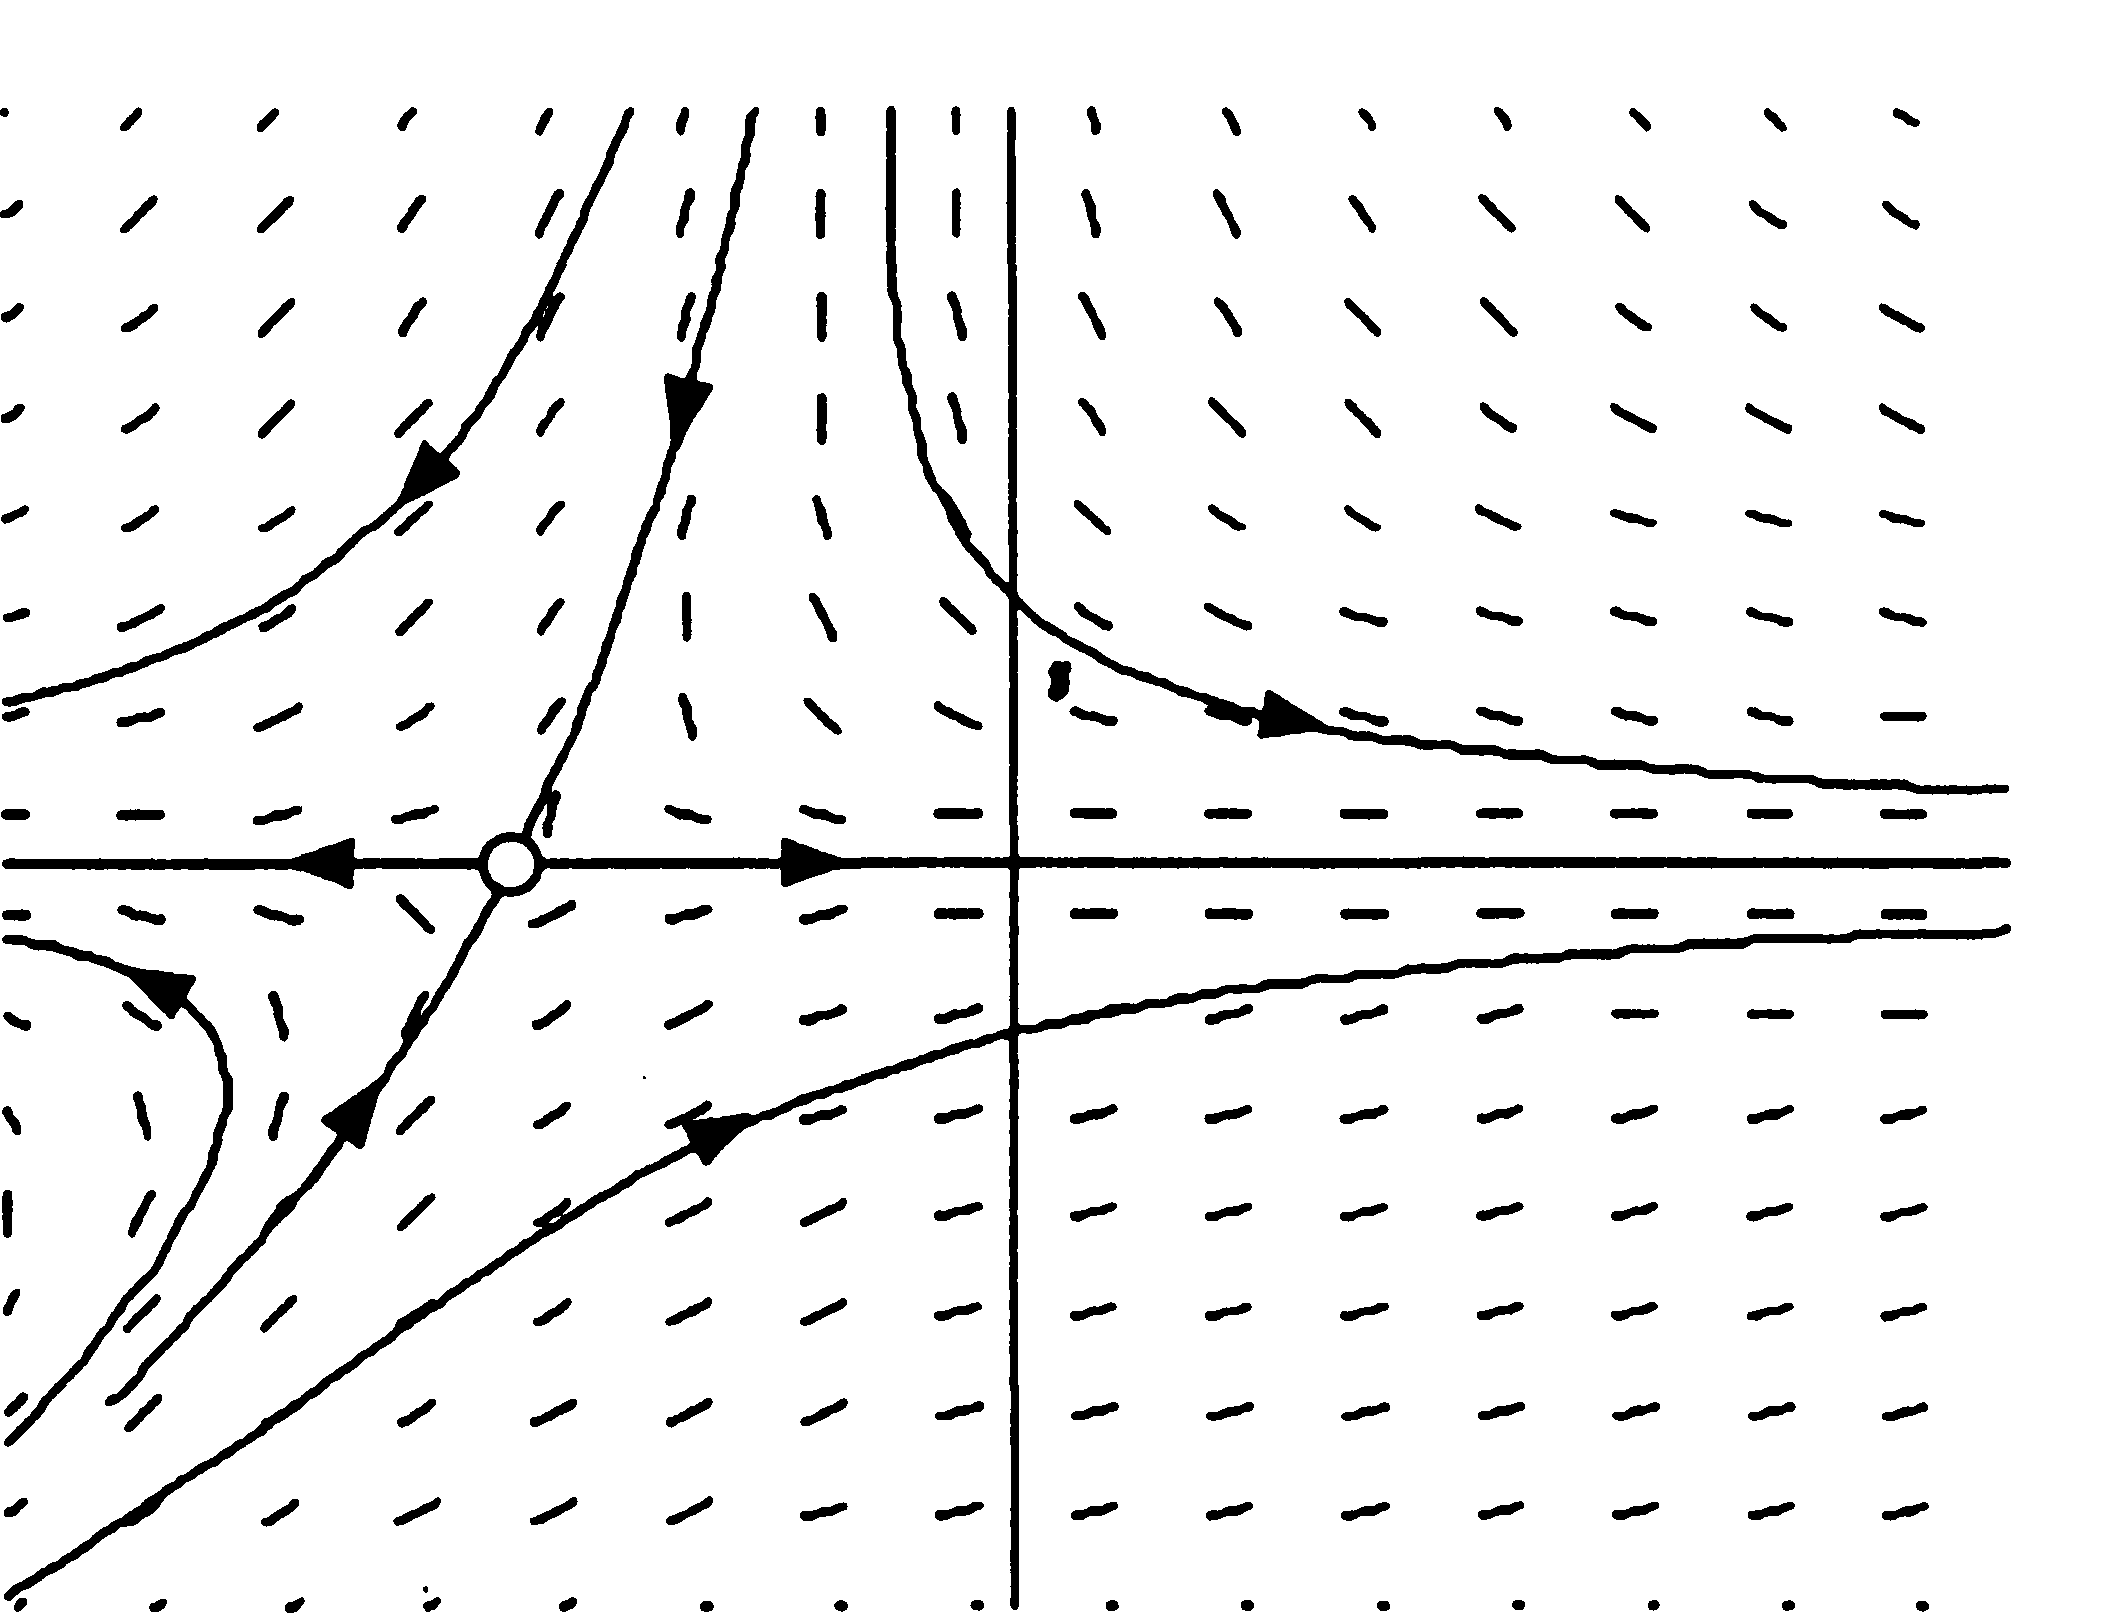
\includegraphics[width=0.82\textwidth]{images/Figures/figur-004.png}
\caption{Örnek 6.1.1 için yön alanı ve seçilmiş yörüngeler.}
\label{fig:6-1-4}
\end{figure}
\end{justify}

\section{Varlık, Teklik ve Topolojik Sonuçlar}

\begin{justify}
Şimdiye kadar biraz iyimser davrandık; bu aşamada genel doğrusal olmayan sistem
\begin{equation}
\dot{\mathbf{x}}=\mathbf{f}(\mathbf{x})
\end{equation}
için çözümlerin var olduğuna dair henüz bir güvencemiz yoktur. Neyse ki Bölüm 2.5'te verilen varlık ve teklik teoremi iki boyutlu sistemlere genelleştirilebilir. Ek bir zorluk içermediği için sonuç $n$ boyutlu sistemler için ifade edilir.

\textbf{Varlık ve Teklik Teoremi.} Başlangıç değer problemini ele alalım:
\begin{equation}
\dot{\mathbf{x}}=\mathbf{f}(\mathbf{x}), \qquad \mathbf{x}(0)=\mathbf{x}_0.
\end{equation}
$\mathbf{f}$ sürekli olsun ve tüm kısmi türevleri
\begin{equation}
\frac{\partial f_i}{\partial x_j}, \qquad i,j=1,\ldots,n,
\end{equation}
$D\subset \mathbb{R}^n$ olan açık ve bağlantılı bir kümede sürekli olsun. O hâlde $\mathbf{x}_0\in D$ için başlangıç değer probleminin $t=0$ etrafındaki bir $(-\tau,\tau)$ zaman aralığında bir çözümü vardır ve bu çözüm tektir.

Başka bir deyişle, $\mathbf{f}$ sürekli türevlenebilirse çözümlerin varlığı ve tekliği güvence altındadır. Teoremin ispatı $n=1$ durumu için yapılan ispata benzerdir ve diferansiyel denklemler üzerine yazılmış çoğu kaynakta bulunabilir. Teoremin daha güçlü biçimleri de vardır; ancak bu biçim çoğu uygulama için yeterlidir.

Bundan sonra, ele alınan tüm vektör alanlarının faz uzayındaki herhangi bir noktadan başlayan çözümlerin varlığını ve tekliğini sağlayacak kadar düzgün olduğunu kabul edeceğiz.

Varlık ve teklik teoreminin önemli bir sonucu vardır: farklı yörüngeler asla kesişmez. Eğer iki yörünge kesişseydi, aynı noktadan, yani kesişim noktasından başlayan iki farklı çözüm olurdu. Bu durum teoremin teklik kısmıyla çelişirdi. Daha sezgisel bir ifadeyle, bir yörünge aynı anda iki farklı yönde hareket edemez.

Yörüngeler kesişemediği için faz portreleri her zaman düzenli bir görünüme sahiptir. Aksi hâlde, birbirini kesen eğrilerden oluşan karmaşık bir düğüme dönüşebilirlerdi (Şekil~\ref{fig:6-2-1}). Varlık ve teklik teoremi bunun olmasını engeller.

\begin{figure}[H]
\centering
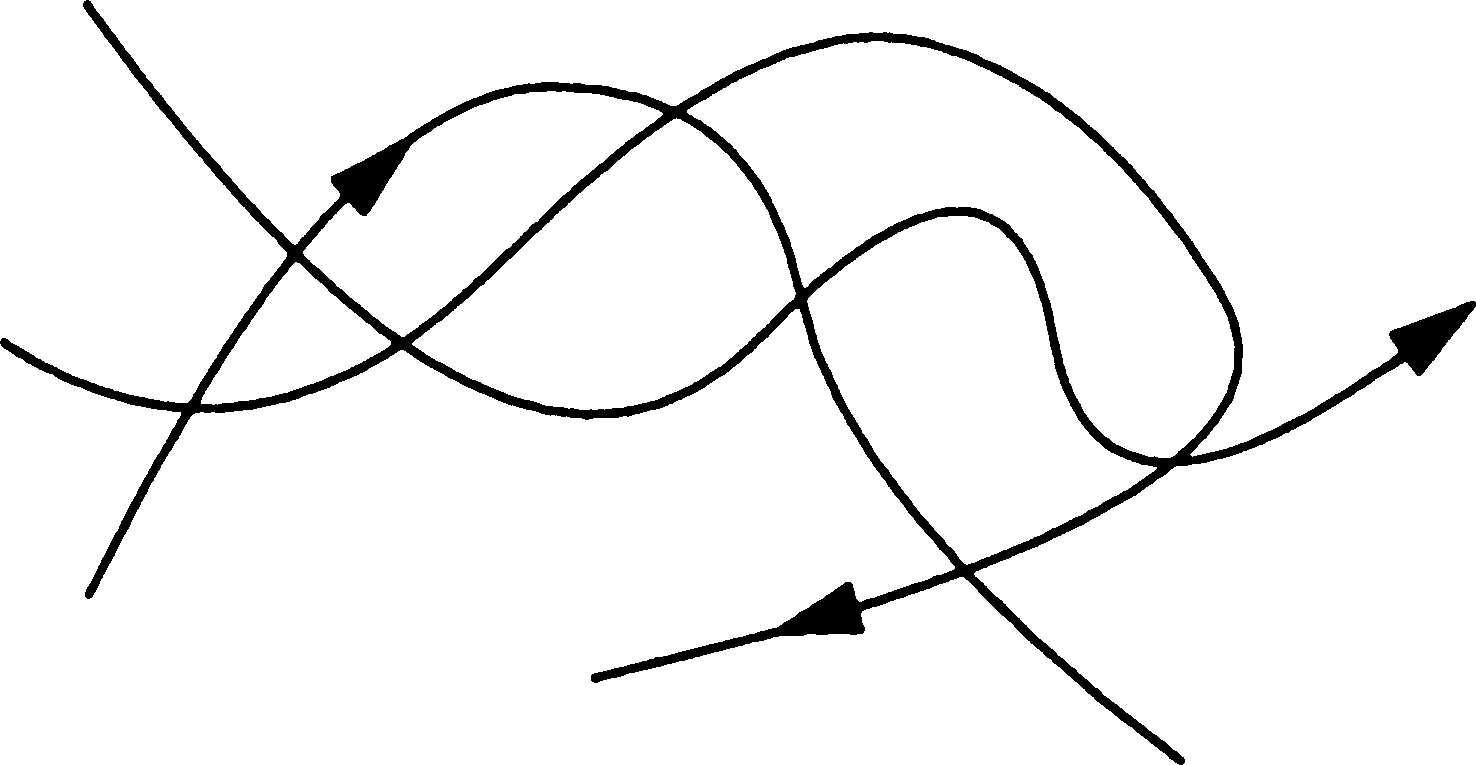
\includegraphics[width=0.82\textwidth]{images/Figures/figur-005.png}
\caption{Teklik özelliği olmasaydı ortaya çıkabilecek, birbirini kesen yörüngelerden oluşan düzensiz görünüm.}
\label{fig:6-2-1}
\end{figure}

İki boyutlu faz uzaylarında, daha yüksek boyutlu faz uzaylarından farklı olarak, bu sonuçların özellikle güçlü topolojik sonuçları vardır. Örneğin faz düzleminde kapalı bir $C$ yörüngesi bulunduğunu varsayalım. Bu durumda $C$ içinde başlayan herhangi bir yörünge sonsuza kadar bu bölgenin içinde hapsolur (Şekil~\ref{fig:6-2-2}).

\begin{figure}[H]
\centering
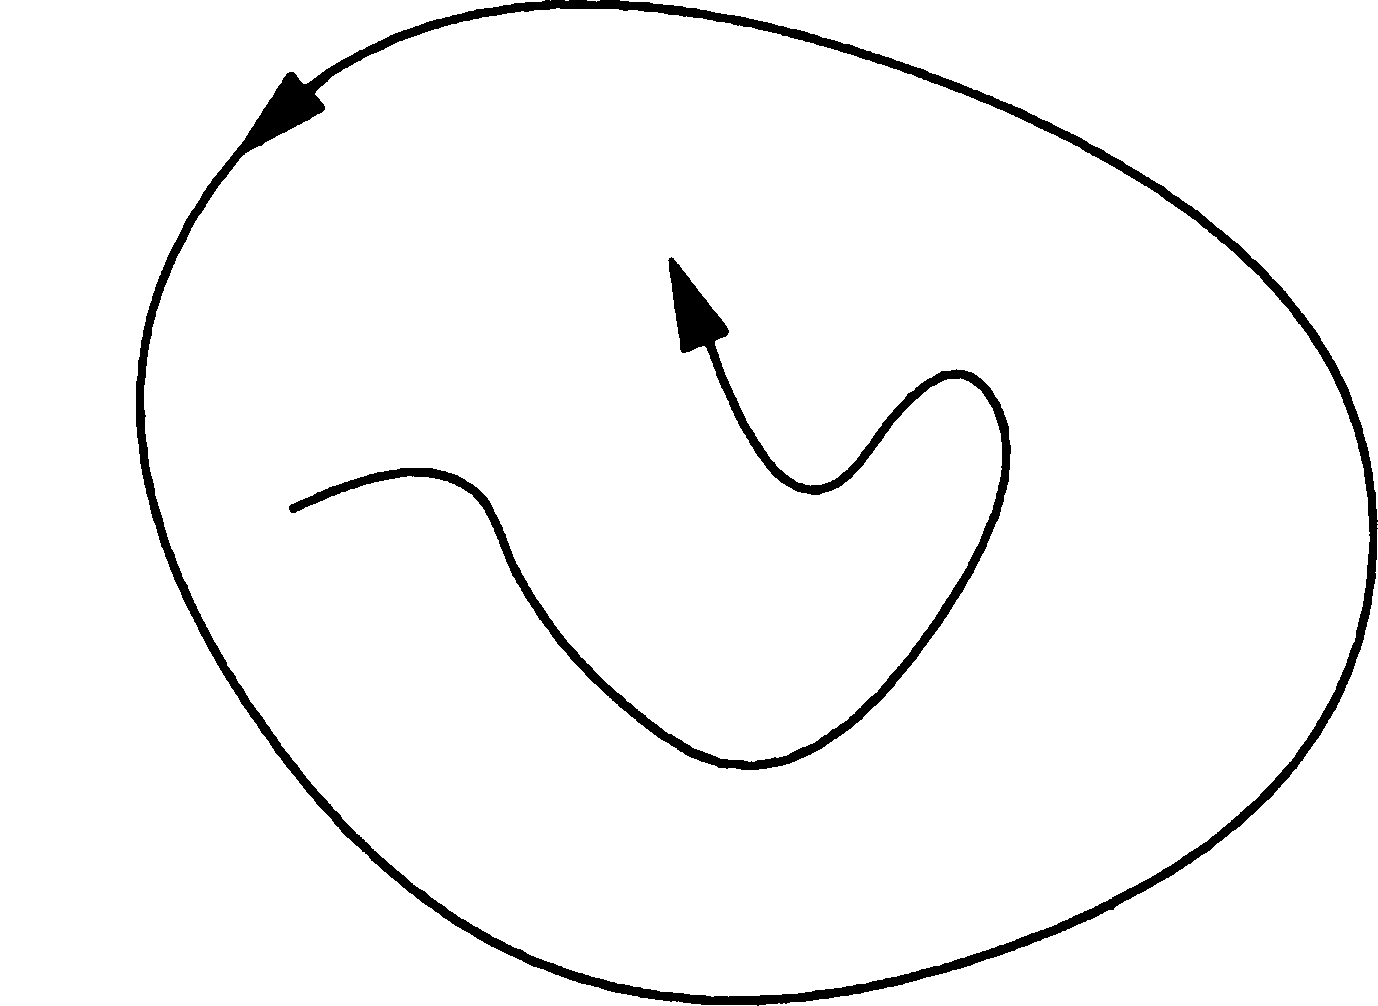
\includegraphics[width=0.82\textwidth]{images/Figures/figur-006.png}
\caption{Kapalı bir yörünge içinde başlayan yörüngenin içeride hapsolması.}
\label{fig:6-2-2}
\end{figure}

Peki böyle sınırlı bir yörüngenin sonu ne olur? Eğer $C$ içinde sabit noktalar varsa, yörünge elbette sonunda bunlardan birine yaklaşabilir. Fakat içeride hiç sabit nokta yoksa ne olur? Sezgileriniz yörüngenin sonsuza kadar gelişigüzel dolaşamayacağını söylüyorsa haklısınız. Düzlem üzerindeki vektör alanları için Poincaré--Bendixson teoremi şunu söyler: Bir yörünge kapalı ve sınırlı bir bölgede kalıyorsa ve bölgede sabit nokta yoksa, yörünge sonunda bir kapalı yörüngeye yaklaşmak zorundadır. Bu önemli teorem Bölüm 7.3'te tartışılacaktır.

Ancak hikâyenin bu kısmı daha sonra gelecektir. Önce sabit noktaları daha iyi tanımamız gerekir.
\end{justify}

\section{Sabit Noktalar ve Lineerleştirme}

\begin{justify}
Bu bölümde, daha önce tek boyutlu sistemler için geliştirilen lineerleştirme tekniğini genişletiyoruz. Umut edilen şey, bir sabit nokta yakınındaki faz portresinin, ona karşılık gelen doğrusal bir sistemin faz portresiyle yaklaşık olarak temsil edilebilmesidir.
\end{justify}

\subsection*{Lineerleştirilmiş Sistem}
\phantomsection
\addcontentsline{toc}{subsection}{Lineerleştirilmiş Sistem}

\begin{justify}
Aşağıdaki sistemi ele alalım:
\begin{align}
\dot{x} &= f(x,y),\\
\dot{y} &= g(x,y),
\end{align}
ve $(x^{*},y^{*})$ noktasının bir sabit nokta olduğunu varsayalım; yani
\begin{equation}
f(x^{*},y^{*})=0, \qquad g(x^{*},y^{*})=0.
\end{equation}
Sabit noktadan küçük bir sapmanın bileşenlerini
\begin{equation}
u=x-x^{*}, \qquad v=y-y^{*}
\end{equation}
ile gösterelim. Bu sapmanın büyüyüp büyümediğini ya da sönümlenip sönümlenmediğini görmek için $u$ ve $v$ için diferansiyel denklemler türetmemiz gerekir. Önce $u$ denklemini yazalım:
\begin{align}
\dot{u} &= \dot{x} && \text{çünkü } x^{*}\text{ sabittir},\\
&= f(x^{*}+u,y^{*}+v) && \text{yerine koyma ile},\\
&= f(x^{*},y^{*})+u\frac{\partial f}{\partial x}+v\frac{\partial f}{\partial y}+O(u^2,v^2,uv) && \text{Taylor açılımı ile},\\
&= u\frac{\partial f}{\partial x}+v\frac{\partial f}{\partial y}+O(u^2,v^2,uv) && \text{çünkü } f(x^{*},y^{*})=0.
\end{align}
Gösterimi sadeleştirmek için $\partial f/\partial x$ ve $\partial f/\partial y$ yazılmıştır; fakat bu kısmi türevlerin sabit nokta $(x^{*},y^{*})$ üzerinde değerlendirildiği unutulmamalıdır. Dolayısıyla bunlar fonksiyon değil, sayıdır. Ayrıca $O(u^2,v^2,uv)$ kısa gösterimi, $u$ ve $v$ cinsinden ikinci dereceden terimleri belirtir. $u$ ve $v$ küçük olduğundan, bu ikinci dereceden terimler son derece küçüktür.

Benzer şekilde
\begin{equation}
\dot{v}=u\frac{\partial g}{\partial x}+v\frac{\partial g}{\partial y}+O(u^2,v^2,uv)
\end{equation}
bulunur. Böylece $(u,v)$ sapması
\begin{equation}
\begin{pmatrix}\dot{u}\\ \dot{v}\end{pmatrix}
=
\begin{pmatrix}
\dfrac{\partial f}{\partial x} & \dfrac{\partial f}{\partial y}\\[0.3cm]
\dfrac{\partial g}{\partial x} & \dfrac{\partial g}{\partial y}
\end{pmatrix}
\begin{pmatrix}u\\ v\end{pmatrix}
+ \text{ikinci dereceden terimler}
\end{equation}
biçiminde evrilir. Buradaki
\begin{equation}
A=\begin{pmatrix}
\dfrac{\partial f}{\partial x} & \dfrac{\partial f}{\partial y}\\[0.3cm]
\dfrac{\partial g}{\partial x} & \dfrac{\partial g}{\partial y}
\end{pmatrix}_{(x^{*},y^{*})}
\end{equation}
matrisine sabit nokta $(x^{*},y^{*})$ üzerindeki Jacobian matrisi denir. Bu matris, Bölüm 2.4'te görülen $f'(x^{*})$ türevinin çok değişkenli karşılığıdır.

İkinci dereceden terimler çok küçük olduğundan, bunları tamamen ihmal etmek cazip görünür. Bunu yaptığımızda lineerleştirilmiş sistem elde edilir:
\begin{equation}
\begin{pmatrix}\dot{u}\\ \dot{v}\end{pmatrix}
=
\begin{pmatrix}
\dfrac{\partial f}{\partial x} & \dfrac{\partial f}{\partial y}\\[0.3cm]
\dfrac{\partial g}{\partial x} & \dfrac{\partial g}{\partial y}
\end{pmatrix}
\begin{pmatrix}u\\ v\end{pmatrix}.
\end{equation}
Bu sistemin dinamiği Bölüm 5.2'deki yöntemlerle analiz edilebilir.
\end{justify}

\subsection*{Küçük Doğrusal Olmayan Terimlerin Etkisi}
\phantomsection
\addcontentsline{toc}{subsection}{Küçük Doğrusal Olmayan Terimlerin Etkisi}

\begin{justify}
Denklemdeki ikinci dereceden terimleri ihmal etmek gerçekten güvenli midir? Başka bir deyişle, lineerleştirilmiş sistem $(x^{*},y^{*})$ yakınındaki faz portresinin nitel olarak doğru bir resmini verir mi? Yanıt, lineerleştirilmiş sistemin sabit noktası Bölüm 5.2'de tartışılan sınır durumlardan biri olmadığı sürece evettir. Yani lineerleştirilmiş sistem bir eyer, düğüm ya da spiral öngörüyorsa, özgün doğrusal olmayan sistemdeki sabit nokta da gerçekten eyer, düğüm ya da spiraldir. Bu sonucun ispatı için Andronov ve arkadaşlarına (1973) bakılabilir; somut bir örnek aşağıda verilmektedir.

Sınır durumlar, yani merkezler, yozlaşmış düğümler, yıldızlar ya da izole olmayan sabit noktalar çok daha hassastır. Bunlar küçük doğrusal olmayan terimler tarafından değiştirilebilir. Bunu Örnek 6.3.2'de ve Alıştırma 6.3.11'de göreceğiz.
\end{justify}

\subsection*{Örnek 6.3.1}
\phantomsection
\addcontentsline{toc}{subsection}{Örnek 6.3.1}

\begin{justify}
Aşağıdaki sistemin tüm sabit noktalarını bulun:
\begin{align}
\dot{x} &= -x+x^3,\\
\dot{y} &= -2y.
\end{align}
Ardından lineerleştirme kullanarak bu noktaları sınıflandırın. Son olarak, tam doğrusal olmayan sistem için faz portresini çıkararak sonuçlarınızı kontrol edin.

\textbf{Çözüm.} Sabit noktalar $\dot{x}=0$ ve $\dot{y}=0$ koşullarının aynı anda sağlandığı yerlerde ortaya çıkar. Bu nedenle $x=0$ ya da $x=\pm1$ ve $y=0$ olmalıdır. Böylece üç sabit nokta elde edilir:
\begin{equation}
(0,0), \qquad (1,0), \qquad (-1,0).
\end{equation}
Genel bir $(x,y)$ noktasındaki Jacobian matrisi
\begin{equation}
A=\begin{pmatrix}
\dfrac{\partial \dot{x}}{\partial x} & \dfrac{\partial \dot{x}}{\partial y}\\[0.3cm]
\dfrac{\partial \dot{y}}{\partial x} & \dfrac{\partial \dot{y}}{\partial y}
\end{pmatrix}
=
\begin{pmatrix}
-1+3x^2 & 0\\
0 & -2
\end{pmatrix}
\end{equation}
olur.

Şimdi $A$ matrisini sabit noktalarda değerlendirelim. $(0,0)$ noktasında
\begin{equation}
A=\begin{pmatrix}-1&0\\0&-2\end{pmatrix}
\end{equation}
bulunur; bu nedenle $(0,0)$ kararlı bir düğümdür. $(\pm1,0)$ noktalarında ise
\begin{equation}
A=\begin{pmatrix}2&0\\0&-2\end{pmatrix}
\end{equation}
olur; bu iki nokta da eyer noktasıdır.

Bu örnekte kararlı düğüm ve eyer noktaları sınır durumlar olmadığından, tam doğrusal olmayan sistemdeki sabit noktaların türlerinin doğru öngörüldüğünden emin olabiliriz.

Bu sonuç doğrusal olmayan sistem için doğrudan da kontrol edilebilir; çünkü $x$ ve $y$ denklemleri birbirinden ayrılmıştır. Sistem, birbirine dik iki bağımsız birinci mertebeden sistem gibi davranır. $y$ yönünde tüm yörüngeler üstel olarak $y=0$ doğrusuna yaklaşır. $x$ yönünde ise yörüngeler $x=0$ noktasına çekilir ve $x=\pm1$ noktalarından itilir. $x=0$ ve $x=\pm1$ düşey doğruları değişmezdir; çünkü bu doğrular üzerinde $\dot{x}=0$ olur. Dolayısıyla bu doğrular üzerinde başlayan bir yörünge sonsuza kadar bu doğrular üzerinde kalır. Benzer biçimde $y=0$ yatay doğrusu da değişmezdir. Denklemler $x\mapsto -x$ ve $y\mapsto -y$ dönüşümleri altında simetrik olduğundan faz portresi her iki eksene göre simetriktir. Bu bilgiler birleştirildiğinde Şekil~\ref{fig:6-3-1}'de gösterilecek faz portresine ulaşılır.

\begin{figure}[H]
\centering
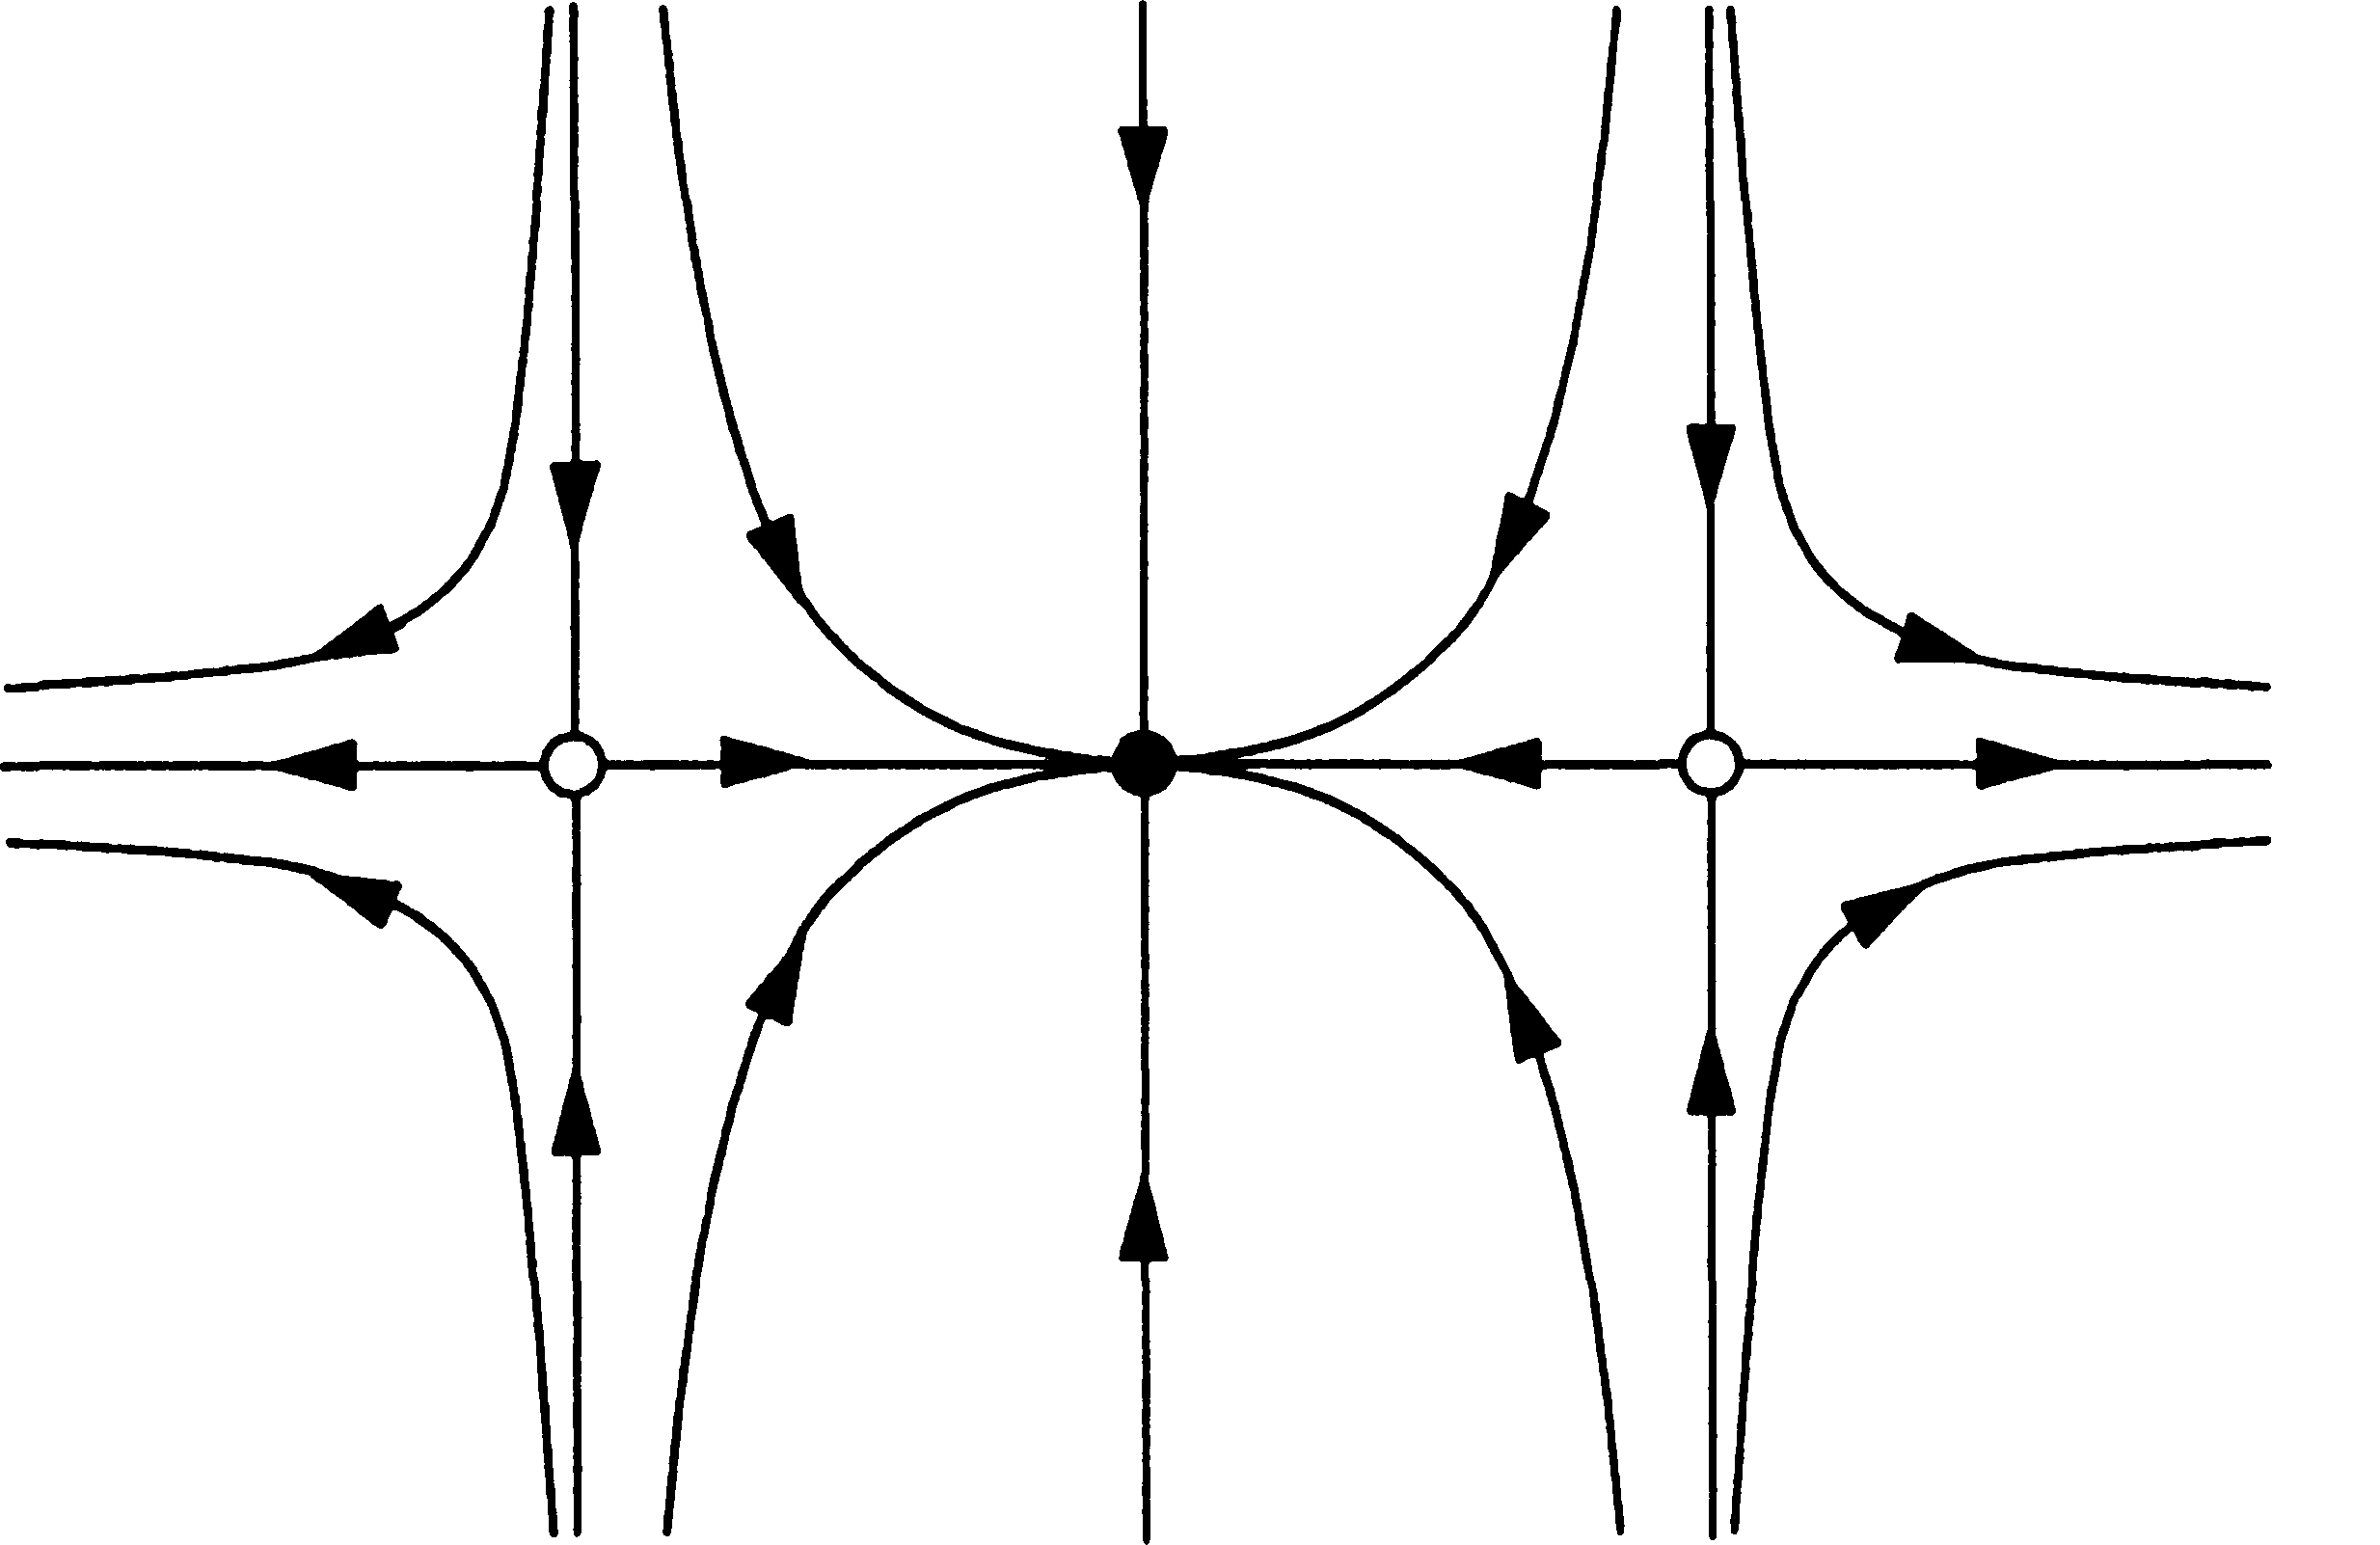
\includegraphics[width=0.82\textwidth]{images/Figures/figur-007.png}
\caption{Örnek 6.3.1 için doğrusal olmayan sistemin faz portresi.}
\label{fig:6-3-1}
\end{figure}

Bu resim, lineerleştirmeden beklendiği gibi $(0,0)$ noktasının kararlı düğüm, $(\pm1,0)$ noktalarının ise eyer olduğunu doğrular.
\end{justify}

\subsection*{Örnek 6.3.2}
\phantomsection
\addcontentsline{toc}{subsection}{Örnek 6.3.2}

\begin{justify}
Aşağıdaki sistemi ele alalım:
\begin{align}
\dot{x} &= -y+a x(x^2+y^2),\\
\dot{y} &= x+a y(x^2+y^2),
\end{align}
burada $a$ bir parametredir. Lineerleştirilmiş sistemin orijinin tüm $a$ değerleri için merkez olduğunu yanlış biçimde öngördüğünü; oysa gerçekte $a<0$ için orijinin kararlı spiral, $a>0$ için ise kararsız spiral olduğunu gösterin.

\textbf{Çözüm.} $(x^{*},y^{*})=(0,0)$ etrafındaki lineerleştirmeyi elde etmek için Jacobian matrisini doğrudan tanımdan hesaplayabiliriz. Ya da şu kısa yolu kullanabiliriz: Orijinde sabit noktası olan herhangi bir sistemde $x$ ve $y$, sabit noktadan sapmaları temsil eder; çünkü $u=x-x^{*}=x$ ve $v=y-y^{*}=y$ olur. Bu nedenle $x$ ve $y$ cinsinden doğrusal olmayan terimleri atarak lineerleştirme yapılabilir. Böylece lineerleştirilmiş sistem
\begin{align}
\dot{x} &= -y,\\
\dot{y} &= x
\end{align}
olur. Jacobian matrisi
\begin{equation}
A=\begin{pmatrix}0&-1\\1&0\end{pmatrix}
\end{equation}
şeklindedir. Bu matris için iz $\tau=0$ ve determinant $\Delta=1>0$ olduğundan lineerleştirmeye göre orijin her zaman bir merkezdir.

Doğrusal olmayan sistemi analiz etmek için kutupsal koordinatlara geçelim. $x=r\cos\theta$ ve $y=r\sin\theta$ olsun. $r$ için bir diferansiyel denklem türetmek amacıyla $x^2+y^2=r^2$ olduğuna dikkat edelim. Buradan
\begin{equation}
x\dot{x}+y\dot{y}=r\dot{r}
\end{equation}
elde edilir. $\dot{x}$ ve $\dot{y}$ yerine yazılırsa
\begin{align}
r\dot{r} &= x[-y+a x(x^2+y^2)]+y[x+a y(x^2+y^2)]\\
&= a(x^2+y^2)^2\\
&= ar^4
\end{align}
bulunur. Dolayısıyla
\begin{equation}
\dot{r}=ar^3.
\end{equation}
Alıştırma 6.3.12'de, $\theta$ için aşağıdaki diferansiyel denklemi türetmeniz istenir:
\begin{equation}
\dot{\theta}=\frac{x\dot{y}-y\dot{x}}{r^2}.
\end{equation}
$\dot{x}$ ve $\dot{y}$ yerine yazıldığında $\dot{\theta}=1$ bulunur. Böylece özgün sistem kutupsal koordinatlarda
\begin{align}
\dot{r} &= ar^3,\\
\dot{\theta} &= 1
\end{align}
biçimine dönüşür.

Bu biçimde sistemi analiz etmek kolaydır; çünkü radyal ve açısal hareketler birbirinden bağımsızdır. Tüm yörüngeler orijin etrafında sabit açısal hız $\dot{\theta}=1$ ile döner.

Radyal hareket $a$ değerine bağlıdır ve Şekil~\ref{fig:6-3-2}'de gösterilecektir. Eğer $a<0$ ise $t\to\infty$ iken $r(t)$ monoton olarak $0$'a gider. Bu durumda orijin kararlı spiraldir. Ancak sönüm çok yavaştır; bu durum bilgisayar tarafından üretilen yörüngelerde de görülebilir. Eğer $a=0$ ise tüm $t$ değerleri için $r(t)=r_0$ olur ve orijin merkezdir. Son olarak $a>0$ ise $r(t)$ monoton olarak sonsuza gider ve orijin kararsız spiraldir.

\begin{figure}[H]
\centering
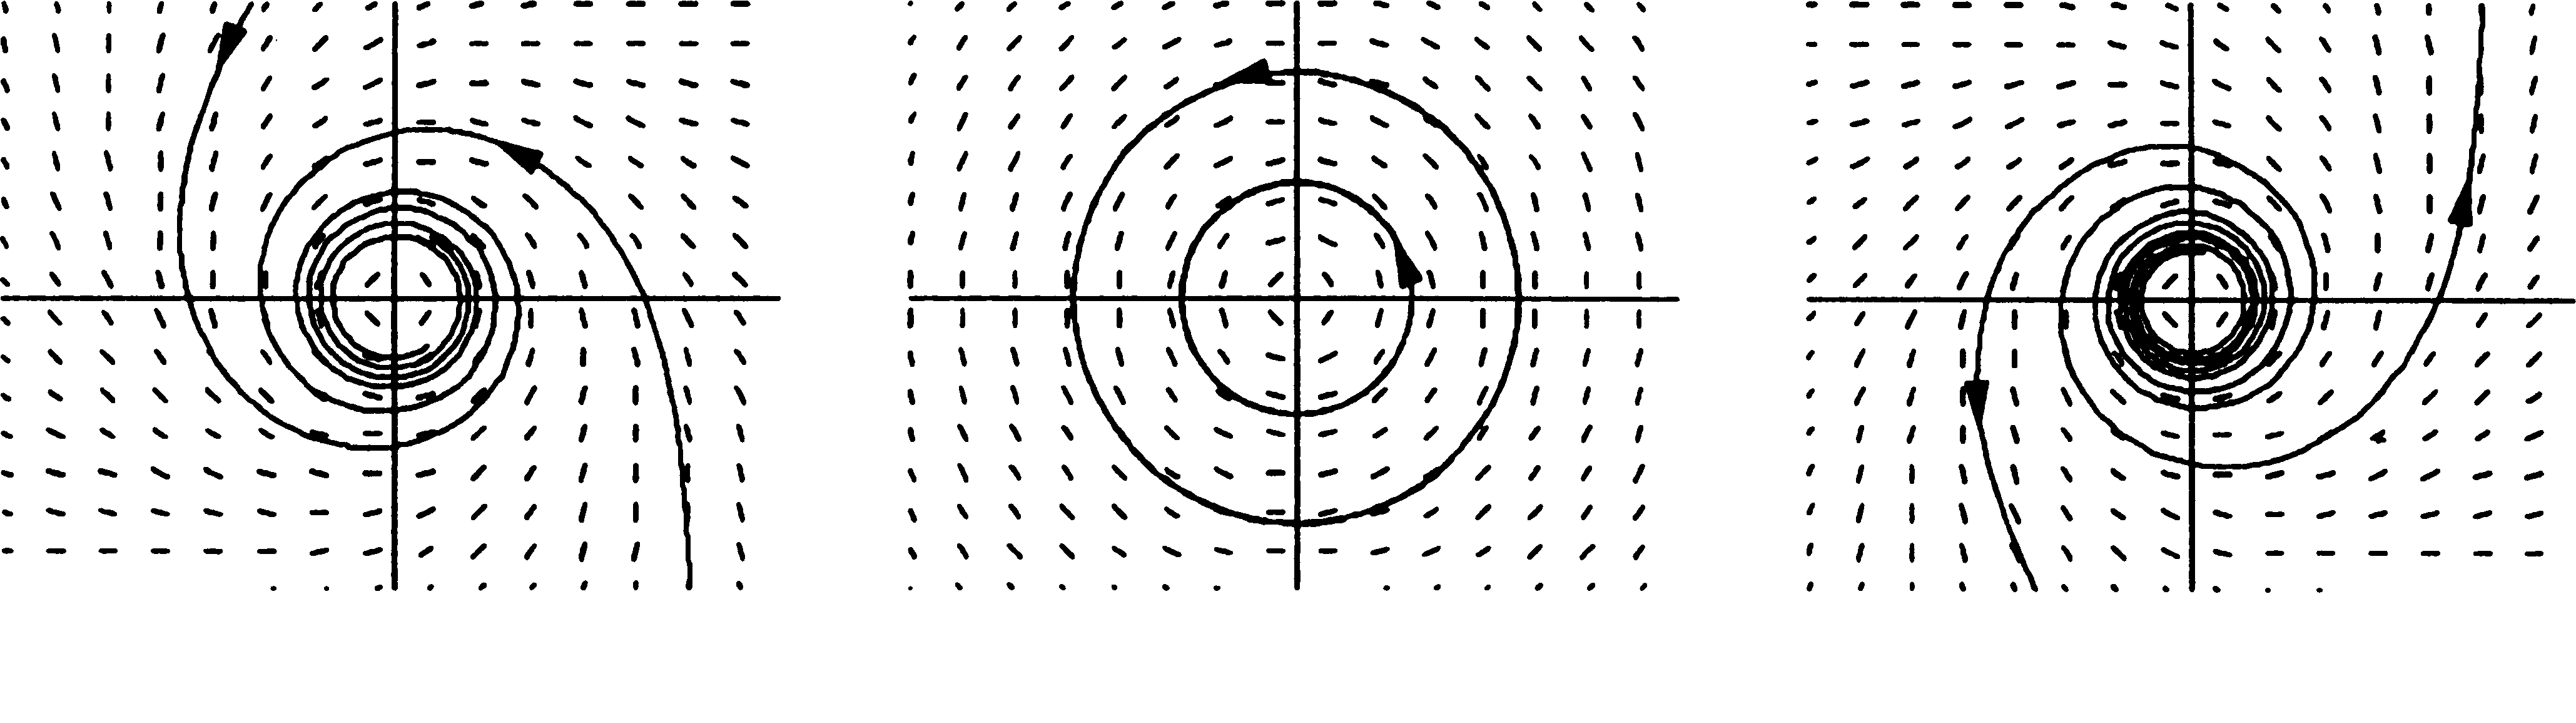
\includegraphics[width=0.82\textwidth]{images/Figures/figur-008.png}
\caption{Parametre değerlerine göre orijin yakınındaki davranış: $a<0$, $a=0$ ve $a>0$.}
\label{fig:6-3-2}
\end{figure}

Artık merkezlerin neden bu kadar hassas olduğunu görebiliriz: Tüm yörüngelerin bir çevrimden sonra kusursuz biçimde kapanması gerekir. En küçük bir sapma merkezi spirale dönüştürür.
\end{justify}

\subsection*{Hiperbolik Sabit Noktalar, Topolojik Eşdeğerlik ve Yapısal Kararlılık}
\phantomsection
\addcontentsline{toc}{subsection}{Hiperbolik Sabit Noktalar, Topolojik Eşdeğerlik ve Yapısal Kararlılık}

\begin{justify}
Benzer biçimde, yıldızlar ve yozlaşmış düğümler de küçük doğrusal olmayan etkilerle değiştirilebilir; fakat merkezlerden farklı olarak bunların kararlılığı değişmez. Örneğin kararlı bir yıldız, kararlı bir spirale dönüşebilir; fakat kararsız bir spirale dönüşmez. Bu durum, doğrusal sistemlerin sınıflandırılması düşünüldüğünde makuldür: yıldızlar ve yozlaşmış düğümler kararlı ya da kararsız bölgenin içinde yer alırken, merkezler kararlılık ile kararsızlık arasındaki hassas sınırda bulunur.

Eğer yörüngelerin ayrıntılı geometrisiyle değil yalnızca kararlılıkla ilgileniyorsak, sabit noktaları daha kaba biçimde şöyle sınıflandırabiliriz:

\textbf{Sağlam durumlar:}
\begin{itemize}
\item \textbf{İticiler} ya da \textbf{kaynaklar}: Her iki özdeğerin reel kısmı pozitiftir.
\item \textbf{Çekiciler} ya da \textbf{yutaklar}: Her iki özdeğerin reel kısmı negatiftir.
\item \textbf{Eyerler}: Özdeğerlerden biri pozitif, diğeri negatiftir.
\end{itemize}

\textbf{Marjinal durumlar:}
\begin{itemize}
\item \textbf{Merkezler}: Her iki özdeğer saf sanaldır.
\item \textbf{Daha yüksek mertebeden ve izole olmayan sabit noktalar}: En az bir özdeğer sıfırdır.
\end{itemize}

Dolayısıyla kararlılık açısından marjinal durumlar, en az bir özdeğerin $\operatorname{Re}(\lambda)=0$ koşulunu sağladığı durumlardır.

Her iki özdeğer için $\operatorname{Re}(\lambda)\neq0$ ise sabit nokta genellikle \textbf{hiperbolik} olarak adlandırılır. Bu ad biraz talihsizdir; çünkü kulağa yalnızca eyer noktası anlamına geliyormuş gibi gelir, ancak standart terim hâline gelmiştir. Hiperbolik sabit noktalar dayanıklıdır; kararlılık türleri küçük doğrusal olmayan terimlerden etkilenmez. Hiperbolik olmayan sabit noktalar ise hassas olanlardır.

Doğru üzerindeki vektör alanları bağlamında hiperbolikliğin basit bir örneğini daha önce gördük. Bölüm 2.4'te, $f'(x^{*})\neq0$ olduğu sürece sabit noktanın kararlılığının lineerleştirme tarafından doğru biçimde öngörüldüğünü gördük. Bu koşul, $\operatorname{Re}(\lambda)\neq0$ koşulunun tam karşılığıdır.

Bu fikirler daha yüksek mertebeden sistemlere de düzgün biçimde genellenir. $n$ mertebeli bir sistemin sabit noktası, lineerleştirmenin tüm özdeğerleri sanal eksen dışında yer alıyorsa hiperboliktir; yani $i=1,\ldots,n$ için $\operatorname{Re}(\lambda_i)\neq0$ olmalıdır. Önemli Hartman--Grobman teoremi, hiperbolik bir sabit nokta yakınındaki yerel faz portresinin lineerleştirmenin faz portresiyle \textit{topolojik olarak eşdeğer} olduğunu söyler. Özellikle, sabit noktanın kararlılık türü lineerleştirme tarafından doğru biçimde yakalanır.

Burada topolojik eşdeğerlik, bir yerel faz portresini diğerine taşıyan bir homeomorfizmanın, yani sürekli tersi olan sürekli bir deformasyonun bulunması anlamına gelir. Bu dönüşüm yörüngeleri yörüngelere götürür ve zaman yönünü, yani okların yönünü korur.

Sezgisel olarak iki faz portresi, biri diğerinin bozulmuş bir biçimiyse topolojik olarak eşdeğerdir. Eğme ve bükmeye izin vardır; fakat yırtmaya izin yoktur. Dolayısıyla kapalı yörüngeler kapalı kalmalı, eyer noktalarını birleştiren yörüngeler kopmamalıdır.

Hiperbolik sabit noktalar ayrıca yapısal kararlılık denen önemli genel kavramı da gösterir. Bir faz portresi, vektör alanına yapılan keyfî derecede küçük bir bozunumla topolojisi değiştirilemiyorsa yapısal olarak kararlıdır. Örneğin bir eyer noktasının faz portresi yapısal olarak kararlıdır; ancak bir merkezin faz portresi değildir. Çünkü keyfî derecede küçük bir sönüm, merkezi spirale dönüştürür.
\end{justify}


\newpage

\section{Tavşanlara Karşı Koyunlar}

\begin{justify}
Bu bölümde faz düzlemi analizinin klasik bir örneği olarak iki tür arasındaki rekabet modeli ele alınır. Türler tavşanlar ve koyunlar olarak düşünülür. Her iki türün de aynı sınırlı besin kaynağı için rekabet ettiği varsayılır.

Bu varsayımları içeren Lotka--Volterra tipi model
\begin{align}
\dot{x} &= x(3-x-2y),\\
\dot{y} &= y(2-y-x)
\end{align}
şeklindedir. Burada
\begin{equation}
x(t)=\text{tavşan popülasyonu}, \qquad y(t)=\text{koyun popülasyonu}
\end{equation}
olup $x,y\ge 0$ kabul edilir.

Sabit noktalar $\dot{x}=0$ ve $\dot{y}=0$ denklemlerinin birlikte çözülmesiyle bulunur:
\begin{equation}
(0,0), \qquad (0,2), \qquad (3,0), \qquad (1,1).
\end{equation}
Sınıflandırma için Jacobian matrisi
\begin{equation}
A=\begin{pmatrix}
\dfrac{\partial \dot{x}}{\partial x} & \dfrac{\partial \dot{x}}{\partial y}\\[0.3cm]
\dfrac{\partial \dot{y}}{\partial x} & \dfrac{\partial \dot{y}}{\partial y}
\end{pmatrix}
=
\begin{pmatrix}
3-2x-2y & -2x\\
-y & 2-x-2y
\end{pmatrix}
\end{equation}
olur.

$(0,0)$ noktasında $A=\begin{pmatrix}3&0\\0&2\end{pmatrix}$ olduğundan bu nokta kararsız düğümdür (Şekil~\ref{fig:6-4-1}).
\begin{figure}[H]
\centering
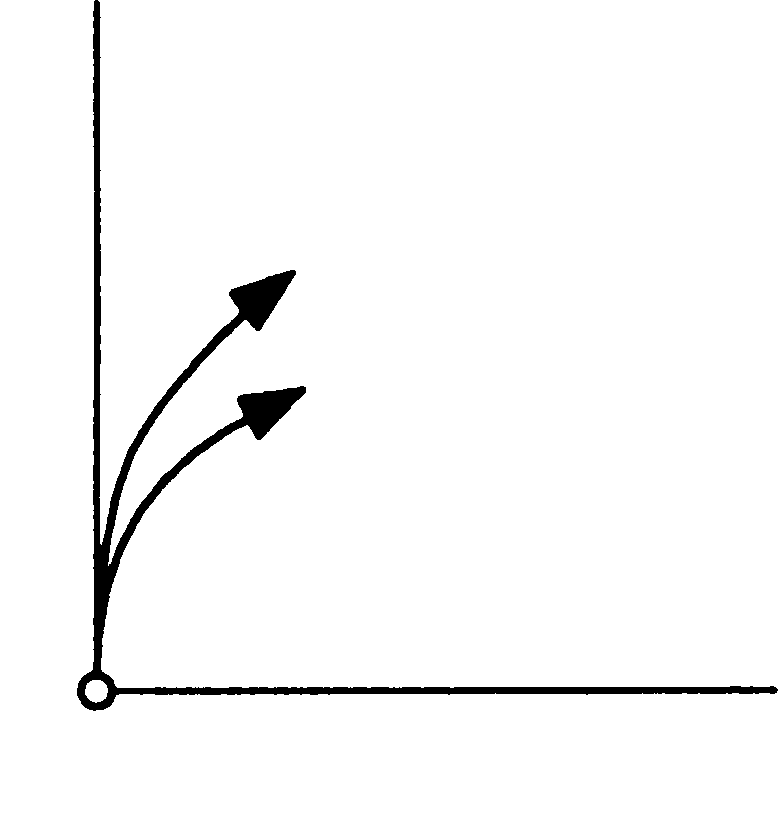
\includegraphics[width=0.82\textwidth]{images/Figures/figur-009.png}
\caption{Tavşan--koyun modelinde $(0,0)$ yakınındaki kararsız düğüm.}
\label{fig:6-4-1}
\end{figure}

$(0,2)$ noktasında $A=\begin{pmatrix}-1&0\\-2&-2\end{pmatrix}$ olduğundan bu nokta kararlı düğümdür (Şekil~\ref{fig:6-4-2}).
\begin{figure}[H]
\centering
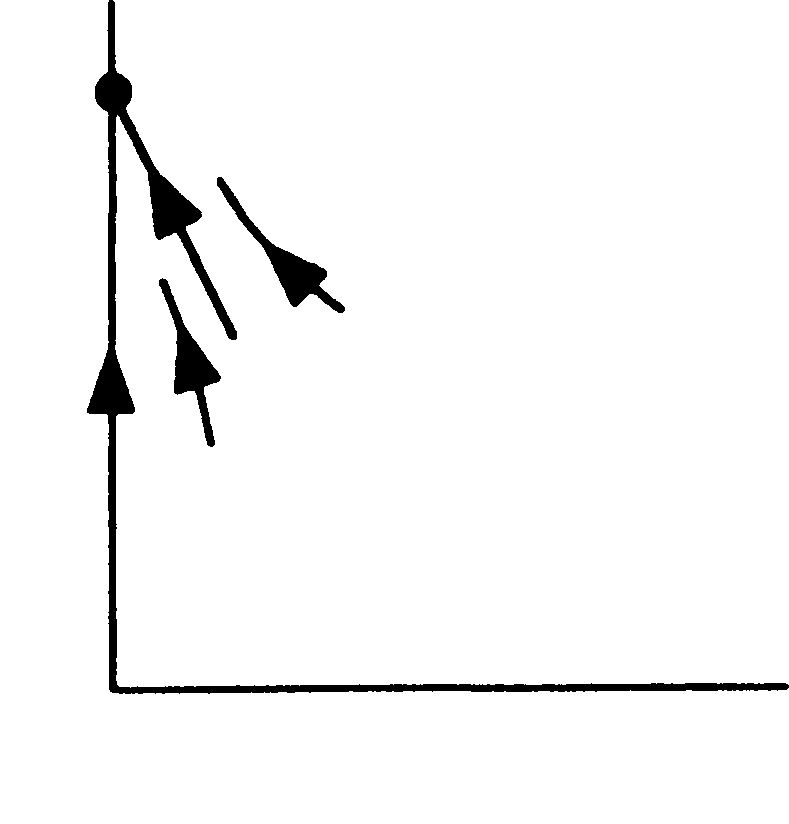
\includegraphics[width=0.82\textwidth]{images/Figures/figur-010.png}
\caption{Tavşan--koyun modelinde $(0,2)$ yakınındaki kararlı düğüm.}
\label{fig:6-4-2}
\end{figure}

$(3,0)$ noktasında
\begin{equation}
A=\begin{pmatrix}-3&-6\\0&-1\end{pmatrix}, \qquad \lambda=-3,-1
\end{equation}
olur. Bu nokta da kararlı düğümdür (Şekil~\ref{fig:6-4-3}).
\begin{figure}[H]
\centering
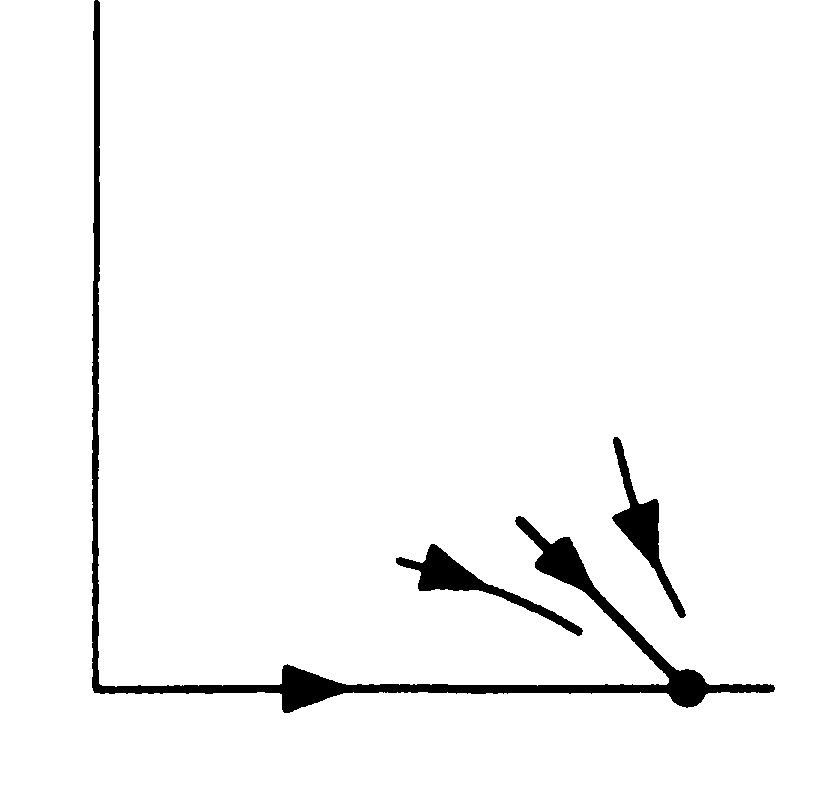
\includegraphics[width=0.82\textwidth]{images/Figures/figur-011.png}
\caption{Tavşan--koyun modelinde $(3,0)$ yakınındaki kararlı düğüm.}
\label{fig:6-4-3}
\end{figure}

$(1,1)$ noktasında
\begin{equation}
A=\begin{pmatrix}-1&-2\\-1&-1\end{pmatrix}, \qquad \lambda=-1\pm\sqrt{2}
\end{equation}
olduğundan bu nokta bir eyer noktasıdır (Şekil~\ref{fig:6-4-4}).
\begin{figure}[H]
\centering
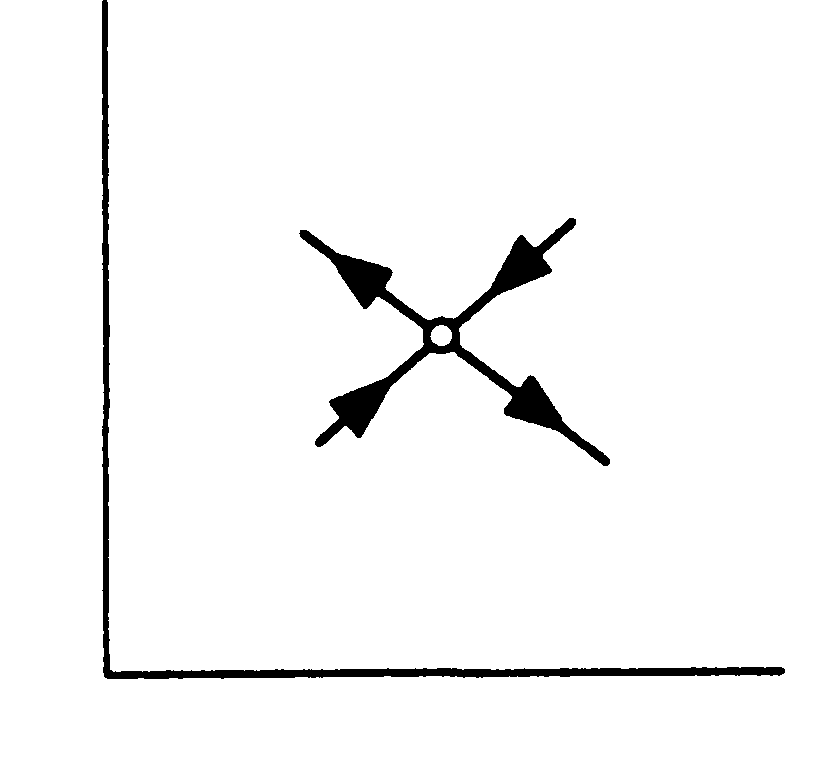
\includegraphics[width=0.82\textwidth]{images/Figures/figur-012.png}
\caption{Tavşan--koyun modelinde $(1,1)$ yakınındaki eyer noktası.}
\label{fig:6-4-4}
\end{figure}

Yerel faz portreleri birleştirildiğinde genel taslak elde edilir (Şekil~\ref{fig:6-4-5}). Eyer noktasına yaklaşan özel yörüngeler eyerin kararlı manifoldunu oluşturur (Şekil~\ref{fig:6-4-6}). Bilgisayar üretimli faz portresi Şekil~\ref{fig:6-4-7}'de gösterilecektir.
\begin{figure}[H]
\centering
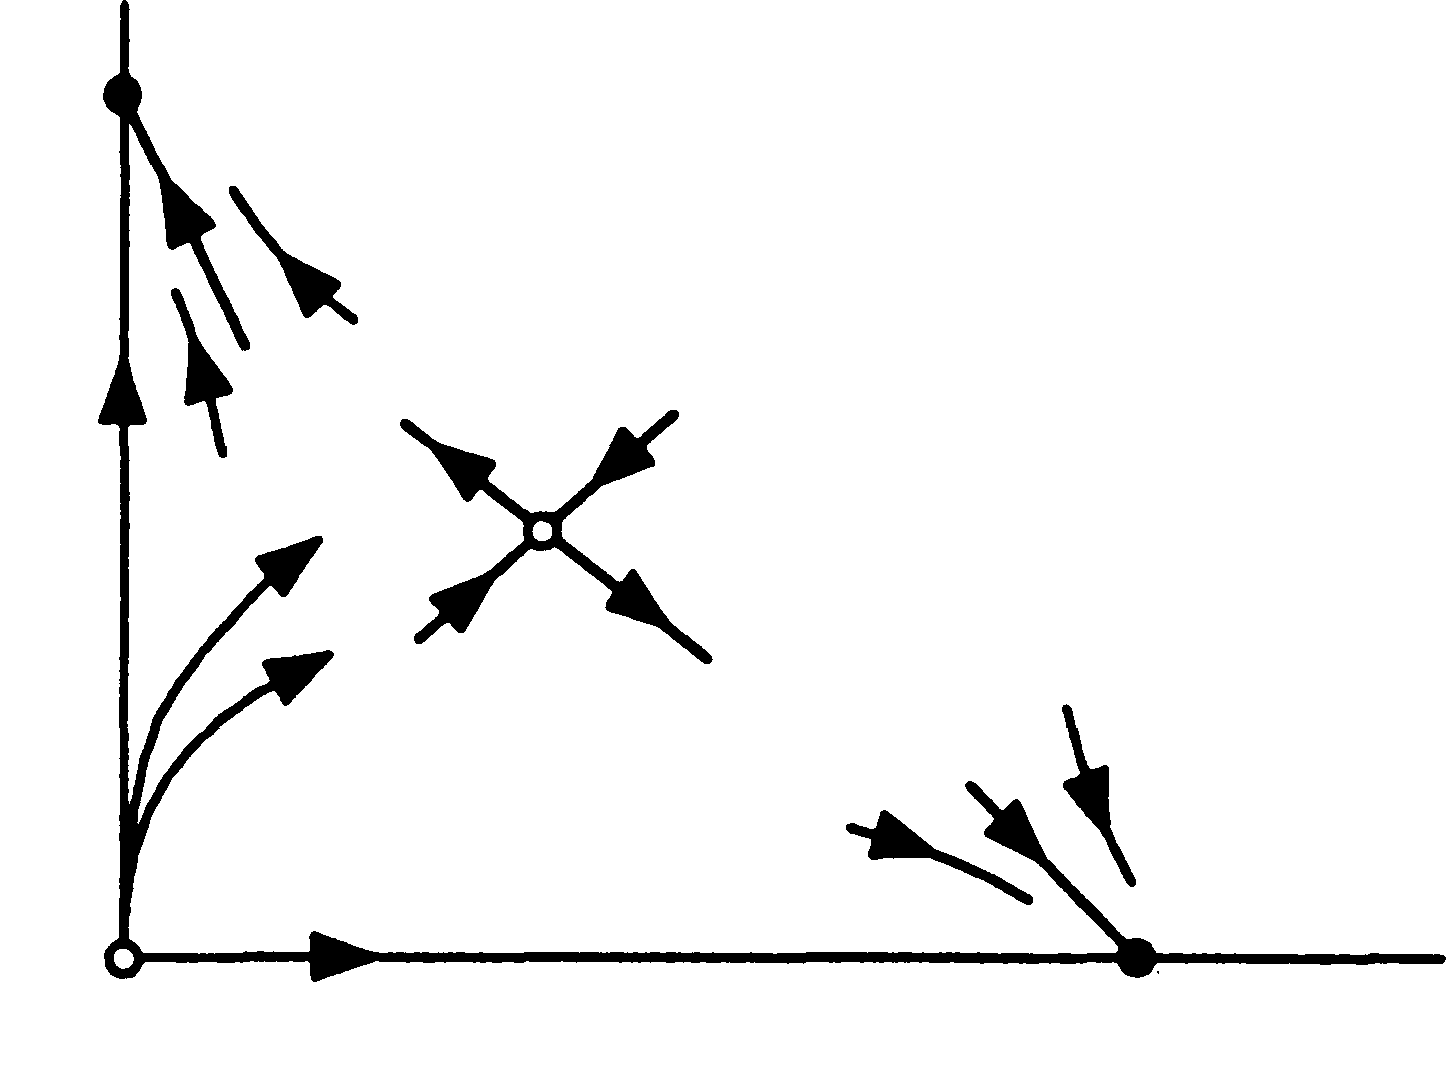
\includegraphics[width=0.82\textwidth]{images/Figures/figur-013.png}
\caption{Yerel faz portrelerinin birleştirilmesiyle elde edilen genel taslak.}
\label{fig:6-4-5}
\end{figure}
\begin{figure}[H]
\centering
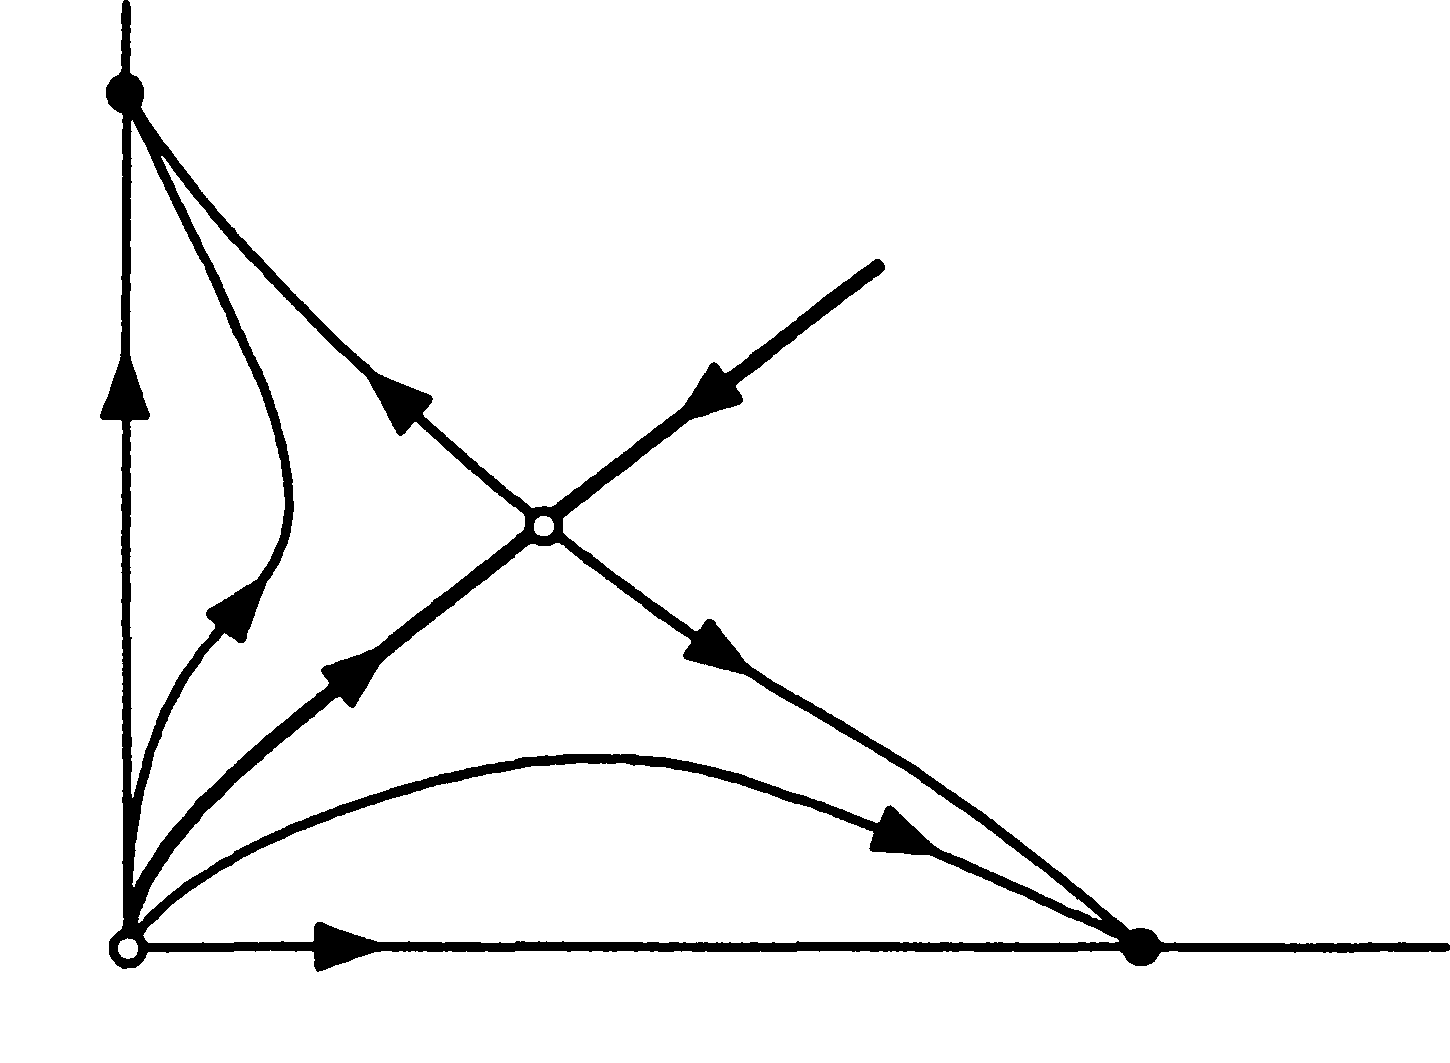
\includegraphics[width=0.82\textwidth]{images/Figures/figur-014.png}
\caption{Eyerin kararlı manifoldu ile tamamlanan faz portresi taslağı.}
\label{fig:6-4-6}
\end{figure}
\begin{figure}[H]
\centering
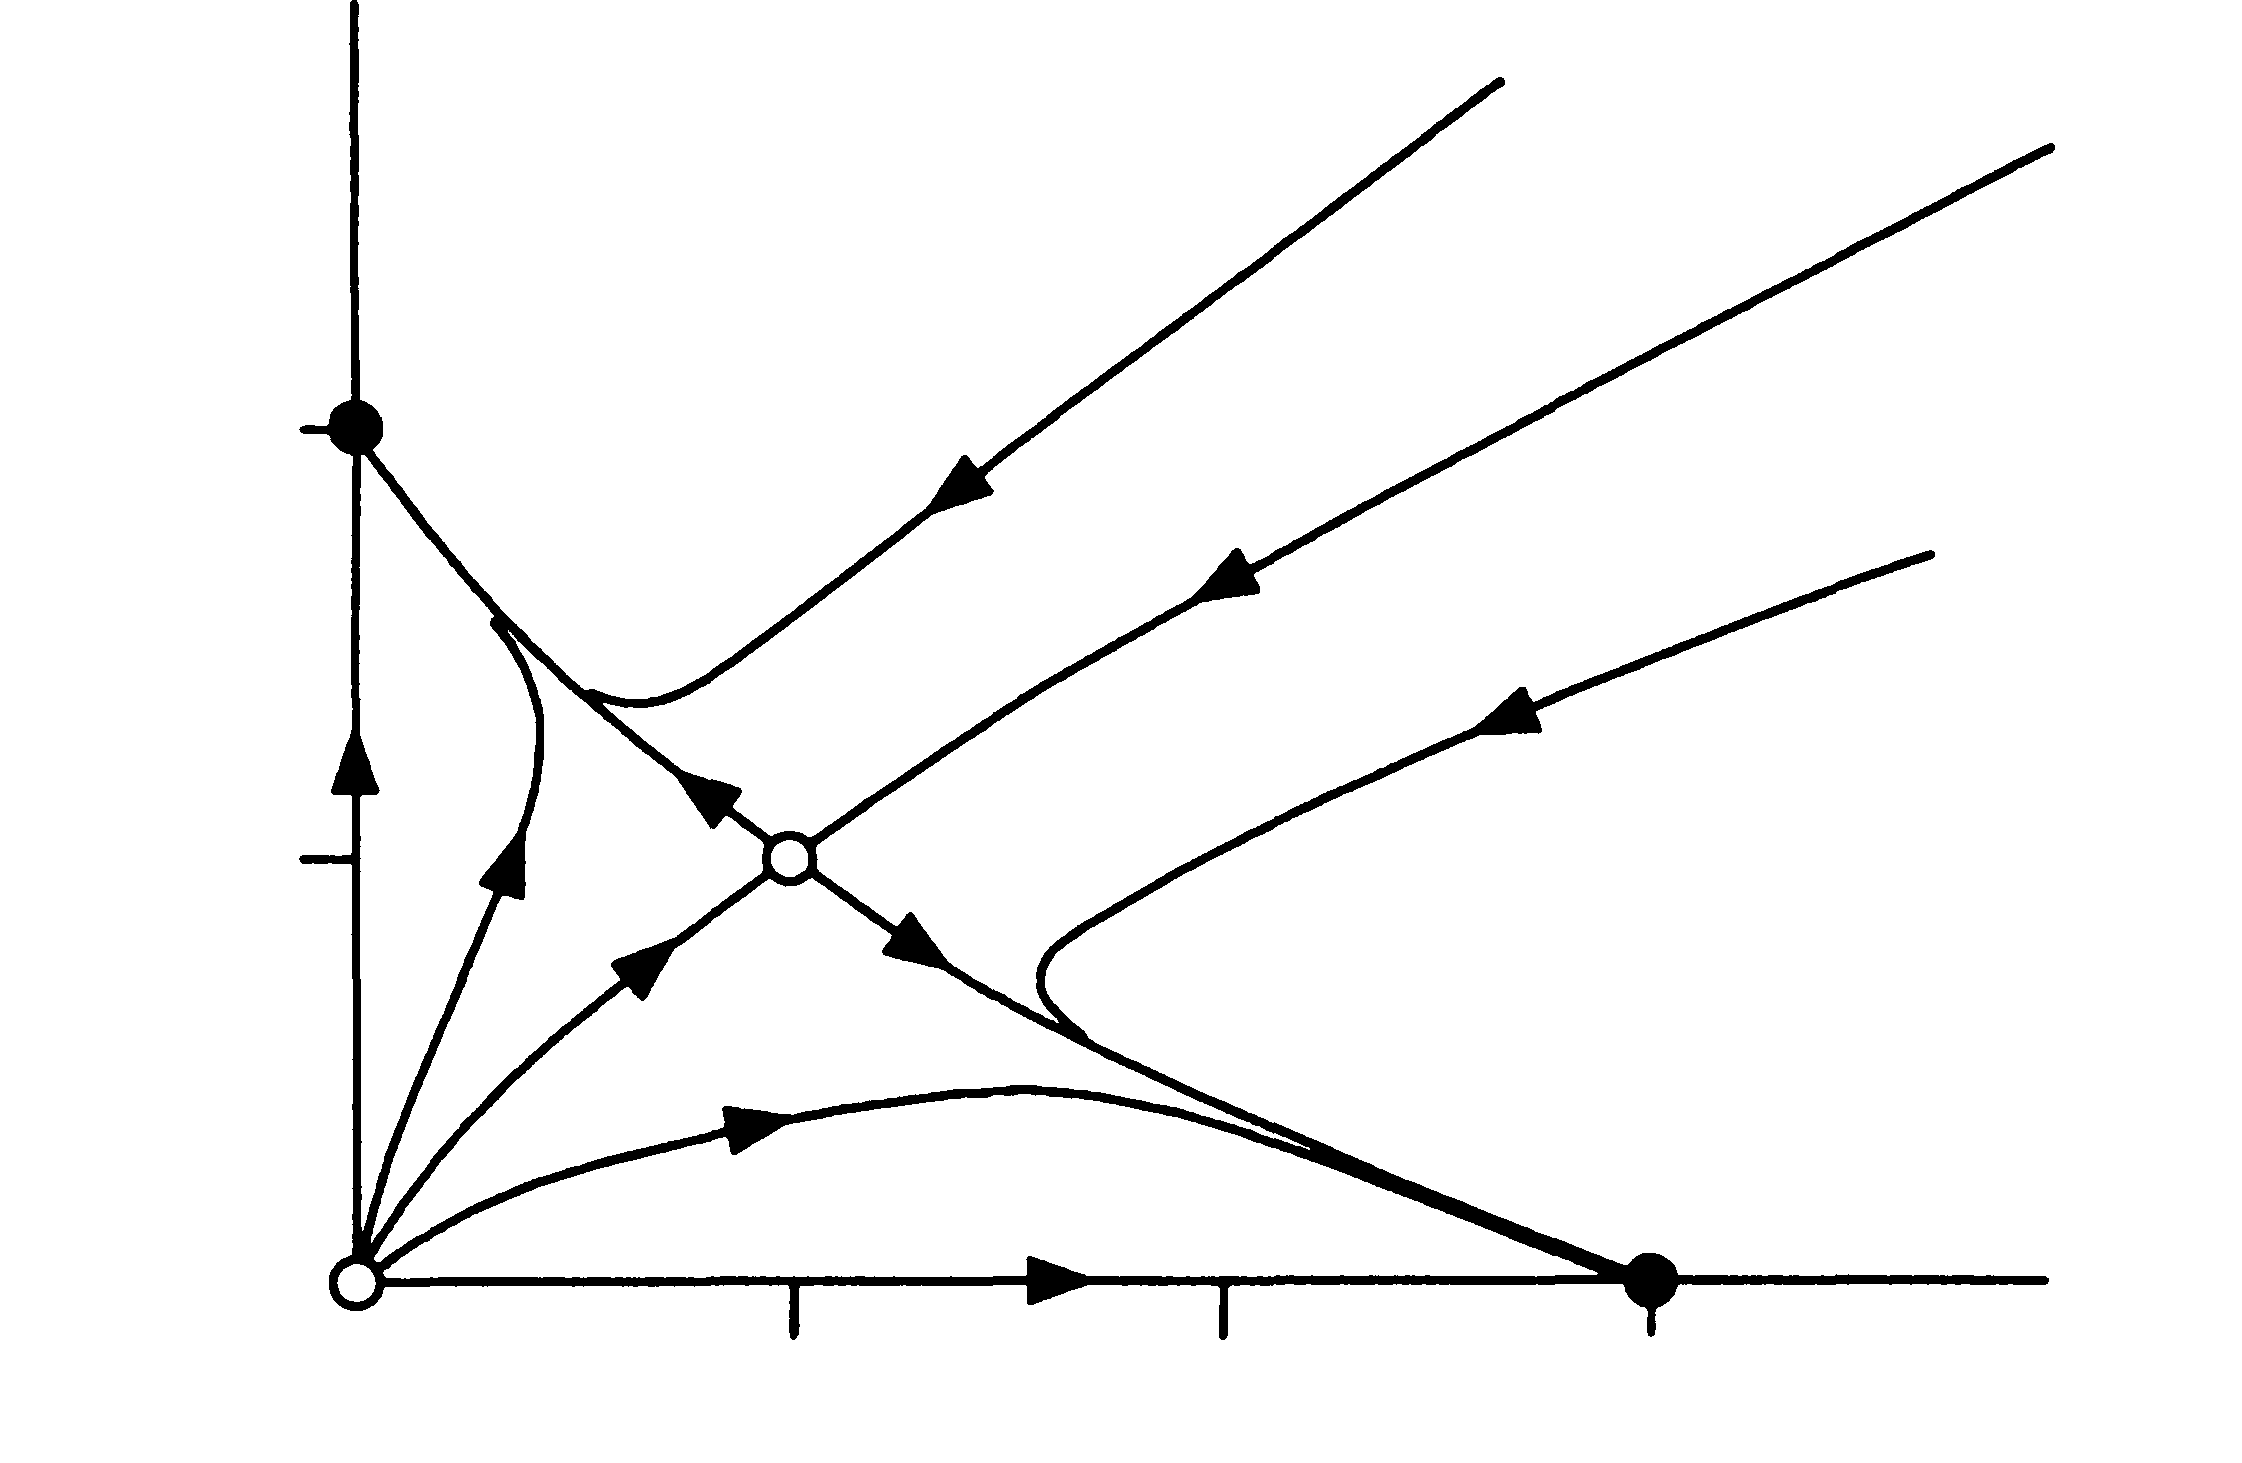
\includegraphics[width=0.82\textwidth]{images/Figures/figur-015.png}
\caption{Tavşan--koyun modeli için bilgisayar üretimli faz portresi.}
\label{fig:6-4-7}
\end{figure}

Biyolojik yorum şudur: Kararlı manifoldun altında başlayan yörüngeler koyunların, üstünde başlayan yörüngeler ise tavşanların yok oluşuna yol açar. Bu durum rekabetçi dışlama ilkesiyle ilişkilidir. $(3,0)$ düğümünün çekim havzası Şekil~\ref{fig:6-4-8}'de gösterilecektir.
\begin{figure}[H]
\centering
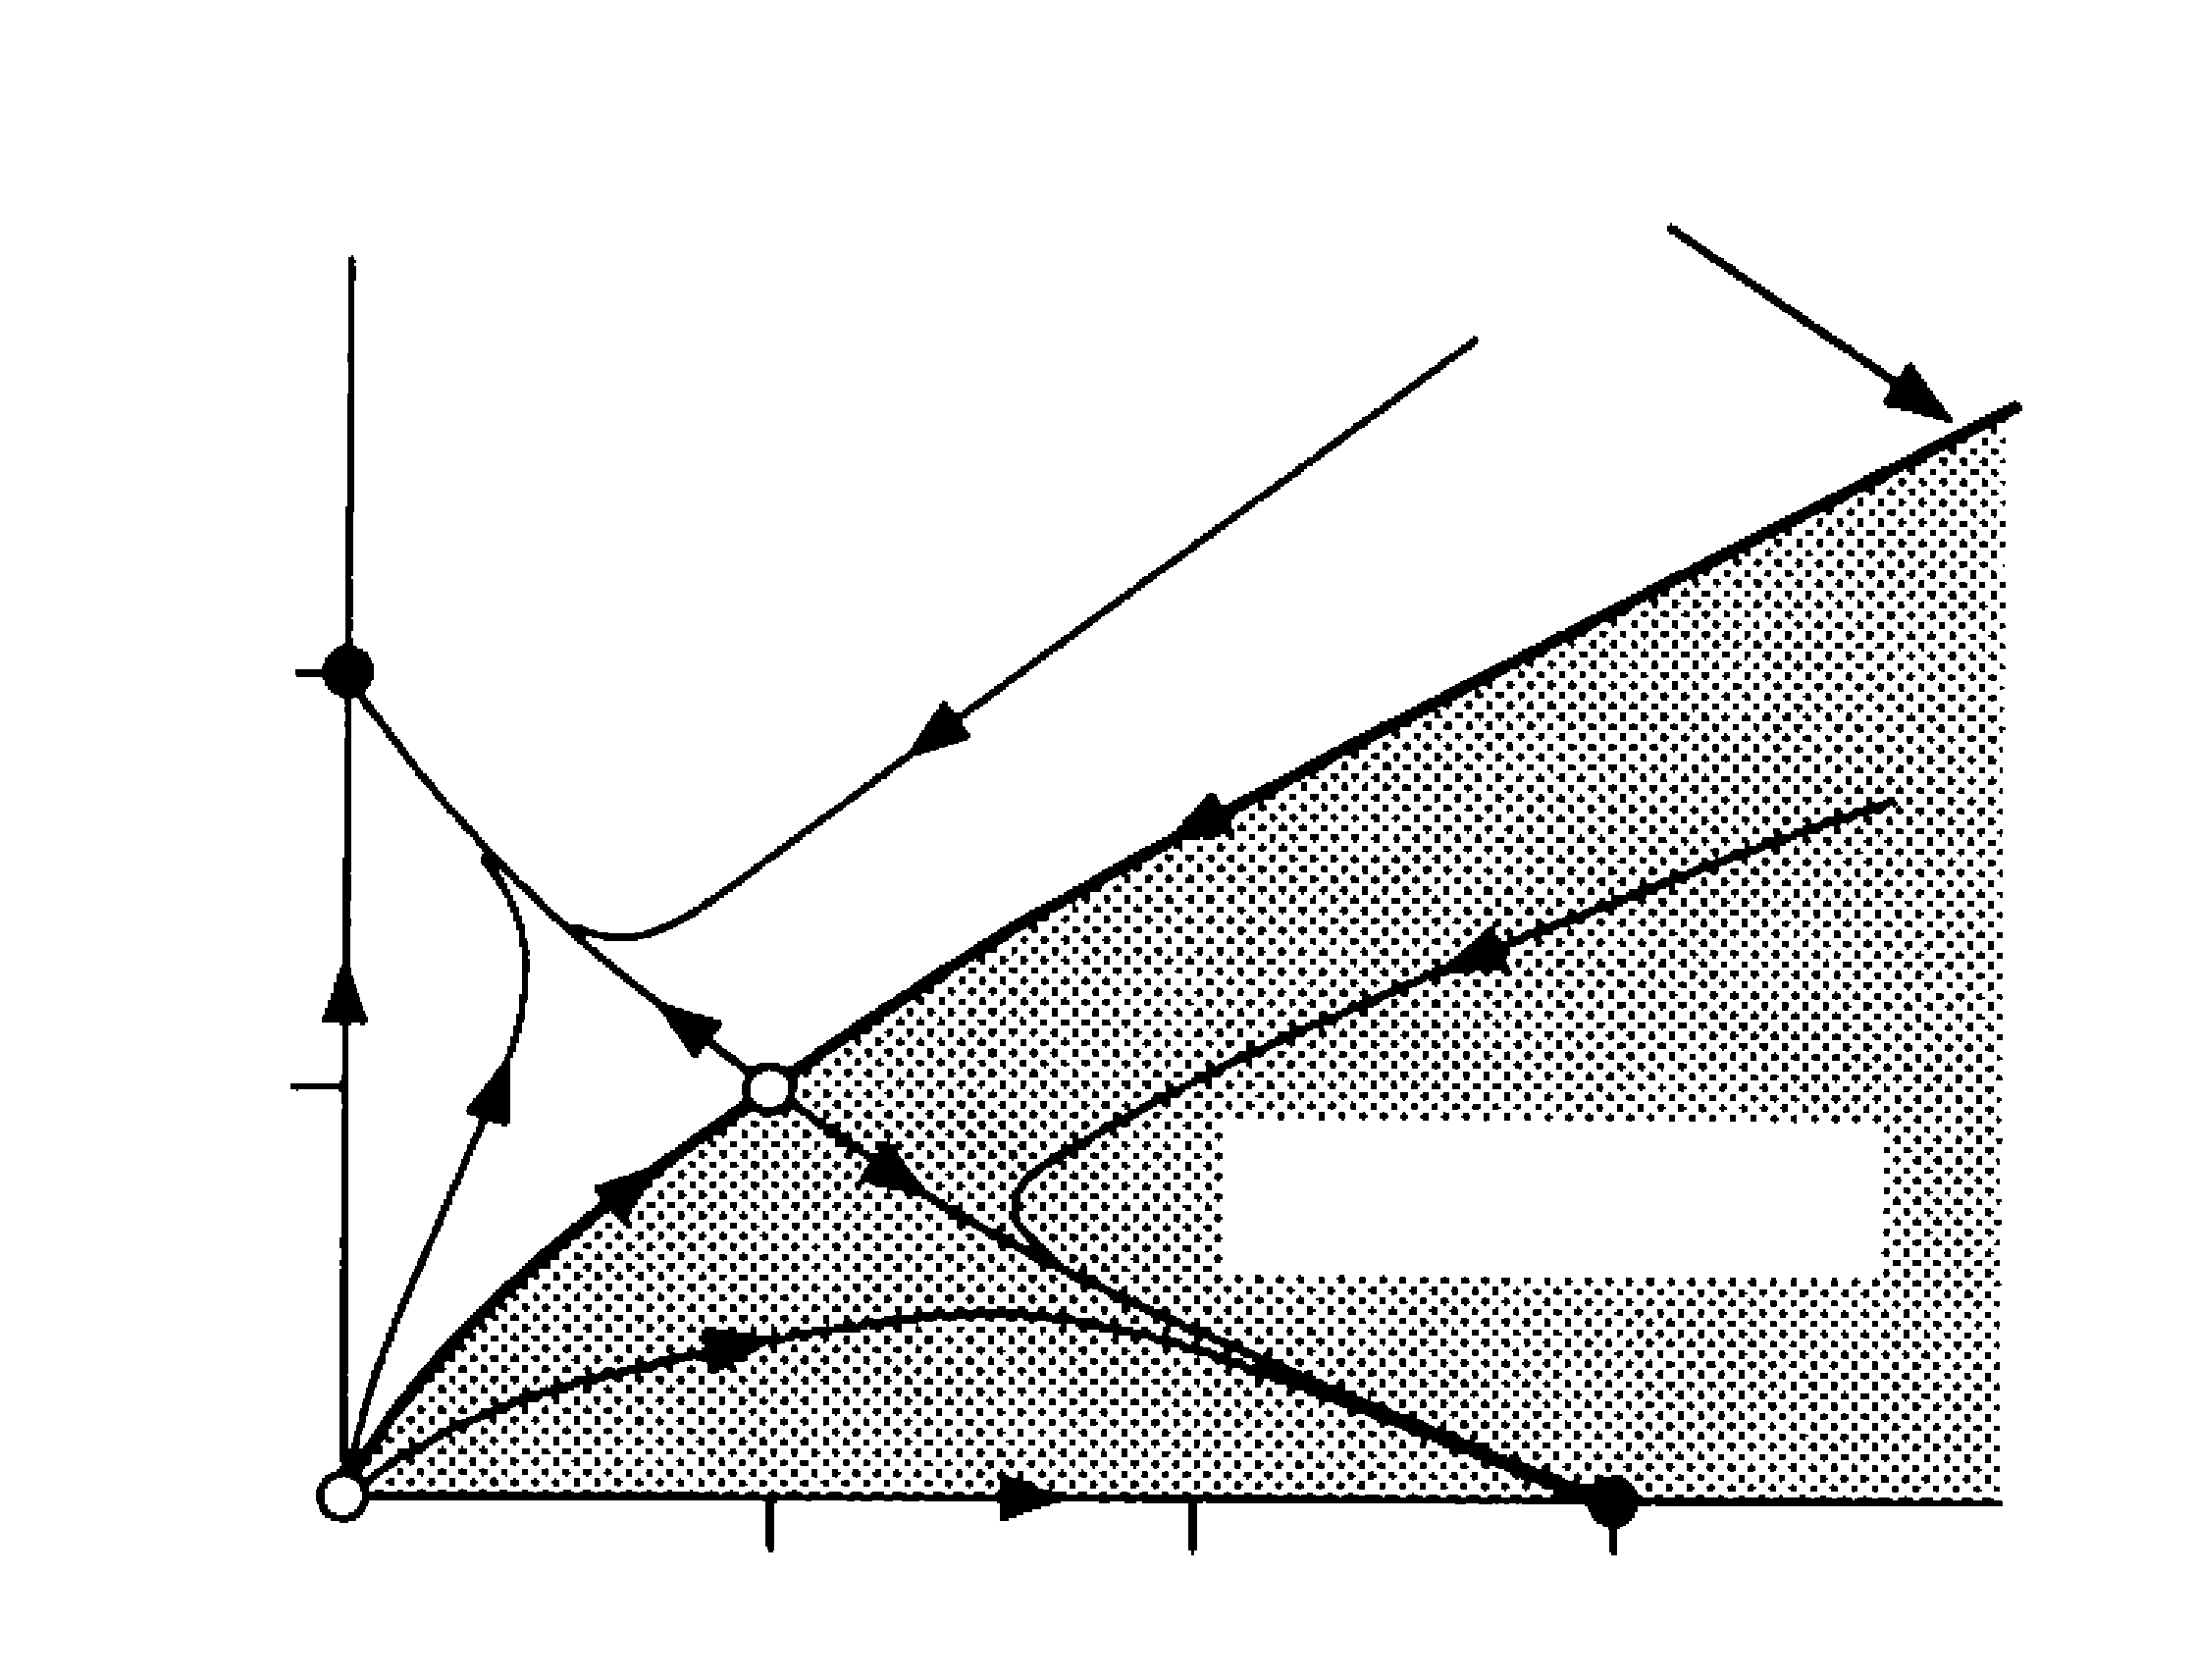
\includegraphics[width=0.82\textwidth]{images/Figures/figur-016.png}
\caption{$(3,0)$ noktasının çekim havzası ve havza sınırı.}
\label{fig:6-4-8}
\end{figure}
\end{justify}

\newpage
\section{Korunumlu Sistemler}

\begin{justify}
Newton yasası $F=ma$, birçok önemli ikinci mertebeden sistemin kaynağıdır. $x$ ekseni boyunca hareket eden ve doğrusal olmayan $F(x)$ kuvvetine maruz kalan $m$ kütleli parçacık için
\begin{equation}
m\ddot{x}=F(x)
\end{equation}
yazılır. Kuvvet hızdan ve zamandan bağımsızsa sönüm ya da dış zorlama yoktur.

$V(x)$ potansiyel enerji olsun ve
\begin{equation}
F(x)=-\frac{dV}{dx}
\end{equation}
ile tanımlansın. Böylece
\begin{equation}
m\ddot{x}+\frac{dV}{dx}=0
\end{equation}
olur. Denklem $\dot{x}$ ile çarpılırsa
\begin{equation}
\frac{d}{dt}\left[\frac{1}{2}m\dot{x}^{2}+V(x)\right]=0
\end{equation}
elde edilir. Dolayısıyla toplam enerji
\begin{equation}
E=\frac{1}{2}m\dot{x}^{2}+V(x)
\end{equation}
zaman boyunca sabittir. Korunan büyüklüğe sahip sistemlere korunumlu sistemler denir.
\end{justify}

\subsection*{Örnek 6.5.1}
\addcontentsline{toc}{subsection}{Örnek 6.5.1}

\begin{justify}
Korunumlu bir sistemin çekici sabit noktaya sahip olamayacağını gösterelim. $\mathbf{x}^{*}$ çekici sabit nokta olsaydı, çekim havzasındaki tüm noktalar aynı enerjiye sahip olurdu. Bu durumda $E(\mathbf{x})$ havza içinde sabit olurdu; bu da korunumlu sistem tanımıyla çelişir.
\end{justify}

\subsection*{Örnek 6.5.2}
\addcontentsline{toc}{subsection}{Örnek 6.5.2}

\begin{justify}
Kütlesi $m=1$ olan ve çift kuyulu potansiyel
\begin{equation}
V(x)=-\frac{1}{2}x^2+\frac{1}{4}x^4
\end{equation}
içinde hareket eden parçacığı ele alalım. Kuvvet
\begin{equation}
F=-\frac{dV}{dx}=x-x^3
\end{equation}
olduğundan
\begin{equation}
\ddot{x}=x-x^3
\end{equation}
yazılır. Vektör alanı
\begin{align}
\dot{x} &= y,\\
\dot{y} &= x-x^3
\end{align}
şeklindedir. Denge noktaları $(0,0)$ ve $(\pm1,0)$ noktalarıdır. Jacobian
\begin{equation}
A=\begin{pmatrix}0&1\\1-3x^2&0\end{pmatrix}
\end{equation}
olur. Orijin eyer noktasıdır; $(\pm1,0)$ noktaları merkez olarak öngörülür.

Enerji korunumu nedeniyle yörüngeler sabit enerji konturlarıdır:
\begin{equation}
E=\frac{1}{2}y^2-\frac{1}{2}x^2+\frac{1}{4}x^4=\text{sabit}.
\end{equation}
Faz portresi Şekil~\ref{fig:6-5-1}'de, fiziksel çift kuyu yorumu Şekil~\ref{fig:6-5-2}'de gösterilecektir.
\begin{figure}[H]
\centering
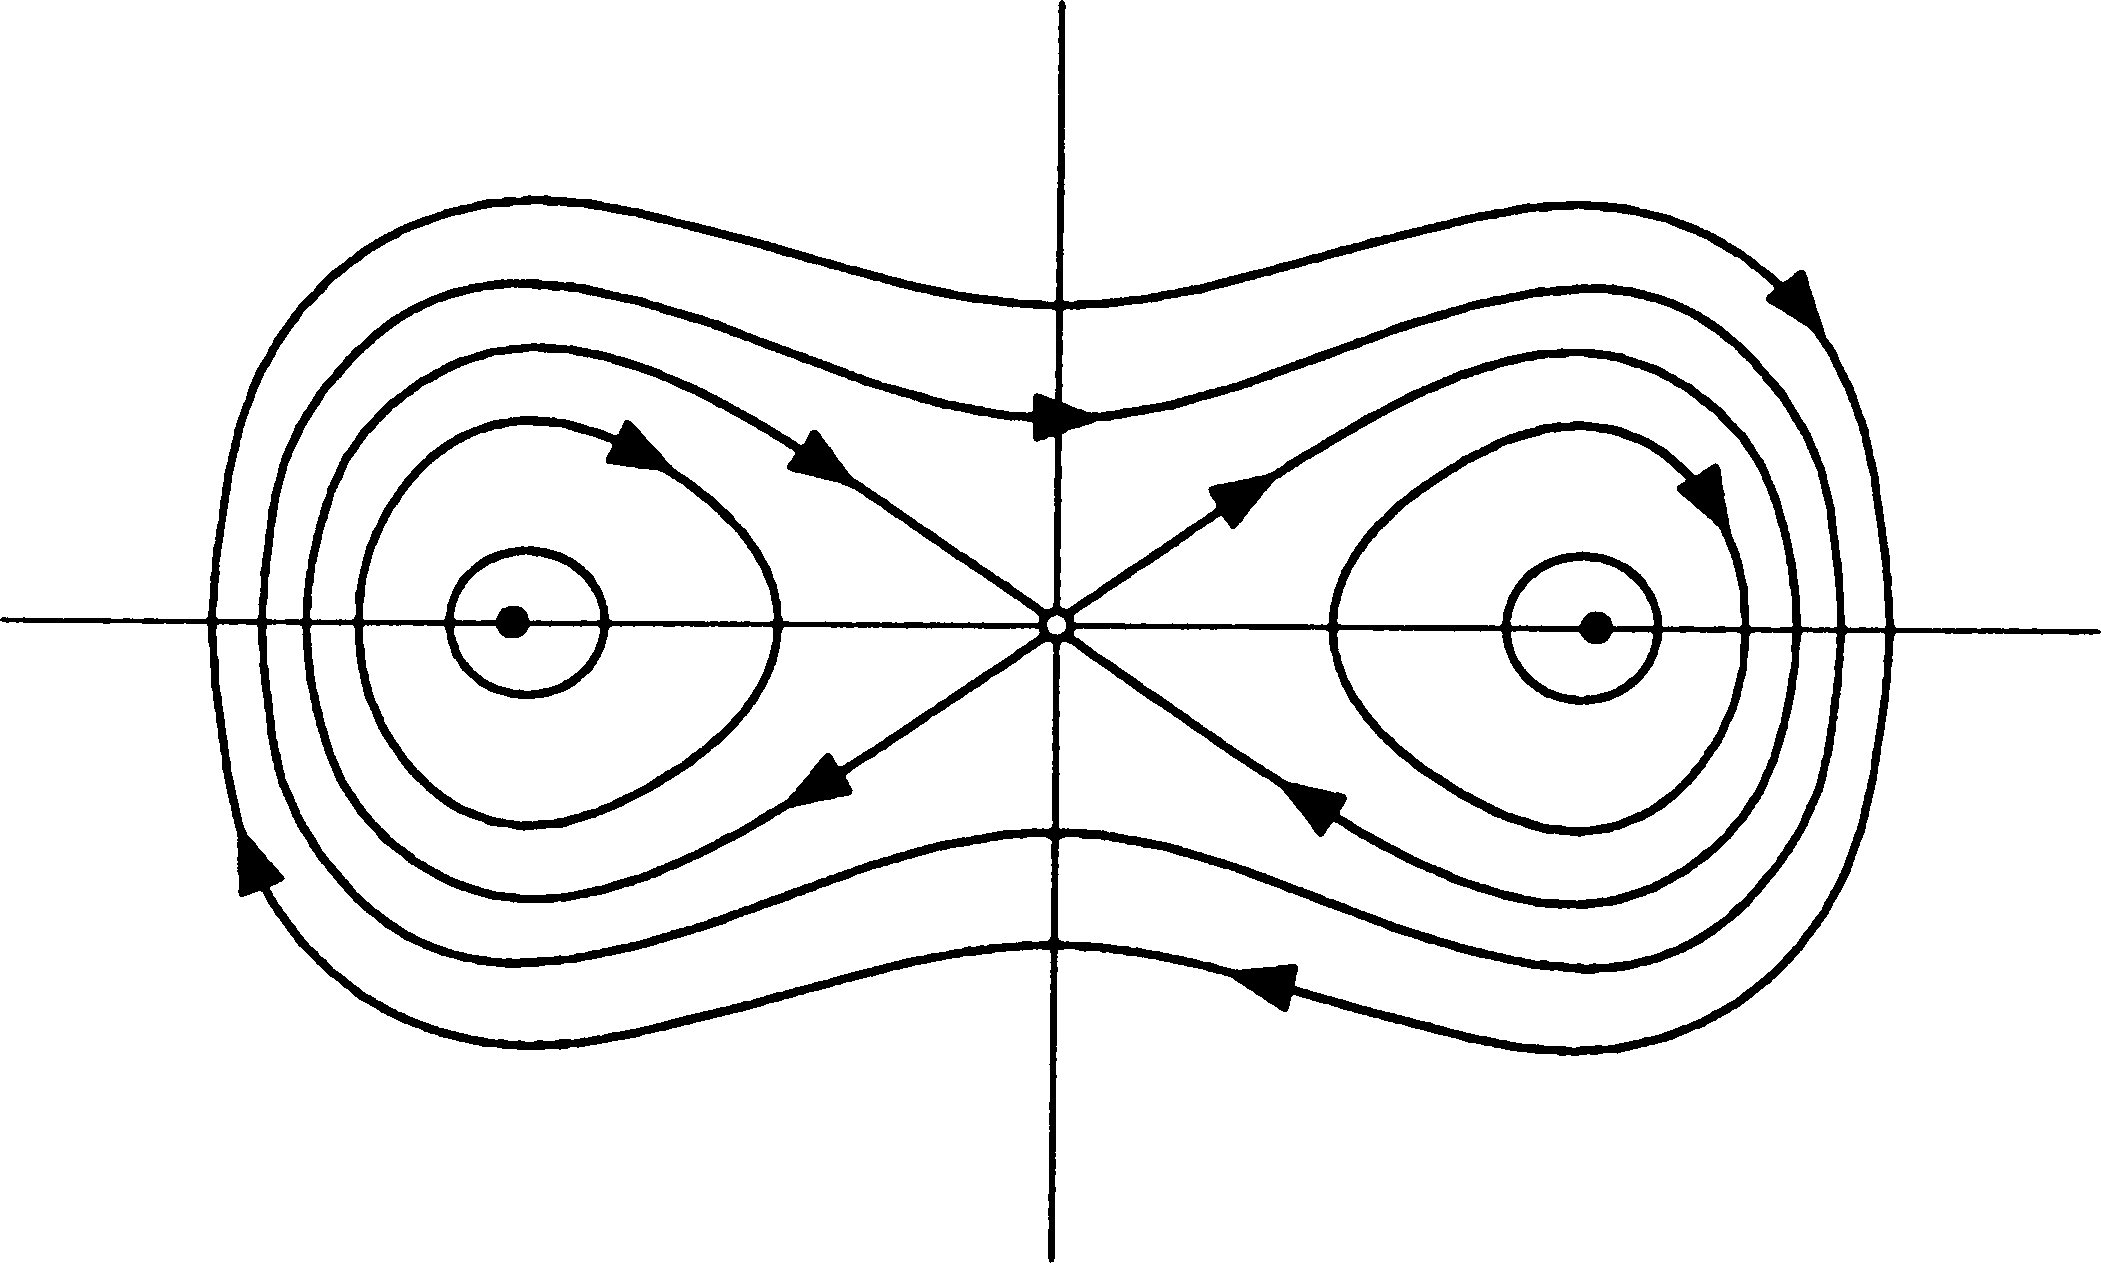
\includegraphics[width=0.82\textwidth]{images/Figures/figur-018.png}
\caption{Çift kuyulu potansiyel için faz portresi ve sabit enerji eğrileri.}
\label{fig:6-5-1}
\end{figure}
\begin{figure}[H]
\centering
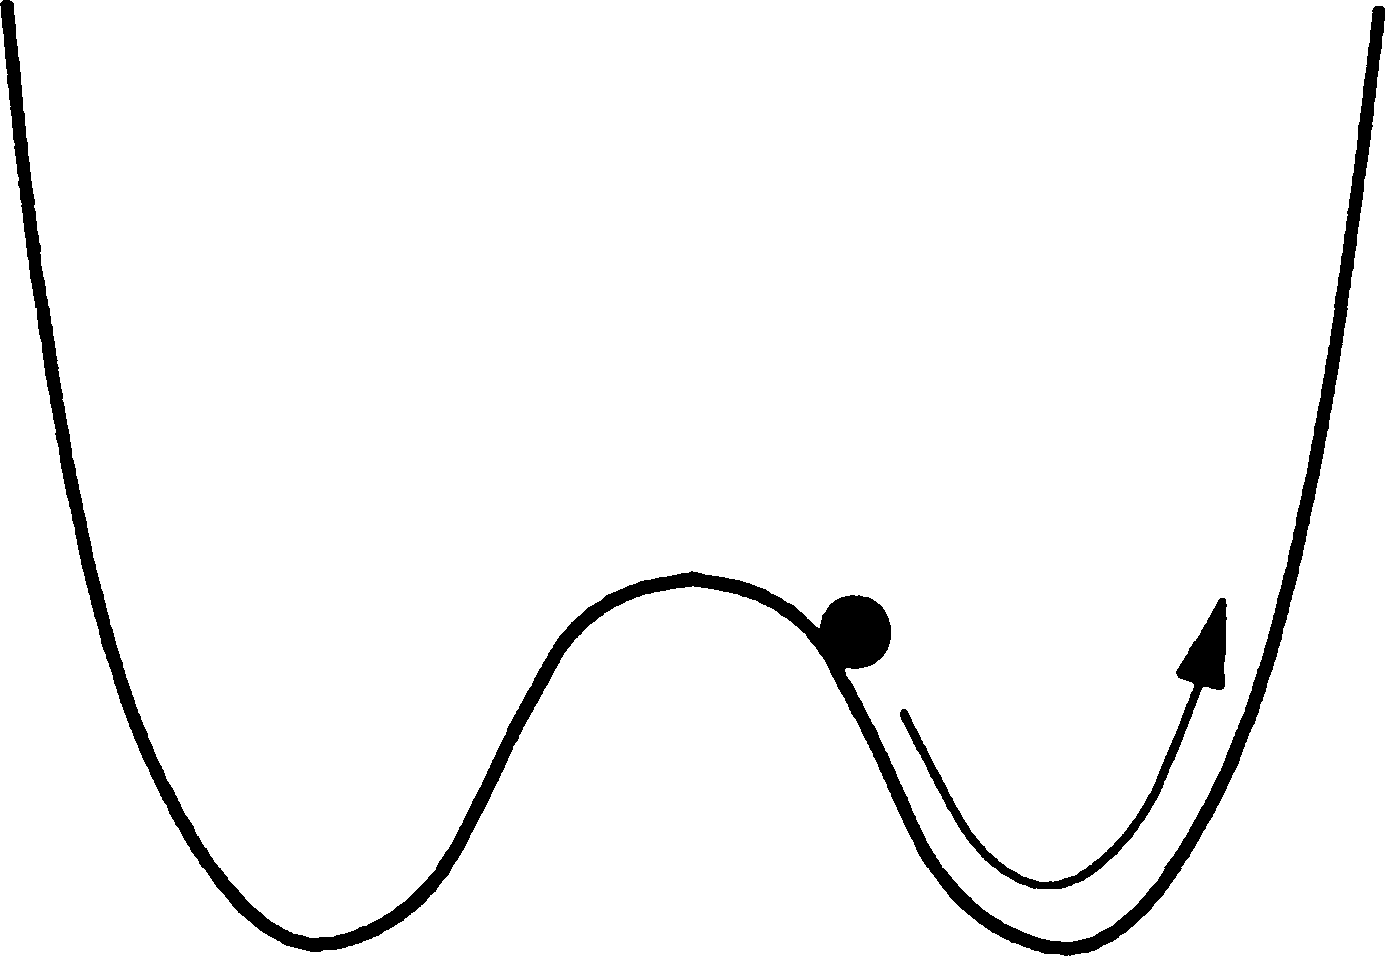
\includegraphics[width=0.82\textwidth]{images/Figures/figur-017.png}
\caption{Çift kuyulu potansiyelde parçacığın fiziksel hareketi.}
\label{fig:6-5-2}
\end{figure}
\end{justify}

\subsection*{Örnek 6.5.3}
\addcontentsline{toc}{subsection}{Örnek 6.5.3}

\begin{justify}
Örnek 6.5.2 için enerji fonksiyonu $E(x,y)$'nin grafiği enerji yüzeyi olarak adlandırılır (Şekil~\ref{fig:6-5-3}). Yerel minimumlar faz düzleminde merkezlere karşılık gelir.
\begin{figure}[H]
\centering
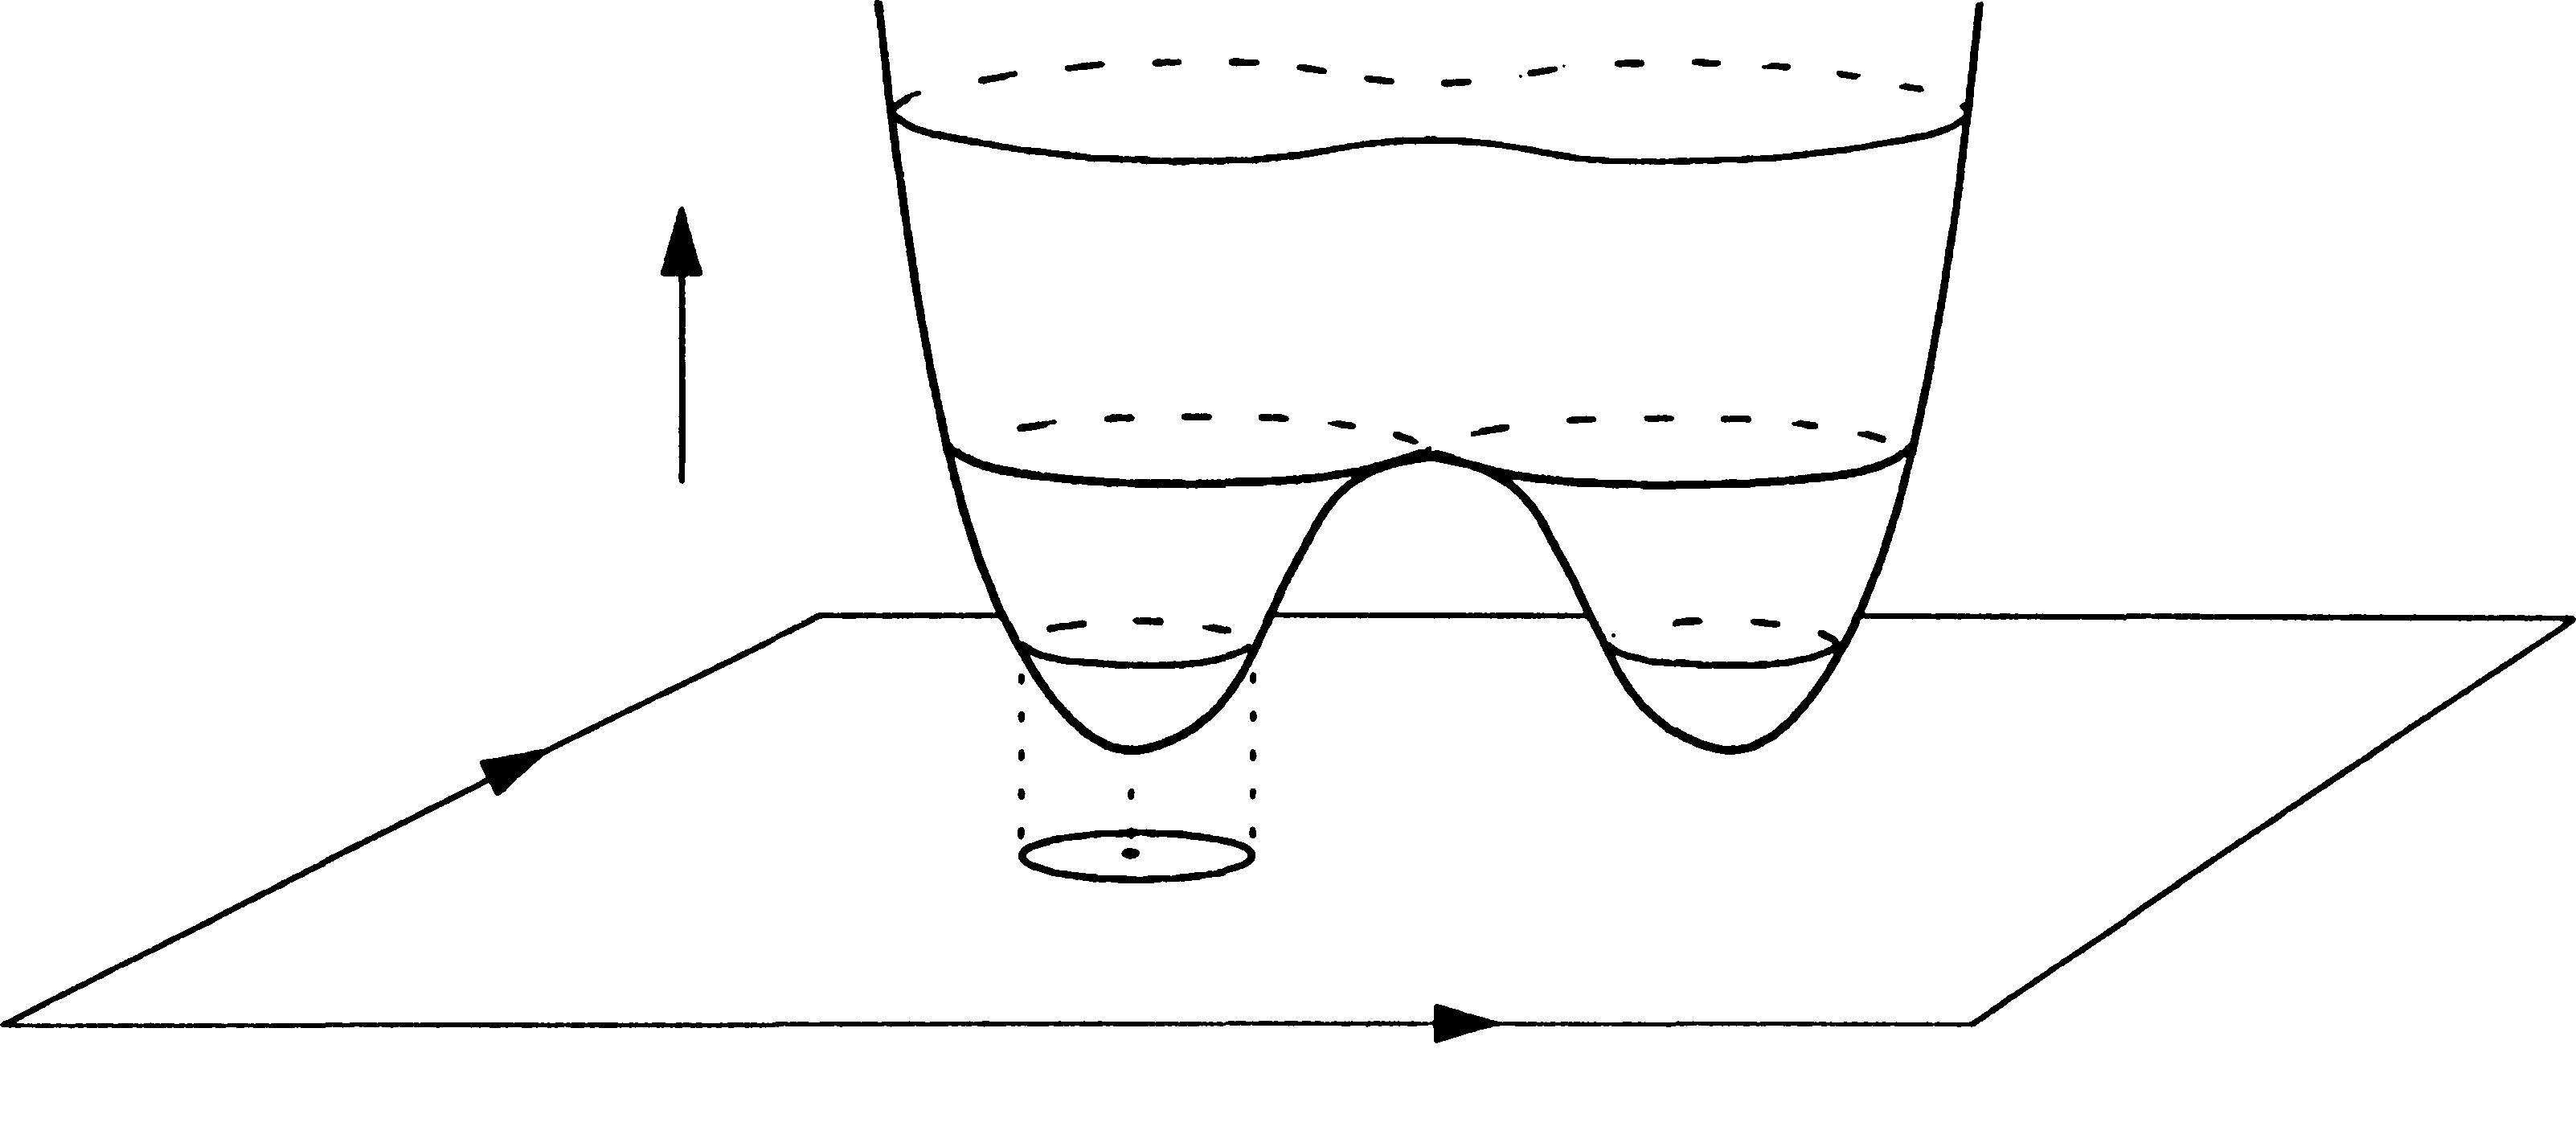
\includegraphics[width=0.82\textwidth]{images/Figures/figur-019.png}
\caption{Örnek 6.5.2 için enerji yüzeyi.}
\label{fig:6-5-3}
\end{figure}
\end{justify}

\subsection*{Doğrusal Olmayan Merkezler}
\addcontentsline{toc}{subsection}{Doğrusal Olmayan Merkezler}

\begin{justify}
Korunumlu sistemlerde merkezler daha dayanıklıdır; çünkü yörüngeler enerji konturları üzerinde kalır. Eğer izole bir sabit nokta $\mathbf{x}^{*}$, korunan büyüklük $E(\mathbf{x})$ için yerel minimum ise, $\mathbf{x}^{*}$ noktasına yeterince yakın tüm yörüngeler kapalıdır. Bu nedenle $\mathbf{x}^{*}$ doğrusal olmayan bir merkezdir.
\end{justify}

\newpage
\section{Tersinir Sistemler}

\begin{justify}
Birçok mekanik sistem zaman tersinim simetrisine sahiptir. Bu, zaman ileri ya da geri aksa da sistemin dinamiğinin aynı görünmesi anlamına gelir. Örneğin sönümsüz bir sarkacın ileri geri salındığı bir filmi geriye doğru izlerseniz fiziksel olarak saçma bir durum görmezsiniz.

Aslında
\begin{equation}
m\ddot{x}=F(x)
\end{equation}
biçimindeki her mekanik sistem zaman tersinimi altında simetriktir. $t\mapsto -t$ değişken dönüşümü yapılırsa ikinci türev $\ddot{x}$ değişmez ve denklem aynı kalır. Elbette hız $\dot{x}$ işaret değiştirir. Bunun faz düzleminde ne anlama geldiğini görmek için eşdeğer sistemi yazalım:
\begin{align}
\dot{x} &= y,\\
\dot{y} &= \frac{1}{m}F(x),
\end{align}
burada $y$ hızdır. $t\mapsto -t$ ve $y\mapsto -y$ dönüşümleri yapılırsa iki denklem de aynı kalır. Dolayısıyla $(x(t),y(t))$ bir çözümse, $(x(-t),-y(-t))$ de bir çözümdür. Bu nedenle her yörüngenin bir ikizi vardır: bu iki yörünge yalnızca zamanın ters çevrilmesi ve $x$ eksenine göre yansıma bakımından farklıdır (Şekil~\ref{fig:6-6-1}).

\begin{figure}[H]
\centering
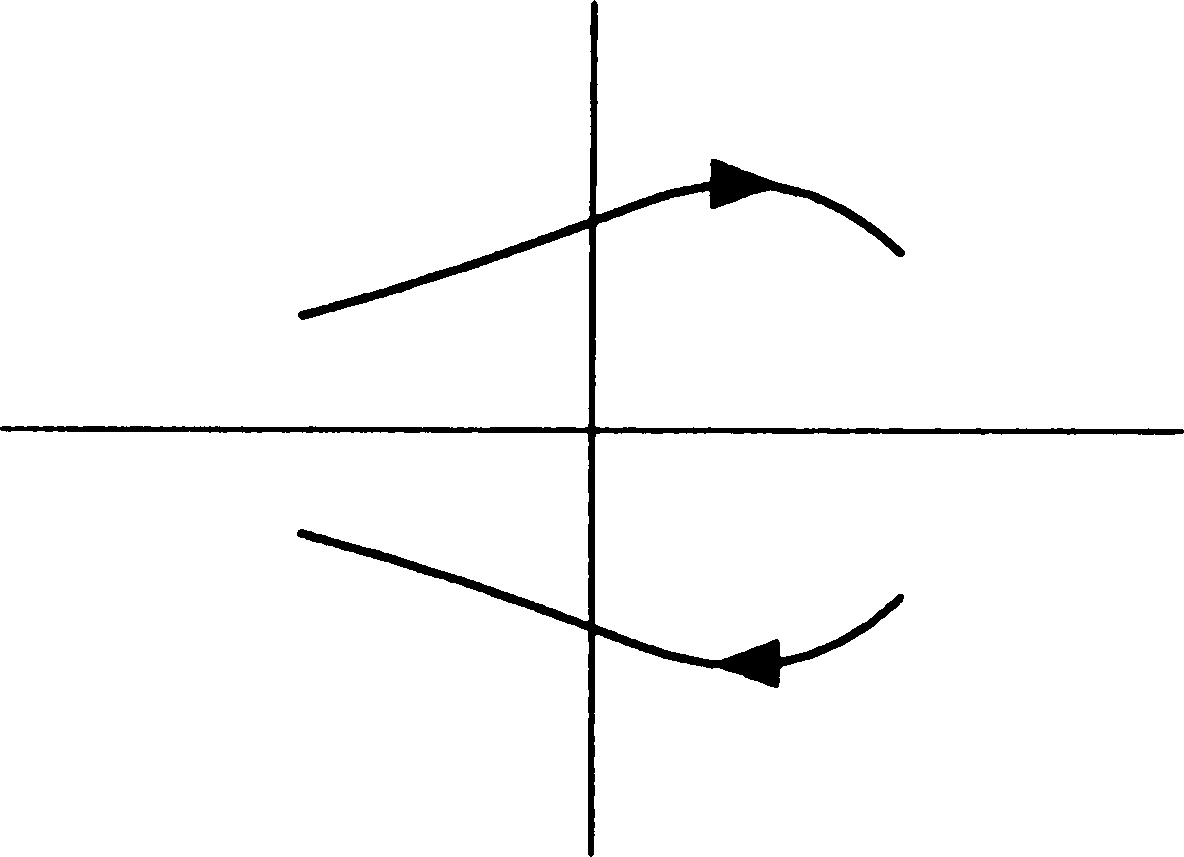
\includegraphics[width=0.82\textwidth]{images/Figures/figur-020.png}
\caption{Tersinir sistemde yörüngenin $x$ eksenine göre yansıyan ikizi.}
\label{fig:6-6-1}
\end{figure}

Genel olarak, $t\mapsto -t$ ve $y\mapsto -y$ altında değişmeyen her ikinci mertebeden sistemi tersinir sistem olarak tanımlayalım. Örneğin
\begin{align}
\dot{x} &= f(x,y),\\
\dot{y} &= g(x,y)
\end{align}
biçimindeki bir sistemde $f$ fonksiyonu $y$ değişkenine göre tek, $g$ fonksiyonu ise $y$ değişkenine göre çift ise sistem tersinirdir; yani
\begin{equation}
f(x,-y)=-f(x,y), \qquad g(x,-y)=g(x,y).
\end{equation}

Tersinir sistemler korunumlu sistemlerden farklıdır; fakat onların birçok özelliğine sahiptir. Örneğin aşağıdaki teorem, merkezlerin tersinir sistemlerde de dayanıklı olduğunu gösterir.

\textbf{Teorem 6.6.1.} Orijin, sürekli türevlenebilir
\begin{align}
\dot{x} &= f(x,y),\\
\dot{y} &= g(x,y)
\end{align}
sistemi için doğrusal bir merkez olsun ve sistem tersinir olsun. O zaman orijine yeterince yakın tüm yörüngeler kapalı eğrilerdir.

\textbf{İspat fikri.} Orijine yakın pozitif $x$ ekseni üzerinde başlayan bir yörünge düşünelim (Şekil~\ref{fig:6-6-2}). Orijine yeterince yakın bölgede doğrusal merkezin baskın etkisi nedeniyle akış orijin çevresinde döner ve yörünge sonunda negatif $x$ eksenini keser. Şimdi tersinirlik kullanılır. Yörünge $x$ eksenine göre yansıtılır ve zamanın işareti değiştirilirse, aynı uç noktalara sahip fakat oku ters yönde olan ikiz bir yörünge elde edilir (Şekil~\ref{fig:6-6-3}). Bu iki yörünge birlikte kapalı bir yörünge oluşturur.

\begin{figure}[H]
\centering
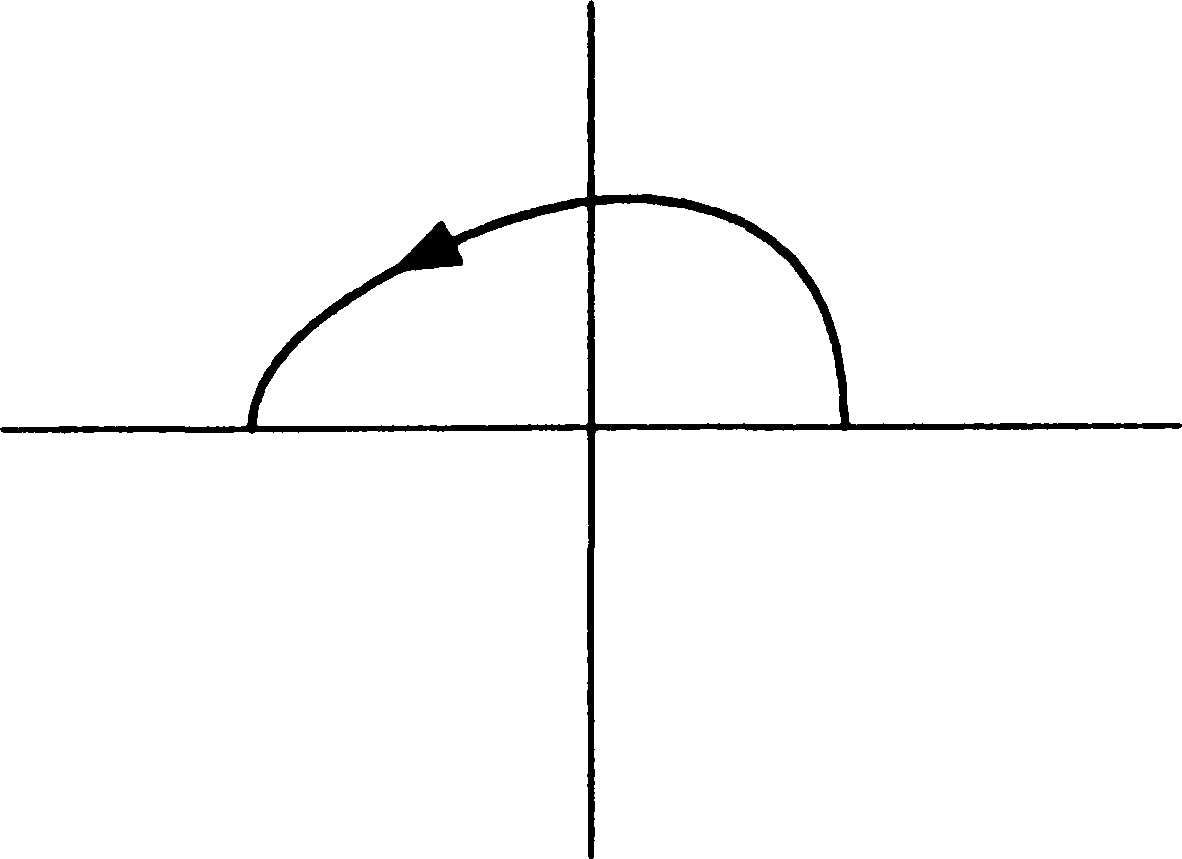
\includegraphics[width=0.82\textwidth]{images/Figures/figur-021.png}
\caption{Pozitif $x$ ekseninden başlayan yörüngenin negatif $x$ eksenini kesmesi.}
\label{fig:6-6-2}
\end{figure}
\begin{figure}[H]
\centering
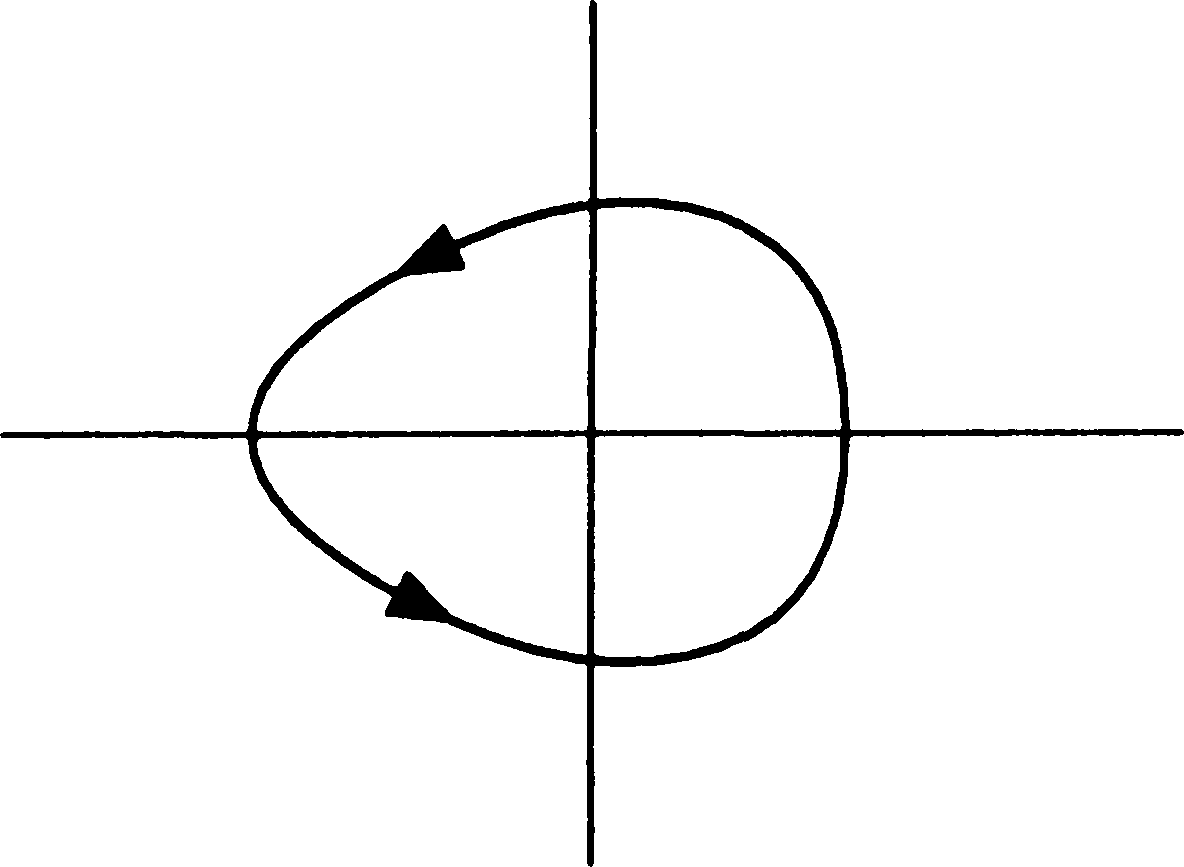
\includegraphics[width=0.82\textwidth]{images/Figures/figur-022.png}
\caption{Tersinirlik ile elde edilen ikiz yörünge ve kapalı eğri.}
\label{fig:6-6-3}
\end{figure}
\end{justify}

\subsection*{Örnek 6.6.1}
\addcontentsline{toc}{subsection}{Örnek 6.6.1}

\begin{justify}
Aşağıdaki sistemin orijinde doğrusal olmayan bir merkeze sahip olduğunu gösterin ve faz portresini çizin:
\begin{align}
\dot{x} &= y-y^3,\\
\dot{y} &= -x-y^2.
\end{align}

\textbf{Çözüm.} Teoremin varsayımlarının sağlandığını göstereceğiz. Orijindeki Jacobian matrisi
\begin{equation}
A=\begin{pmatrix}0&1\\-1&0\end{pmatrix}
\end{equation}
olur. Bu matris için $\tau=0$ ve $\Delta>0$ olduğundan orijin doğrusal bir merkezdir. Ayrıca sistem $t\mapsto -t$, $y\mapsto -y$ dönüşümü altında değişmediği için tersinirdir. Teorem 6.6.1'e göre orijin doğrusal olmayan bir merkezdir.

Sistemin diğer sabit noktaları $(-1,1)$ ve $(-1,-1)$ noktalarıdır. Lineerleştirme ile kolayca kontrol edilebileceği gibi bunlar eyer noktalarıdır. Bilgisayar üretimli faz portresi Şekil~\ref{fig:6-6-4}'te gösterilecektir. Tersinirlik simetrisi açıktır: $x$ ekseninin üstündeki yörüngelerin, okları ters yönde olacak şekilde altında ikizleri bulunur.

\begin{figure}[H]
\centering
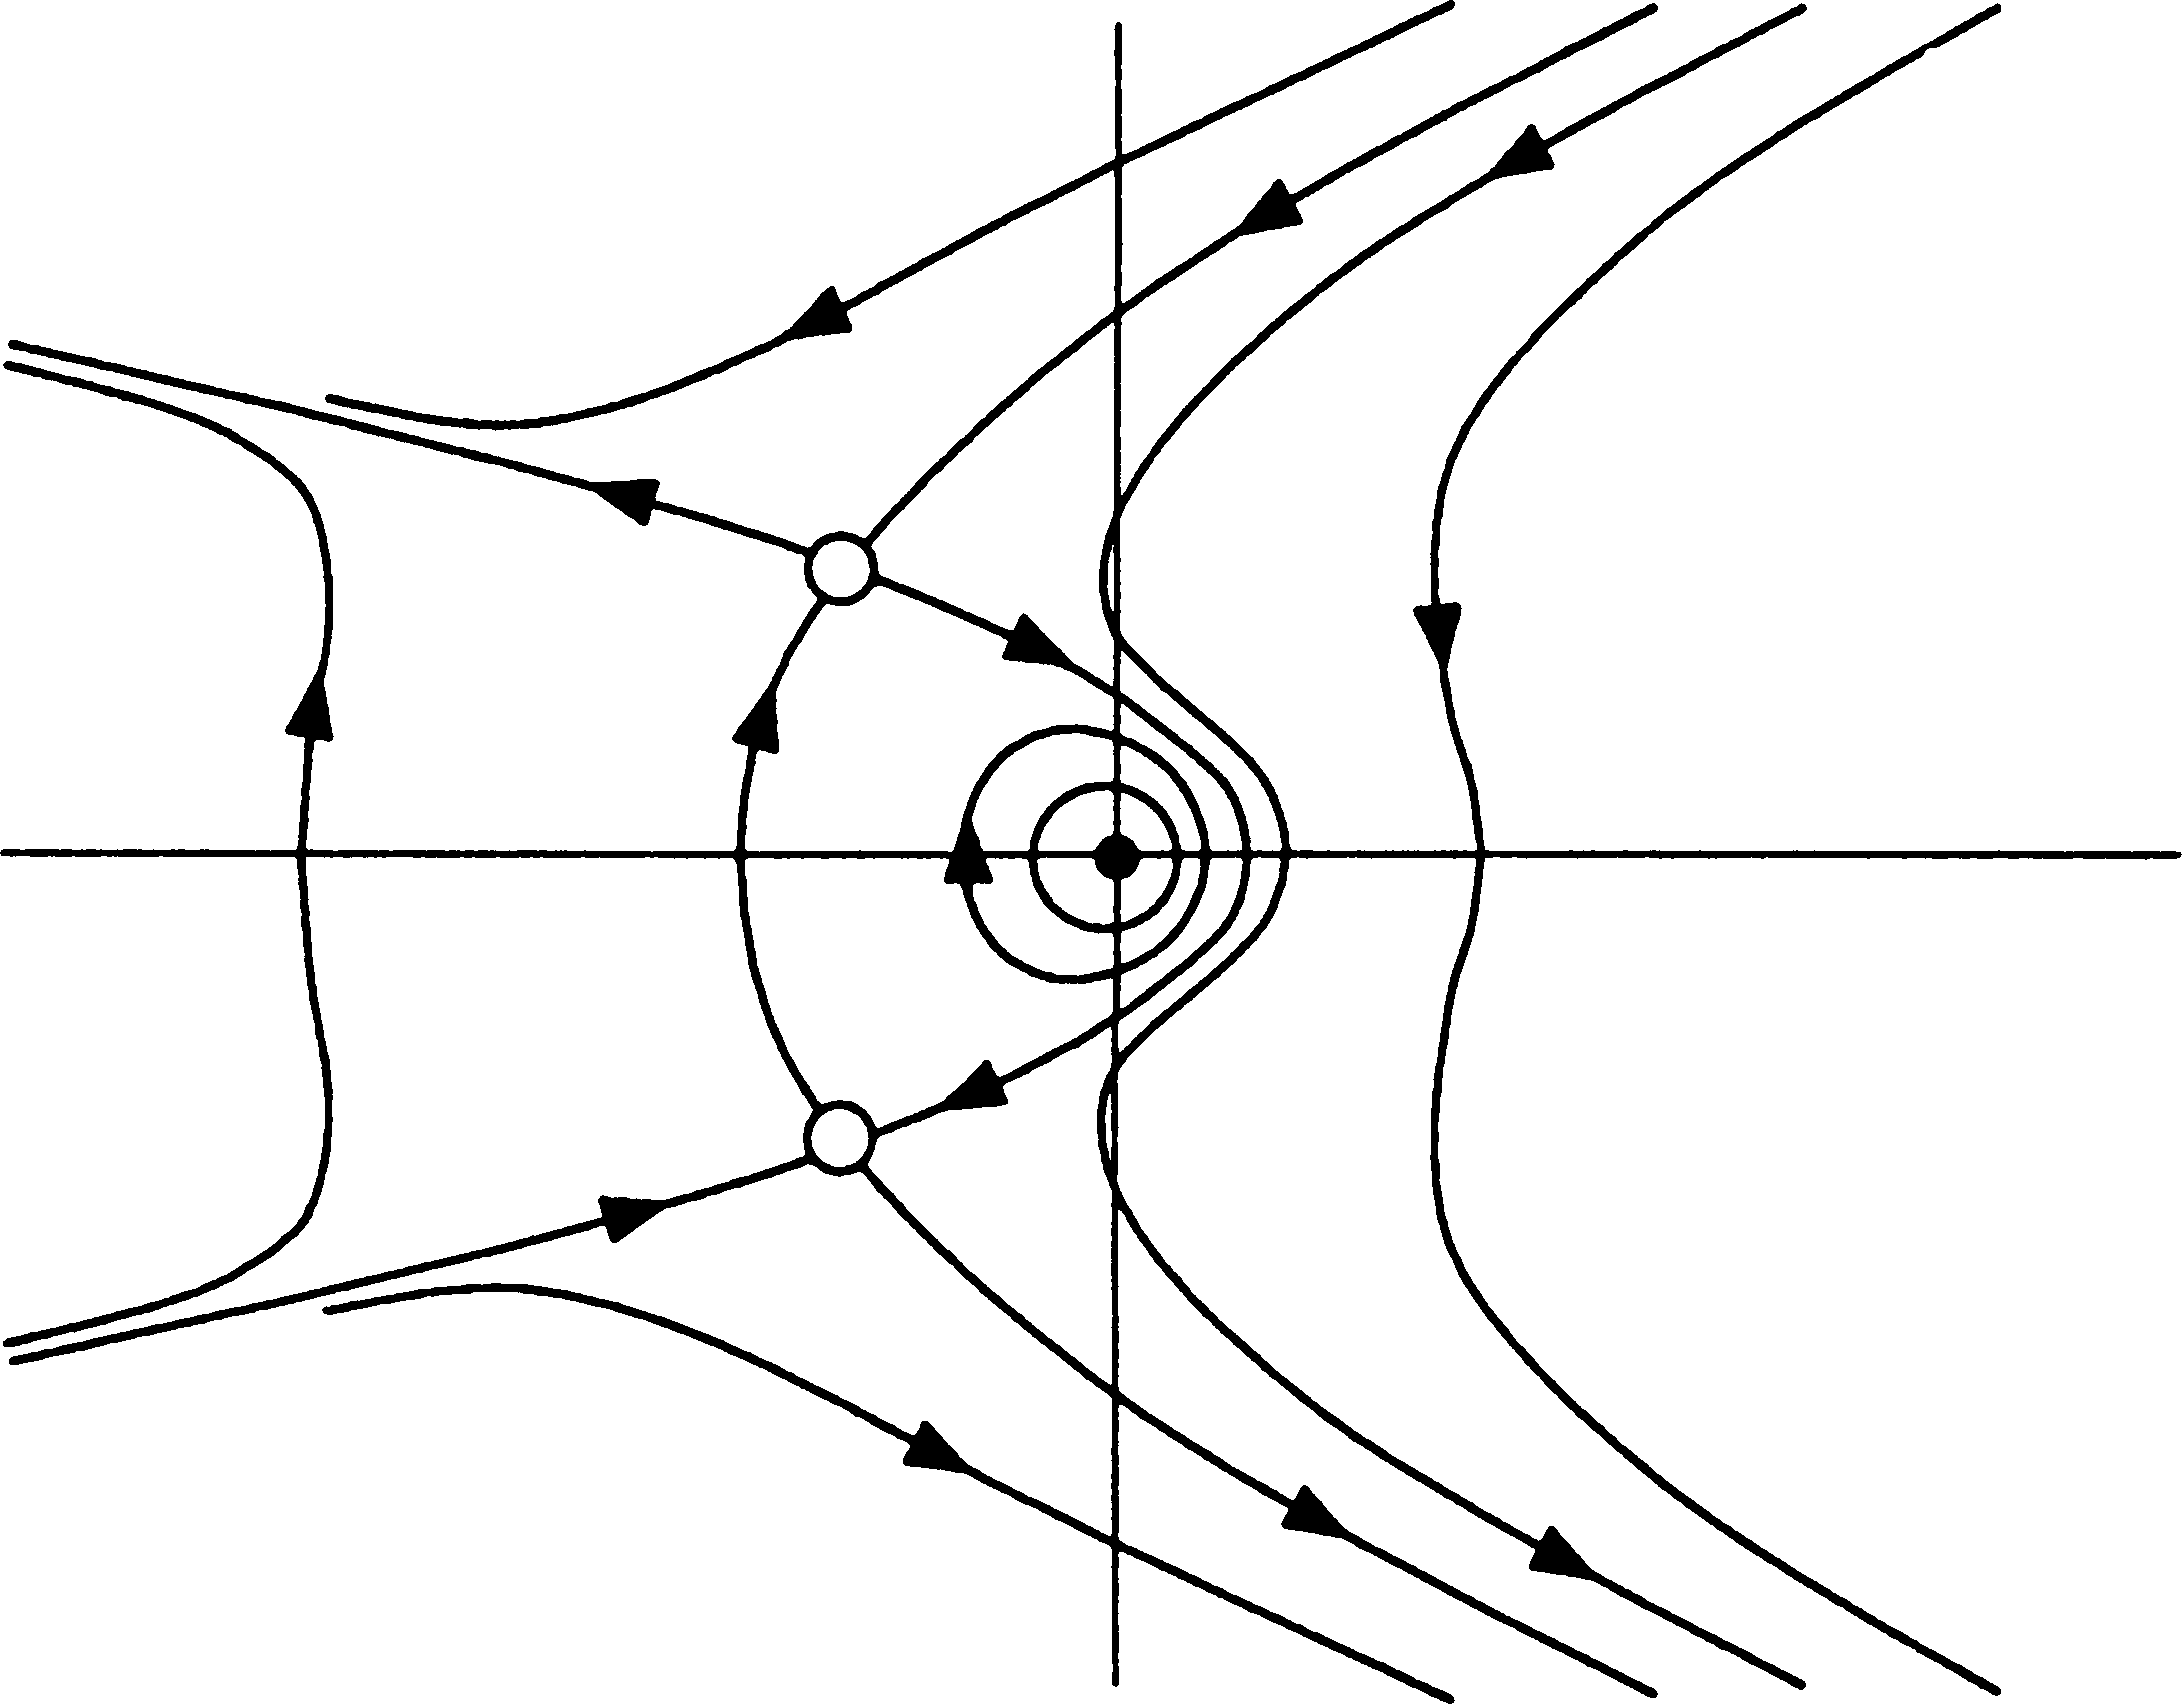
\includegraphics[width=0.82\textwidth]{images/Figures/figur-023.png}
\caption{Örnek 6.6.1 için tersinir sistemin faz portresi.}
\label{fig:6-6-4}
\end{figure}

İkiz eyer noktalarının bir yörünge çiftiyle bağlandığına dikkat ediniz. Bunlara heteroklinik yörüngeler ya da eyer bağlantıları denir. Homoklinik yörüngeler gibi, heteroklinik yörüngeler de tersinir veya korunumlu sistemlerde diğer sistemlere göre çok daha yaygındır.
\end{justify}

\subsection*{Örnek 6.6.2}
\addcontentsline{toc}{subsection}{Örnek 6.6.2}

\begin{justify}
Yalnızca tersinirlik argümanlarını kullanarak
\begin{align}
\dot{x} &= y,\\
\dot{y} &= x-x^2
\end{align}
sisteminin $x\ge 0$ yarı düzleminde bir homoklinik yörüngeye sahip olduğunu gösterelim.

\textbf{Çözüm.} Orijindeki eyer noktasının kararsız manifoldunu ele alalım. Lineerleştirme için kararsız özdoğrultu $(1,1)$ olduğundan, bu manifold orijini bu doğrultu boyunca terk eder. Bu nedenle orijine yakın bölgede kararsız manifoldun bir parçası birinci bölgede, yani $x,y>0$ bölgesinde yer alır.

Başlangıçta $\dot{x}=y>0$ olduğundan $x(t)$ artar. Ayrıca küçük $x$ için $\dot{y}=x-x^2>0$ olduğundan $y(t)$ de başlangıçta artar. Böylece faz noktası yukarı ve sağa doğru hareket eder. Yatay hızı artmaya devam ettiği için bir zamanda $x=1$ doğrusunu keser. Bundan sonra $\dot{y}<0$ olur ve $y(t)$ azalır; sonunda $y=0$ değerine ulaşır (Şekil~\ref{fig:6-6-5}).

Tersinirlik nedeniyle aynı uç noktalara sahip fakat oku ters yönde olan ikiz bir yörünge bulunmalıdır (Şekil~\ref{fig:6-6-6}). Bu iki yörünge birlikte istenen homoklinik yörüngeyi oluşturur.

\begin{figure}[H]
\centering
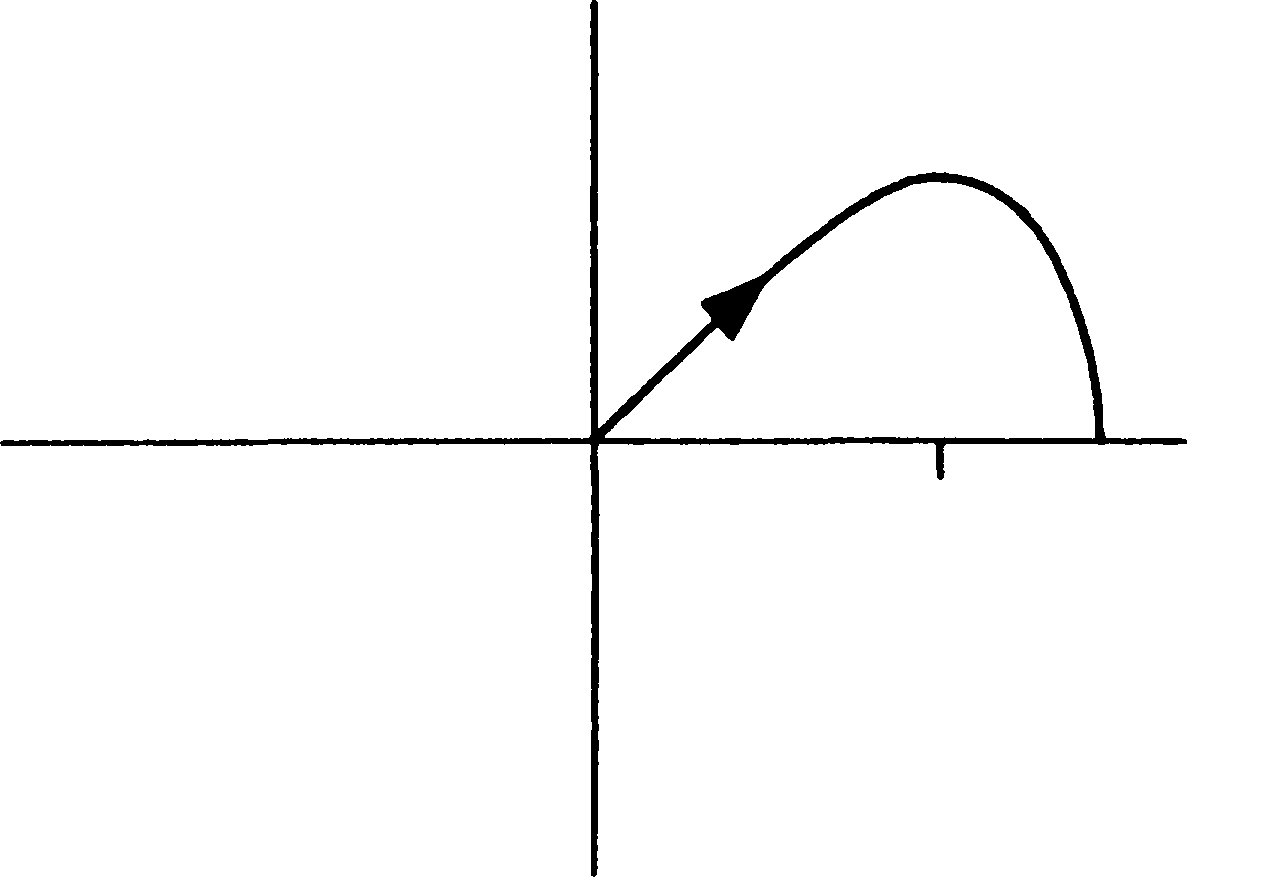
\includegraphics[width=0.82\textwidth]{images/Figures/figur-024.png}
\caption{Kararsız manifoldun $x=1$ doğrusunu kesip $y=0$ eksenine ulaşması.}
\label{fig:6-6-5}
\end{figure}
\begin{figure}[H]
\centering
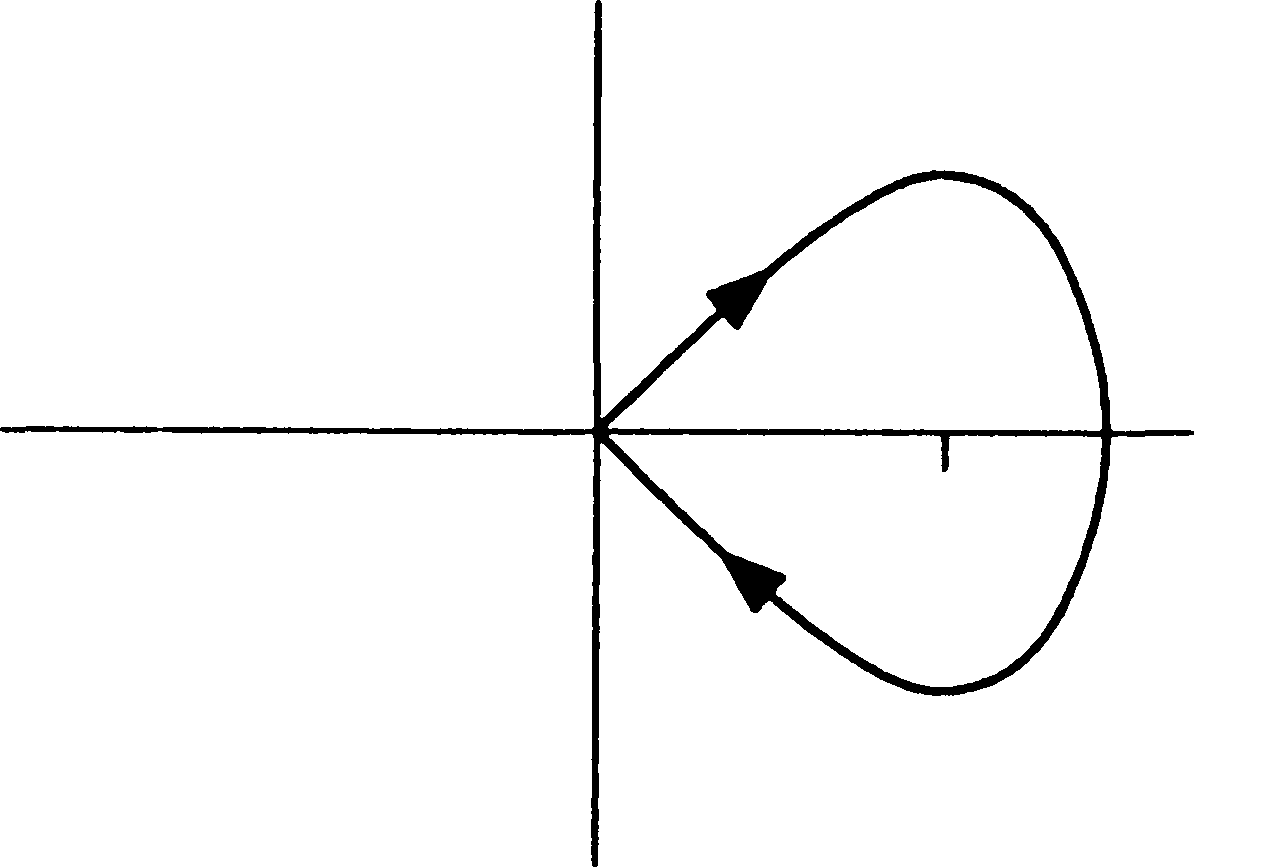
\includegraphics[width=0.82\textwidth]{images/Figures/figur-025.png}
\caption{Tersinirlik ile tamamlanan homoklinik yörünge.}
\label{fig:6-6-6}
\end{figure}
\end{justify}

\subsection*{Örnek 6.6.3}
\addcontentsline{toc}{subsection}{Örnek 6.6.3}

\begin{justify}
Aşağıdaki sistemin tersinir fakat korunumlu olmadığını gösterelim ve faz portresini çizelim:
\begin{align}
\dot{x} &= -2\cos x-\cos y,\\
\dot{y} &= -2\cos y-\cos x.
\end{align}

\textbf{Çözüm.} Sistem $t\mapsto -t$, $x\mapsto -x$ ve $y\mapsto -y$ değişken dönüşümleri altında değişmez. Bu nedenle $R(x,y)=(-x,-y)$ dönüşümüyle tersinirdir.

Sistemin korunumlu olmadığını göstermek için çekici bir sabit noktasının olduğunu göstermek yeterlidir. Sabit noktalar
\begin{equation}
2\cos x=-\cos y, \qquad 2\cos y=-\cos x
\end{equation}
koşullarını sağlar. Bu denklemler birlikte çözülünce $\cos x^{*}=\cos y^{*}=0$ bulunur. Böylece dört sabit nokta vardır:
\begin{equation}
(x^{*},y^{*})=\left(\pm\frac{\pi}{2},\pm\frac{\pi}{2}\right).
\end{equation}
$(-\pi/2,-\pi/2)$ noktasının çekici olduğunu gösterelim. Bu noktadaki Jacobian
\begin{equation}
A=\begin{pmatrix}
2\sin x^{*} & \sin y^{*}\\
\sin x^{*} & 2\sin y^{*}
\end{pmatrix}
=
\begin{pmatrix}-2&-1\\-1&-2\end{pmatrix}
\end{equation}
olur. Burada $\tau=-4$, $\Delta=3$ ve $\tau^2-4\Delta=4$ olduğundan sabit nokta kararlı düğümdür. Bu, sistemin korunumlu olmadığını gösterir.

Diğer üç sabit noktanın biri kararsız düğüm, ikisi ise eyer noktasıdır. Faz portresi Şekil~\ref{fig:6-6-7}'de gösterilecektir. Tersinirlik simetrisi, $(x,y)$ ve $R(x,y)=(-x,-y)$ noktalarındaki dinamiklerin aynı görünmesi fakat ok yönlerinin ters olmasıdır.

\begin{figure}[H]
\centering
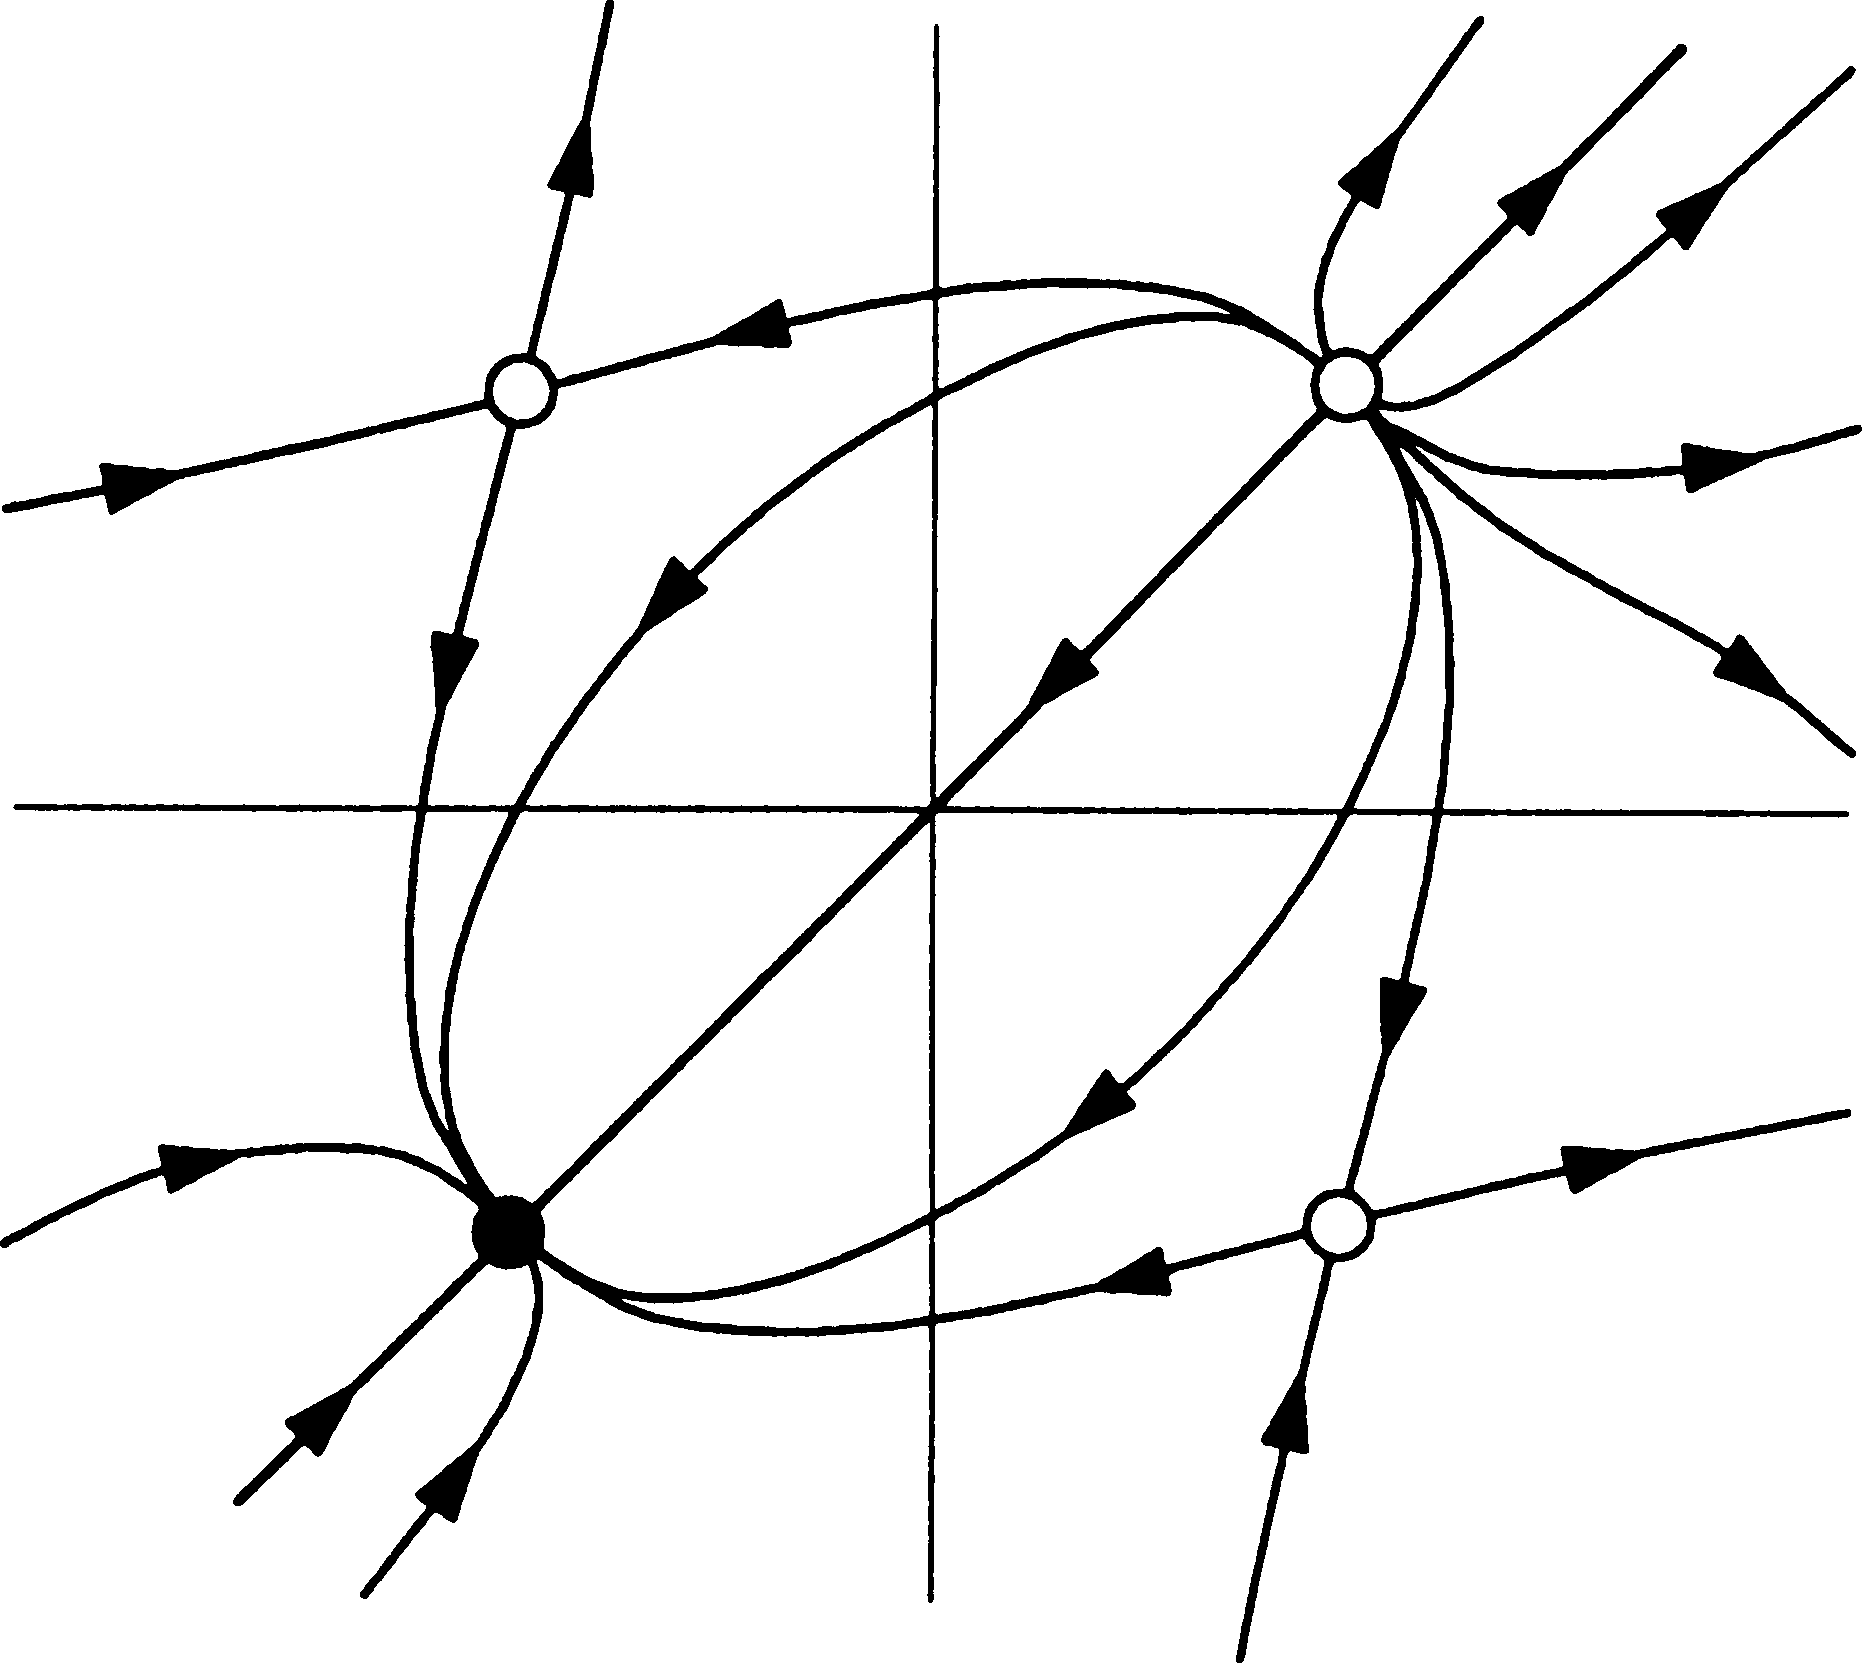
\includegraphics[width=0.82\textwidth]{images/Figures/figur-026.png}
\caption{Tersinir fakat korunumlu olmayan sistemin faz portresi.}
\label{fig:6-6-7}
\end{figure}
\end{justify}

\newpage
\section{Sarkaç}

\begin{justify}
Okulda incelediğiniz ilk doğrusal olmayan sistem muhtemelen sarkaçtı. Ancak temel derslerde sarkacın asıl doğrusal olmayan yapısı genellikle küçük açı yaklaşımı $\sin\theta\approx\theta$ ile geçiştirilir. Bu bölümde faz düzlemi yöntemleri kullanılarak sarkaç, büyük açı rejimi de dâhil olmak üzere incelenir.

Sönüm ve dış zorlama yokken sarkacın hareketi
\begin{equation}
\frac{d^2\theta}{dt^2}+\frac{g}{L}\sin\theta=0
\end{equation}
ile verilir. Burada $\theta$ aşağı düşey doğrultudan ölçülen açı, $g$ yerçekimi ivmesi ve $L$ sarkacın uzunluğudur (Şekil~\ref{fig:6-7-1}).

\begin{figure}[H]
\centering
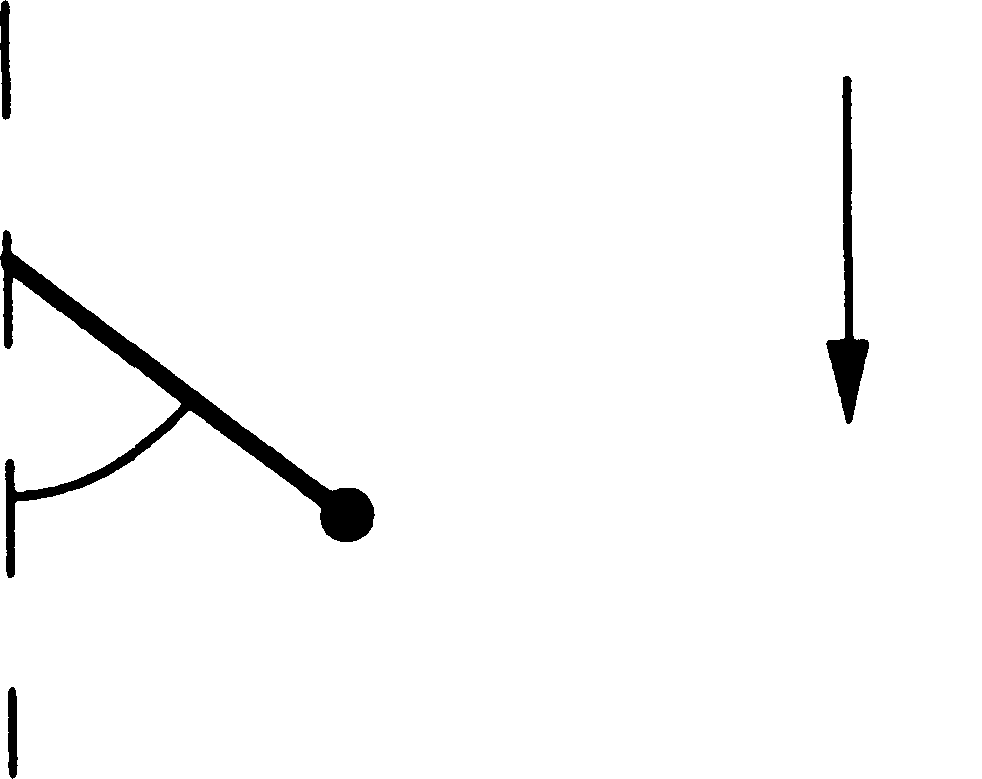
\includegraphics[width=0.82\textwidth]{images/Figures/figur-027.png}
\caption{Sarkacın geometrisi ve açı tanımı.}
\label{fig:6-7-1}
\end{figure}

Boyutsuzlaştırma için $\omega=\sqrt{g/L}$ ve $\tau=\omega t$ tanımlanır. Böylece denklem
\begin{equation}
\ddot{\theta}+\sin\theta=0
\end{equation}
hâline gelir; burada nokta $\tau$'ya göre türevi gösterir. Faz düzlemindeki karşılık gelen sistem
\begin{align}
\dot{\theta} &= v,\\
\dot{v} &= -\sin\theta
\end{align}
şeklindedir. Burada $v$ boyutsuz açısal hızdır.

Sabit noktalar $(\theta^{*},v^{*})=(k\pi,0)$ noktalarıdır; burada $k$ herhangi bir tam sayıdır. $2\pi$ kadar farklı olan açılar fiziksel olarak aynı olduğundan, $(0,0)$ ve $(\pi,0)$ noktalarına odaklanmak yeterlidir.

$(0,0)$ noktasında Jacobian
\begin{equation}
A=\begin{pmatrix}0&1\\-1&0\end{pmatrix}
\end{equation}
olur. Bu nedenle orijin doğrusal bir merkezdir. Aslında orijin doğrusal olmayan bir merkezdir. Bunun iki nedeni vardır: Sistem tersinirdir; $\tau\mapsto -\tau$, $v\mapsto -v$ dönüşümü altında denklemler değişmez. Ayrıca sistem korunumludur. Denklem $\dot{\theta}$ ile çarpılıp integre edilirse
\begin{equation}
\frac{1}{2}\dot{\theta}^{2}-\cos\theta=\text{sabit}
\end{equation}
bulunur. Enerji fonksiyonu
\begin{equation}
E(\theta,v)=\frac{1}{2}v^2-\cos\theta
\end{equation}
şeklindedir. Bu fonksiyonun $(0,0)$ noktasında yerel minimumu vardır; dolayısıyla orijin doğrusal olmayan bir merkezdir.

Şimdi sarkacı ters konumda, yani $(\pi,0)$ noktasında düşünelim. Bu noktadaki Jacobian
\begin{equation}
A=\begin{pmatrix}0&1\\1&0\end{pmatrix}
\end{equation}
olur. Karakteristik denklem $\lambda^2-1=0$ olduğundan $\lambda_1=-1$, $\lambda_2=1$ bulunur. Bu nokta bir eyer noktasıdır. Karşılık gelen özvektörler $(-1,1)$ ve $(1,1)$ doğrultularıdır.

Sabit noktalar yakınındaki faz portresi Şekil~\ref{fig:6-7-2}'de, enerji konturlarının eklenmesiyle elde edilen faz portresi ise Şekil~\ref{fig:6-7-3}'te gösterilecektir.

\begin{figure}[H]
\centering
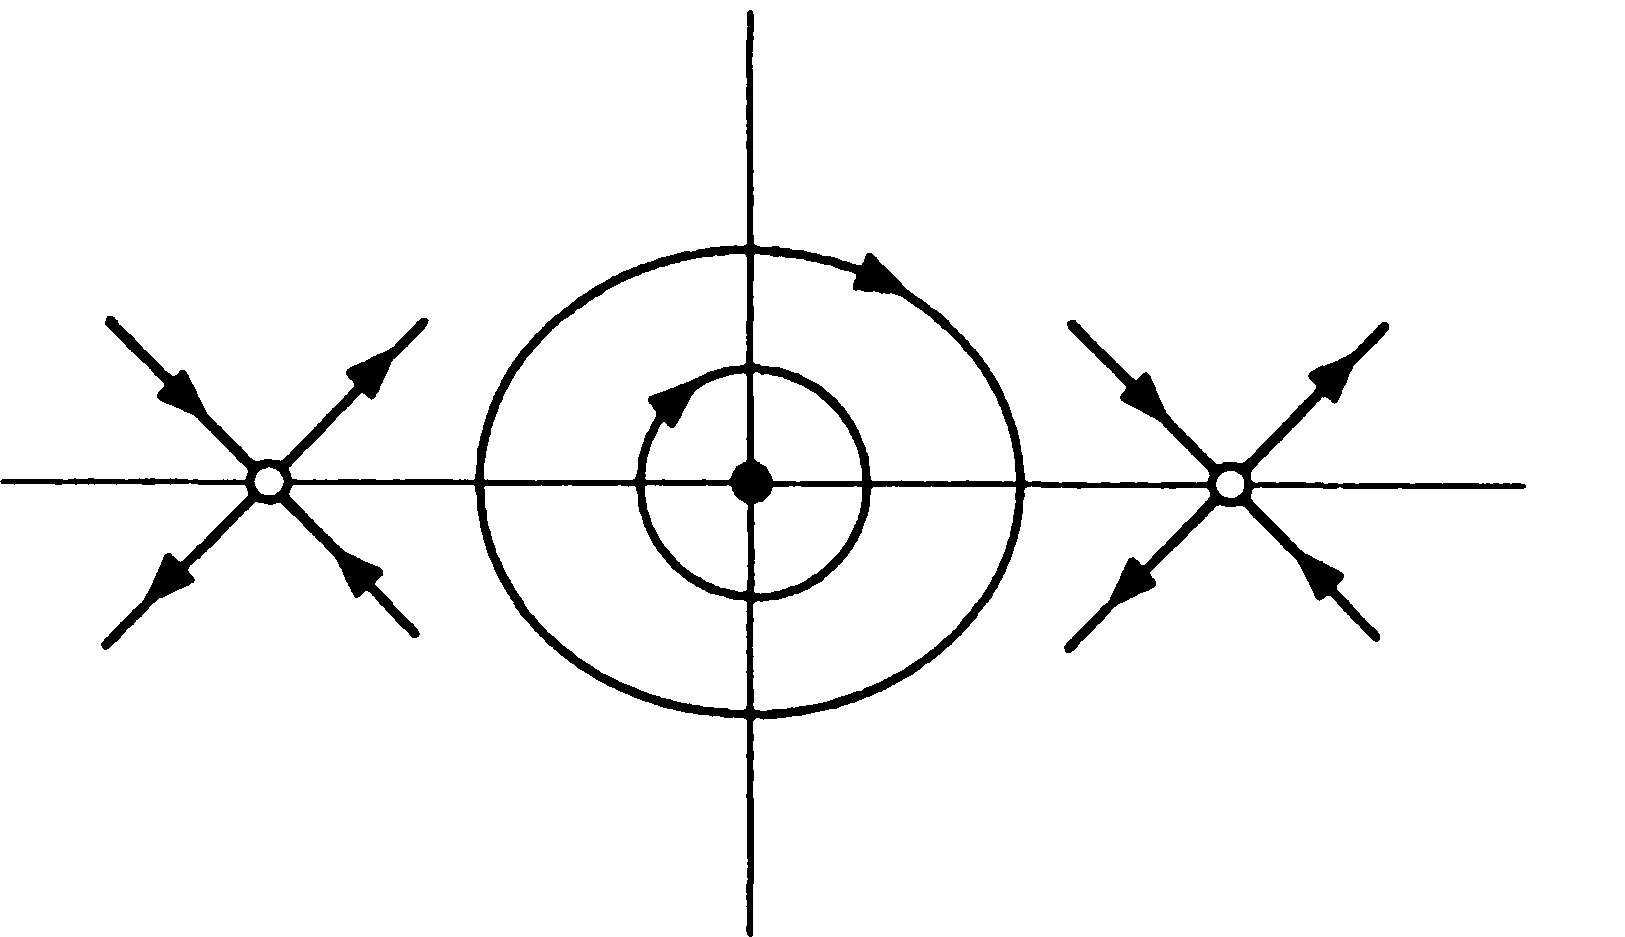
\includegraphics[width=0.82\textwidth]{images/Figures/figur-028.png}
\caption{Sarkaçta merkez ve eyer noktaları yakınındaki yerel faz portresi.}
\label{fig:6-7-2}
\end{figure}
\begin{figure}[H]
\centering
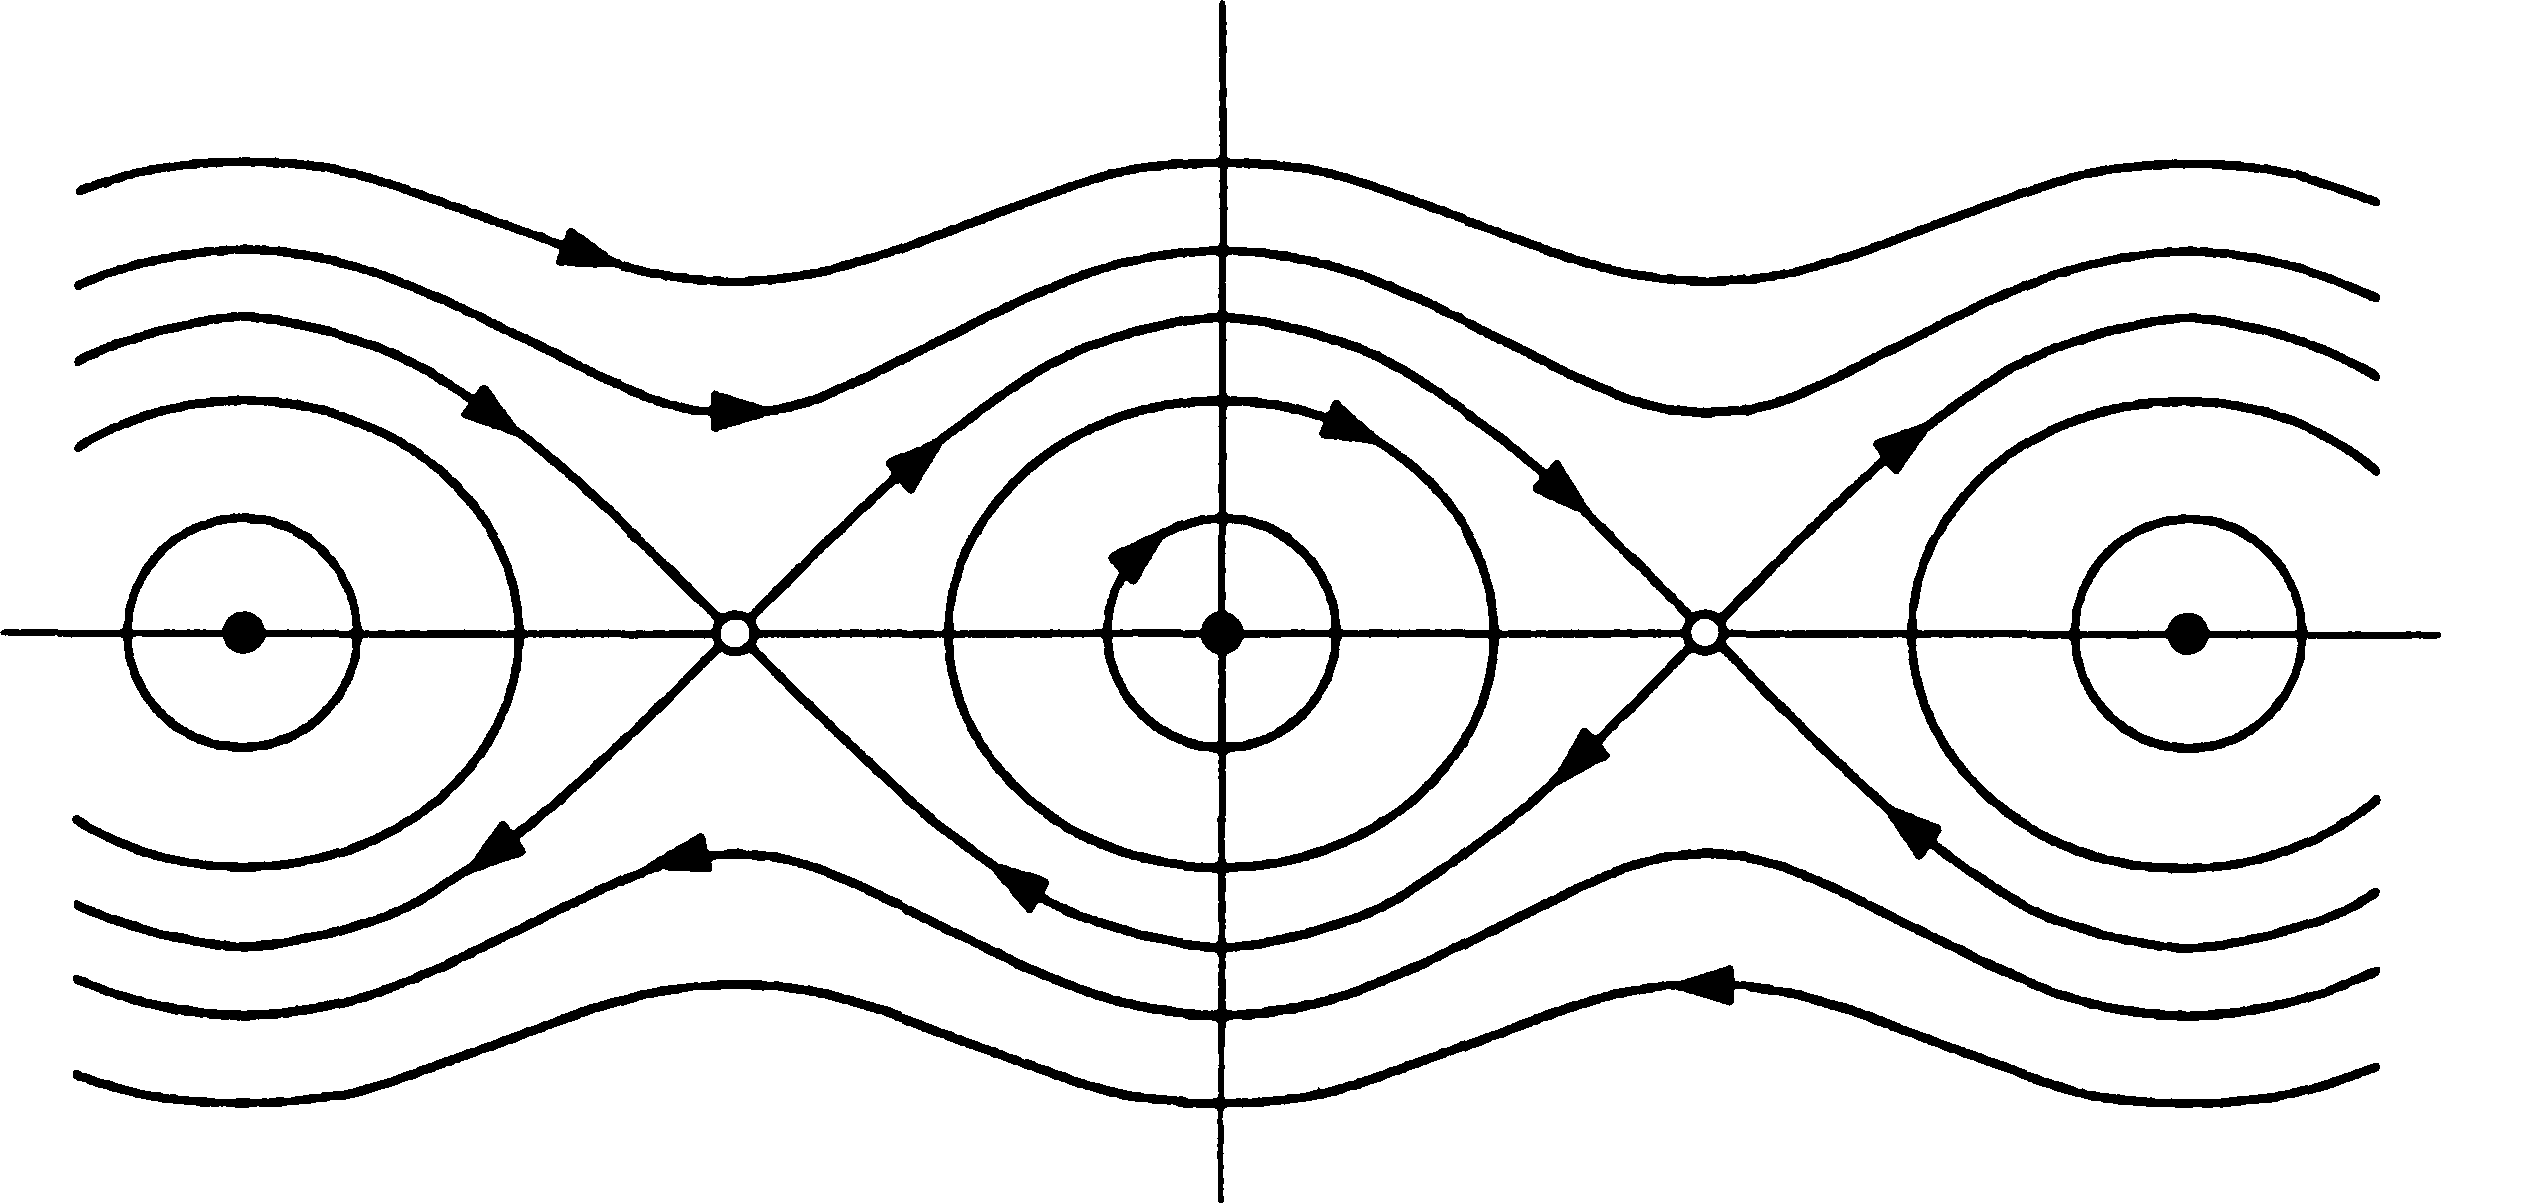
\includegraphics[width=0.82\textwidth]{images/Figures/figur-029.png}
\caption{Sönümsüz sarkaç için enerji konturları ve faz portresi.}
\label{fig:6-7-3}
\end{figure}

Fiziksel yorum şöyledir: Merkez, sarkacın aşağı doğru asılı ve dengede olduğu nötr kararlı duruma karşılık gelir. Bu en düşük enerji durumudur. Merkez çevresindeki küçük kapalı yörüngeler küçük salınımları temsil eder. $E=1$ kritik durumu, eyerleri birleştiren heteroklinik yörüngelere karşılık gelir. Bu yörüngeler ters çevrilmiş sarkaç durumunda hassas hareketleri temsil eder. $E>1$ olduğunda sarkaç tepeyi tekrar tekrar aşarak döner.
\end{justify}

\subsection*{Silindirik Faz Uzayı}
\addcontentsline{toc}{subsection}{Silindirik Faz Uzayı}

\begin{justify}
Sarkacın faz portresi, silindir yüzeyine sarıldığında daha aydınlatıcı olur (Şekil~\ref{fig:6-7-4}). Gerçekte sarkaç için doğal faz uzayı silindirdir; çünkü açısal hız $v$ gerçek bir sayı iken $\theta$ bir açıdır.

\begin{figure}[H]
\centering
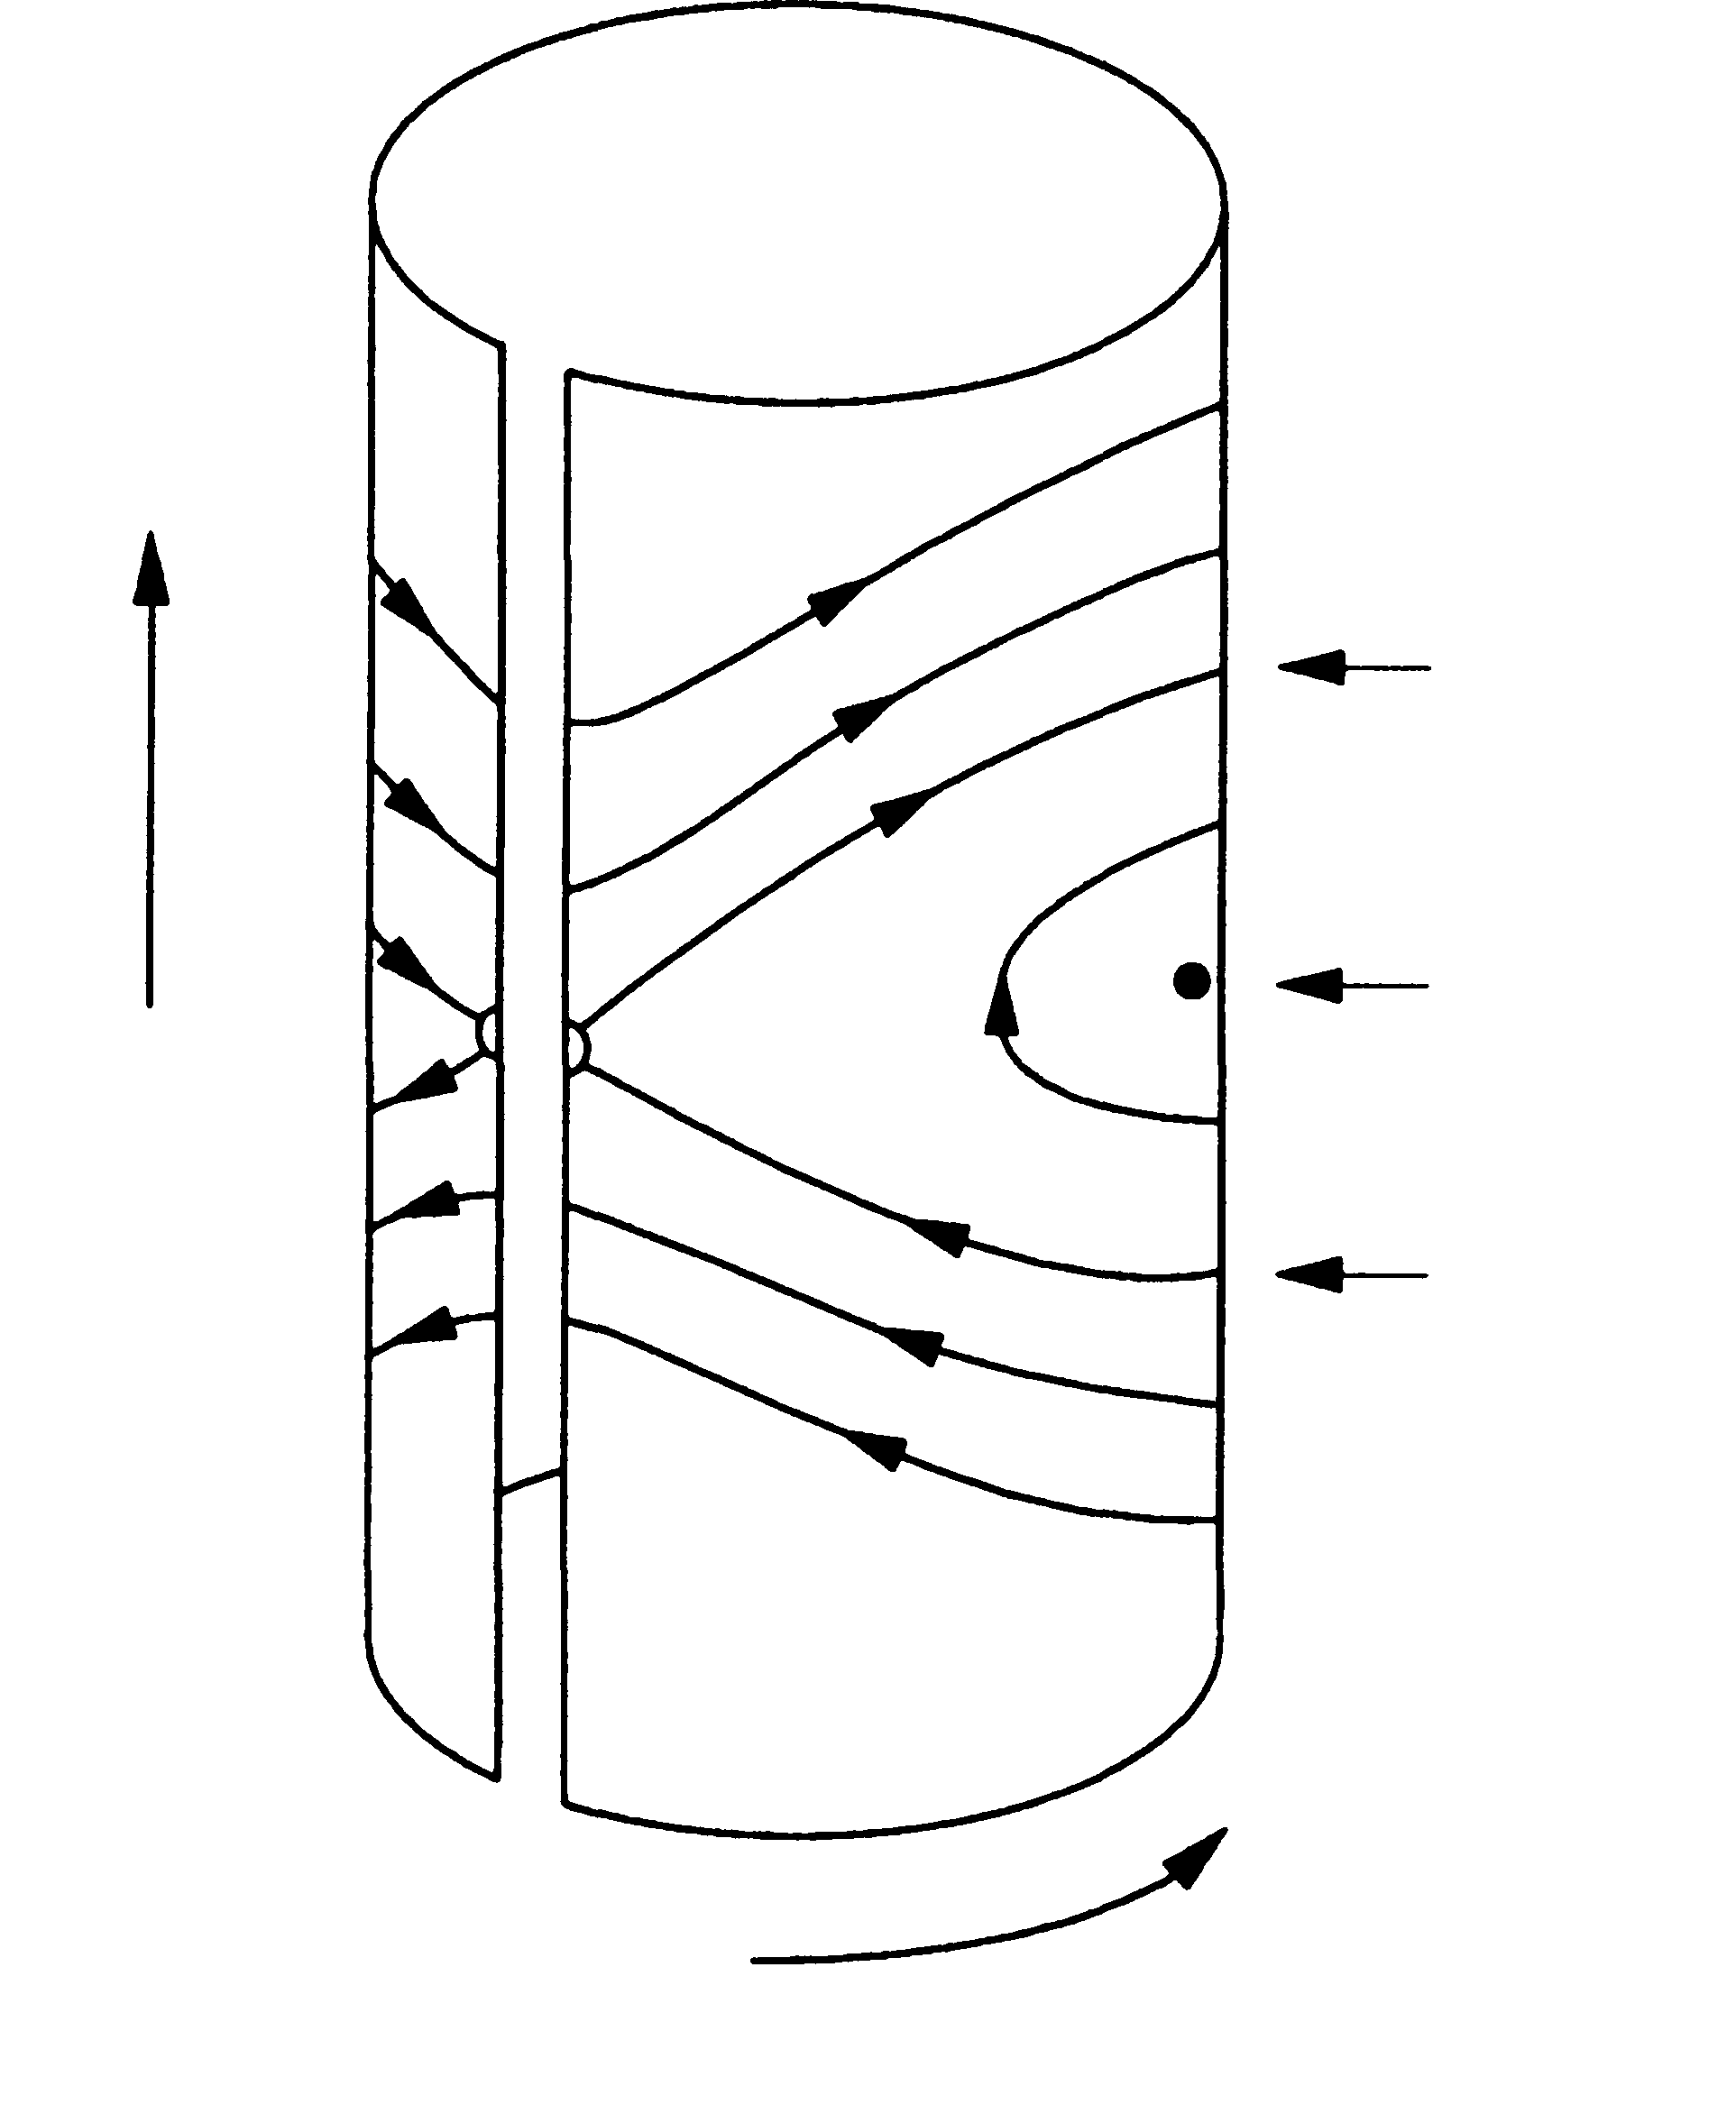
\includegraphics[width=0.82\textwidth]{images/Figures/figur-030.png}
\caption{Sarkacın silindirik faz uzayındaki faz portresi.}
\label{fig:6-7-4}
\end{figure}

Silindirik gösterimin birkaç avantajı vardır. $E>1$ için periyodik dönme hareketleri artık gerçekten periyodik görünür; bunlar silindiri çevreleyen kapalı yörüngelerdir. Ayrıca Şekil~\ref{fig:6-7-3}'teki eyer noktalarının fiziksel olarak aynı durumu, yani tepe konumunda duran ters sarkacı temsil ettiği açık hâle gelir. Düzlemde heteroklinik görünen yörüngeler silindir üzerinde homoklinik yörüngelere dönüşür.

Enerjiyi açısal hız yerine dikey eksende çizmek simetriyi daha açık gösterir. Bu durumda yörüngeler sabit yükseklikte kalırken silindir U biçimli bir tüpe bükülür (Şekil~\ref{fig:6-7-5}). Tüpün iki kolu sarkacın saat yönünde ya da saat yönünün tersinde dönmesini temsil eder. Düşük enerjilerde bu ayrım ortadan kalkar; sarkaç ileri geri salınır. Homoklinik yörüngeler $E=1$ seviyesinde, dönmeler ile salınımlar arasındaki sınırda bulunur.

\begin{figure}[H]
\centering
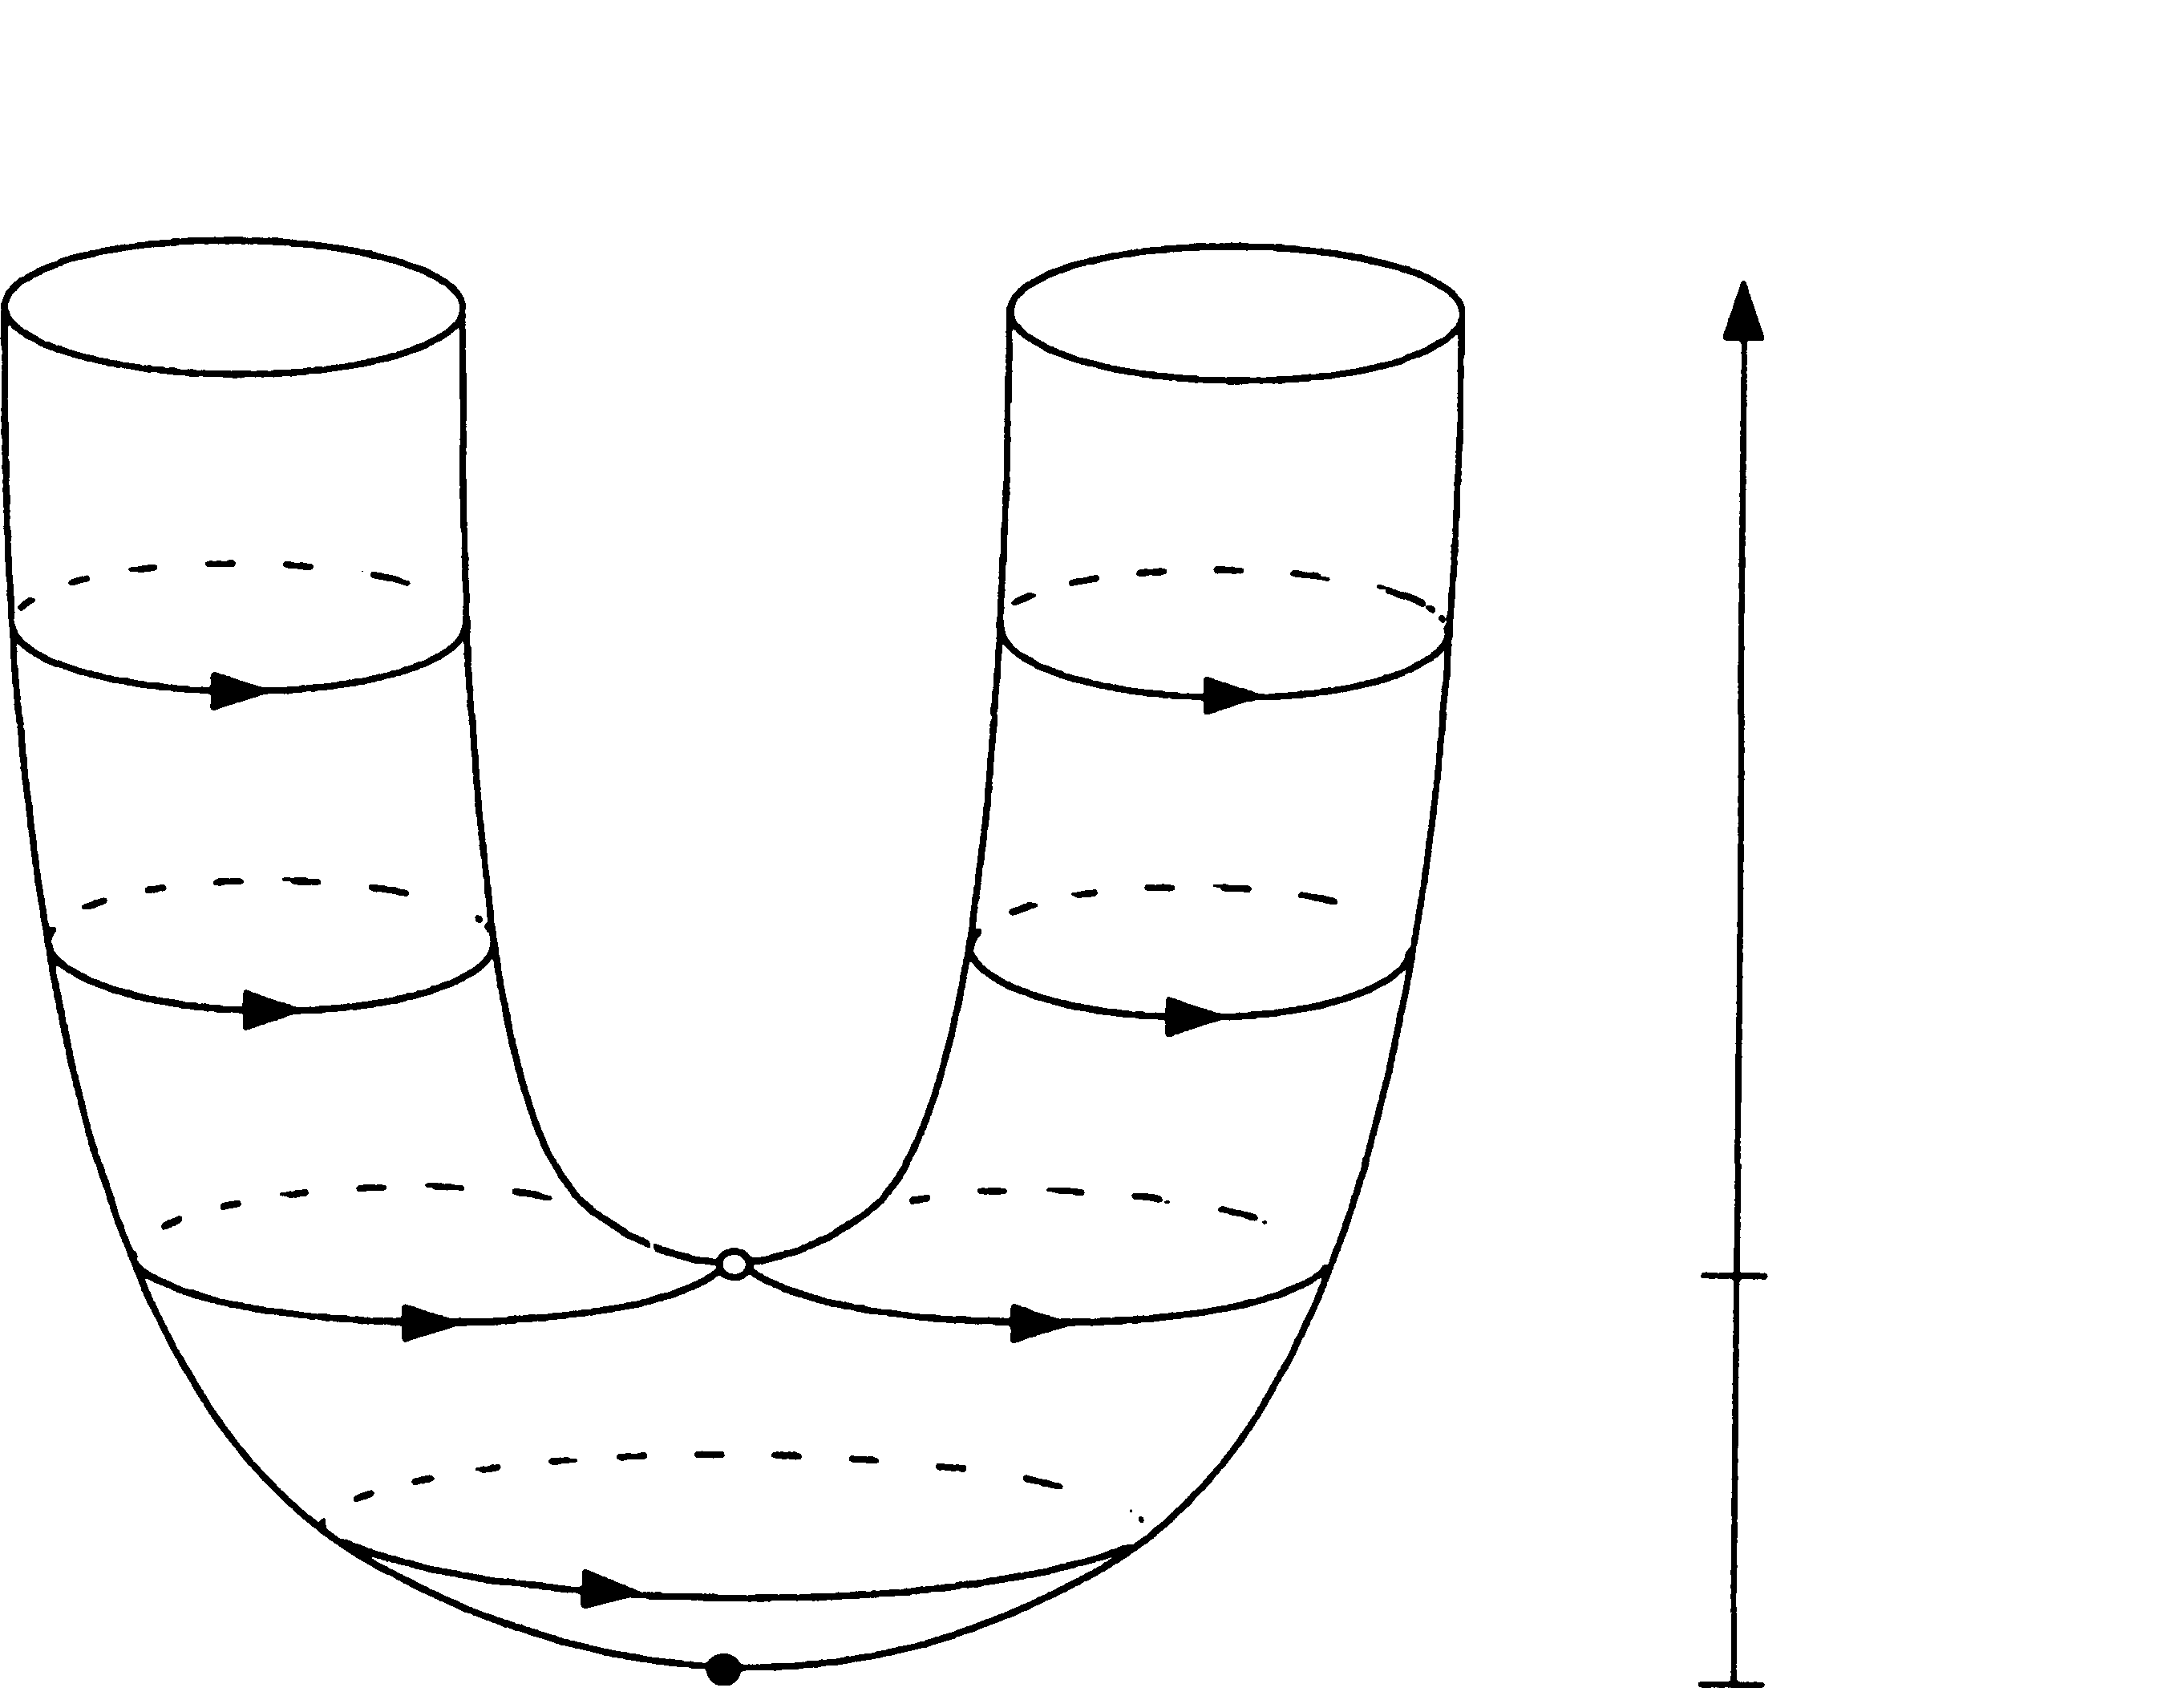
\includegraphics[width=0.82\textwidth]{images/Figures/figur-031.png}
\caption{Enerjinin dikey eksende çizildiği U-tüp gösterimi.}
\label{fig:6-7-5}
\end{figure}

İlk bakışta U-tüpün kollarından birindeki oklar ters çizilmiş gibi görünebilir. Ancak koordinat sistemine bakıldığında çizimin doğru olduğu anlaşılır (Şekil~\ref{fig:6-7-6}). Silindirin alt kısmı U-tüp oluşturacak biçimde büküldüğünde artan $\theta$ yönü tersine dönmüştür.

\begin{figure}[H]
\centering
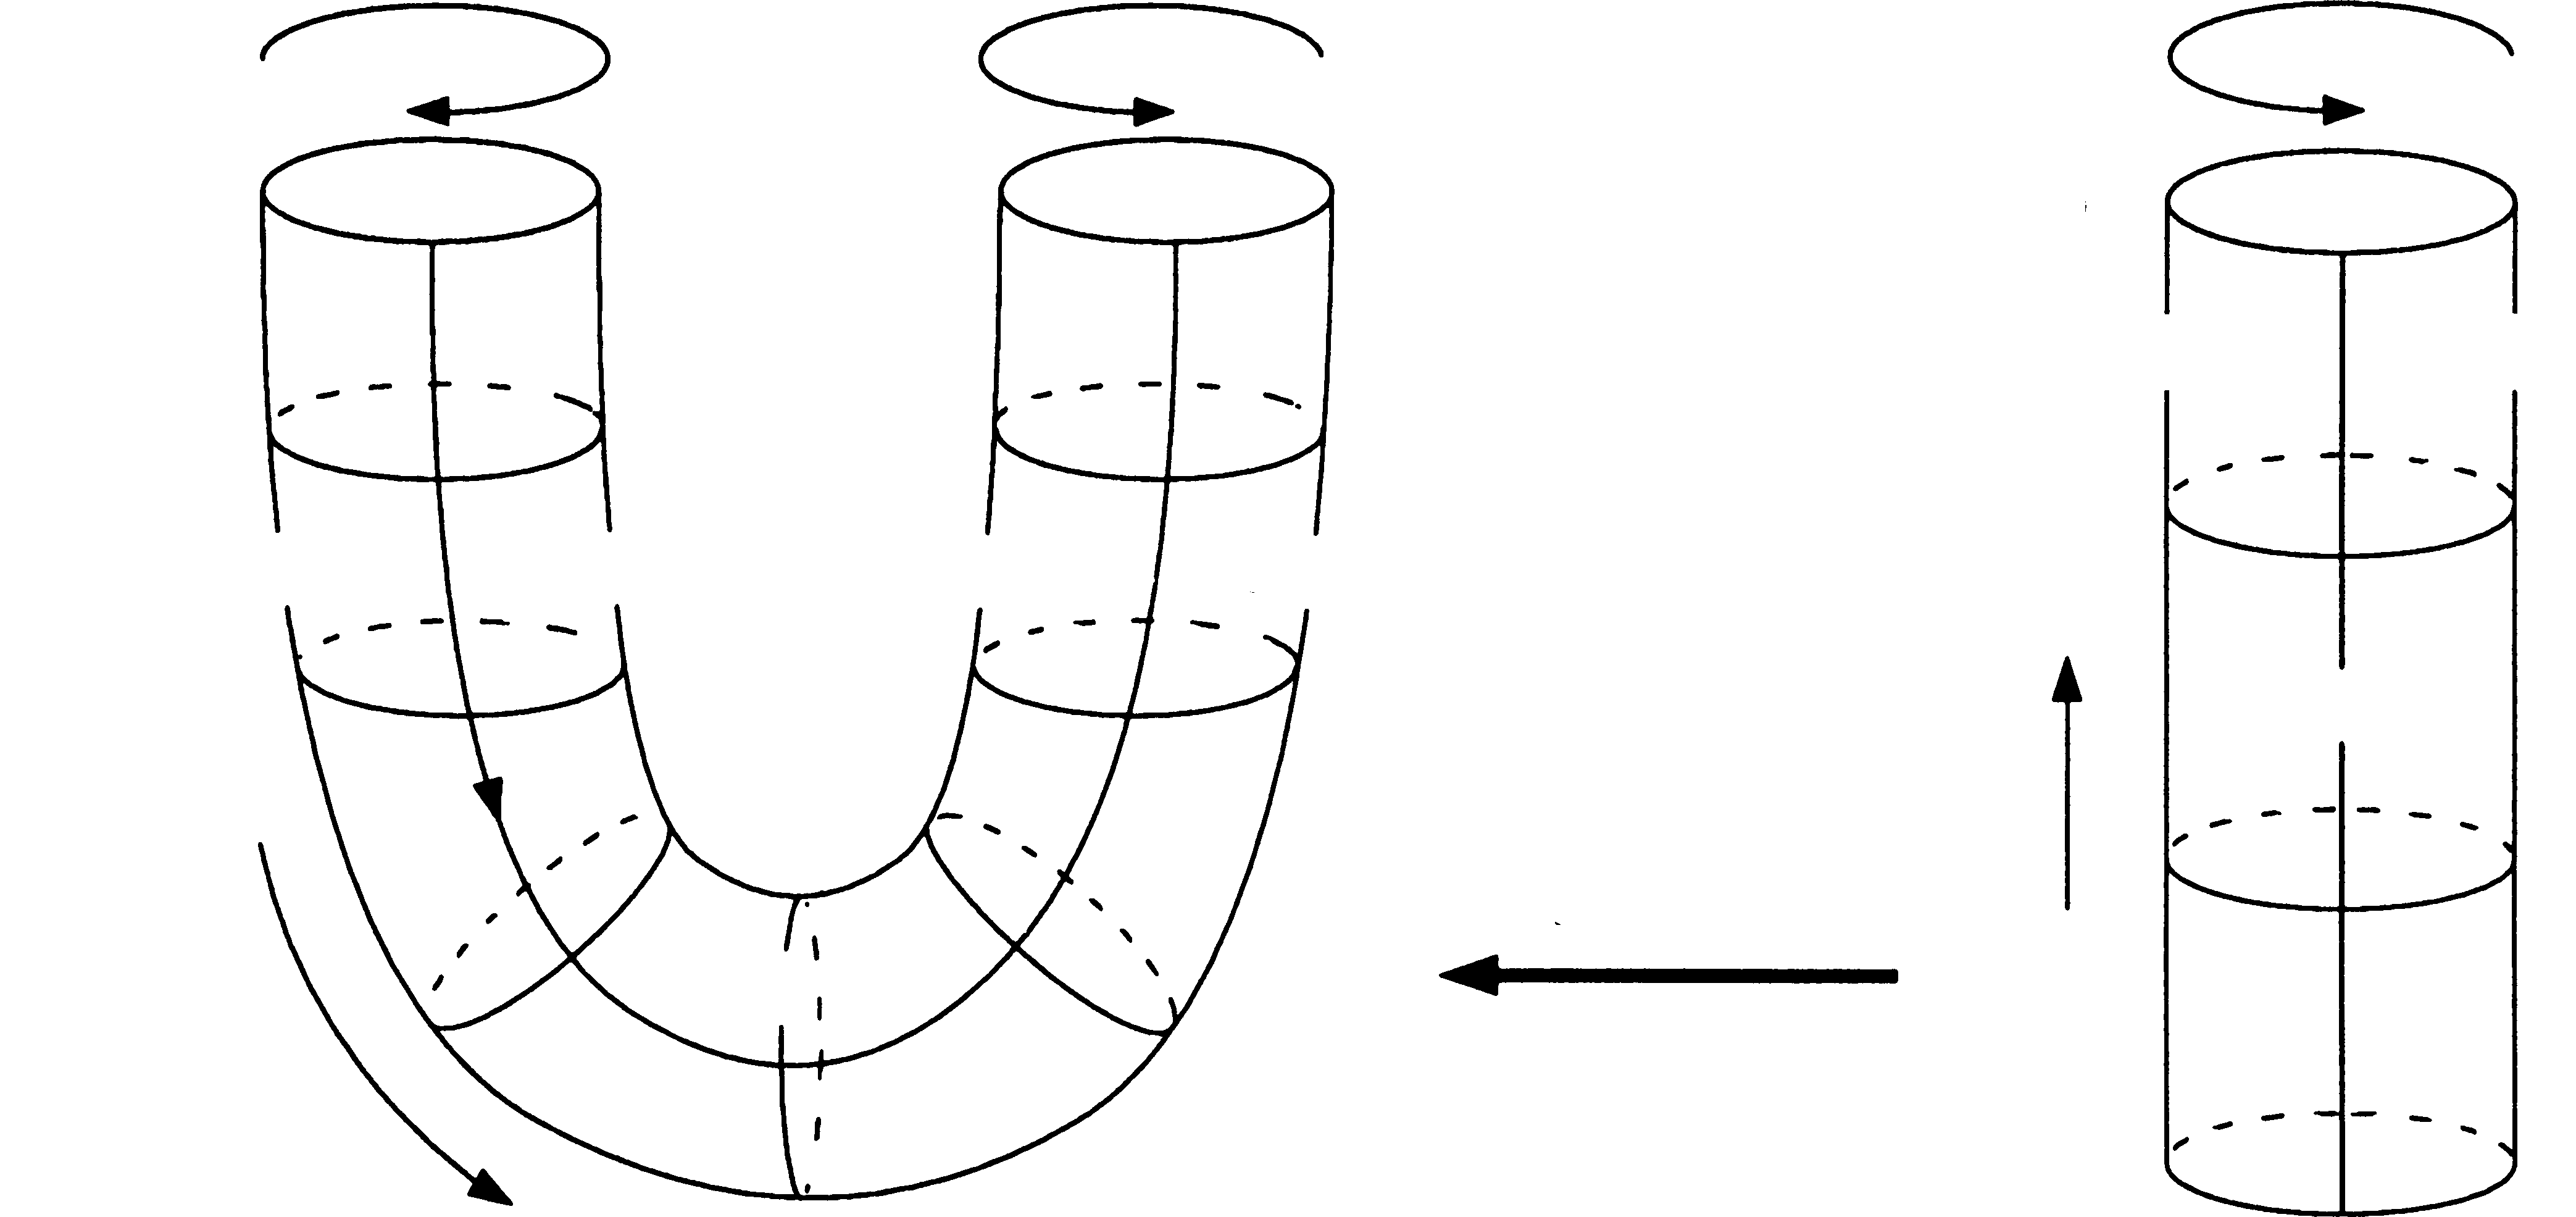
\includegraphics[width=0.82\textwidth]{images/Figures/figur-032.png}
\caption{Silindirik koordinat sisteminin U-tüp gösterimine bükülmesi.}
\label{fig:6-7-6}
\end{figure}
\end{justify}

\subsection*{Sönüm}
\addcontentsline{toc}{subsection}{Sönüm}

\begin{justify}
Şimdi faz düzlemine geri dönelim ve sarkaca küçük miktarda doğrusal sönüm ekleyelim. Denklem
\begin{equation}
\ddot{\theta}+b\dot{\theta}+\sin\theta=0
\end{equation}
olur; burada $b>0$ sönüm şiddetidir. Bu durumda merkezler kararlı spirallere dönüşürken eyerler eyer olarak kalır. Bilgisayar üretimli faz portresi Şekil~\ref{fig:6-7-7}'de gösterilecektir.

\begin{figure}[H]
\centering
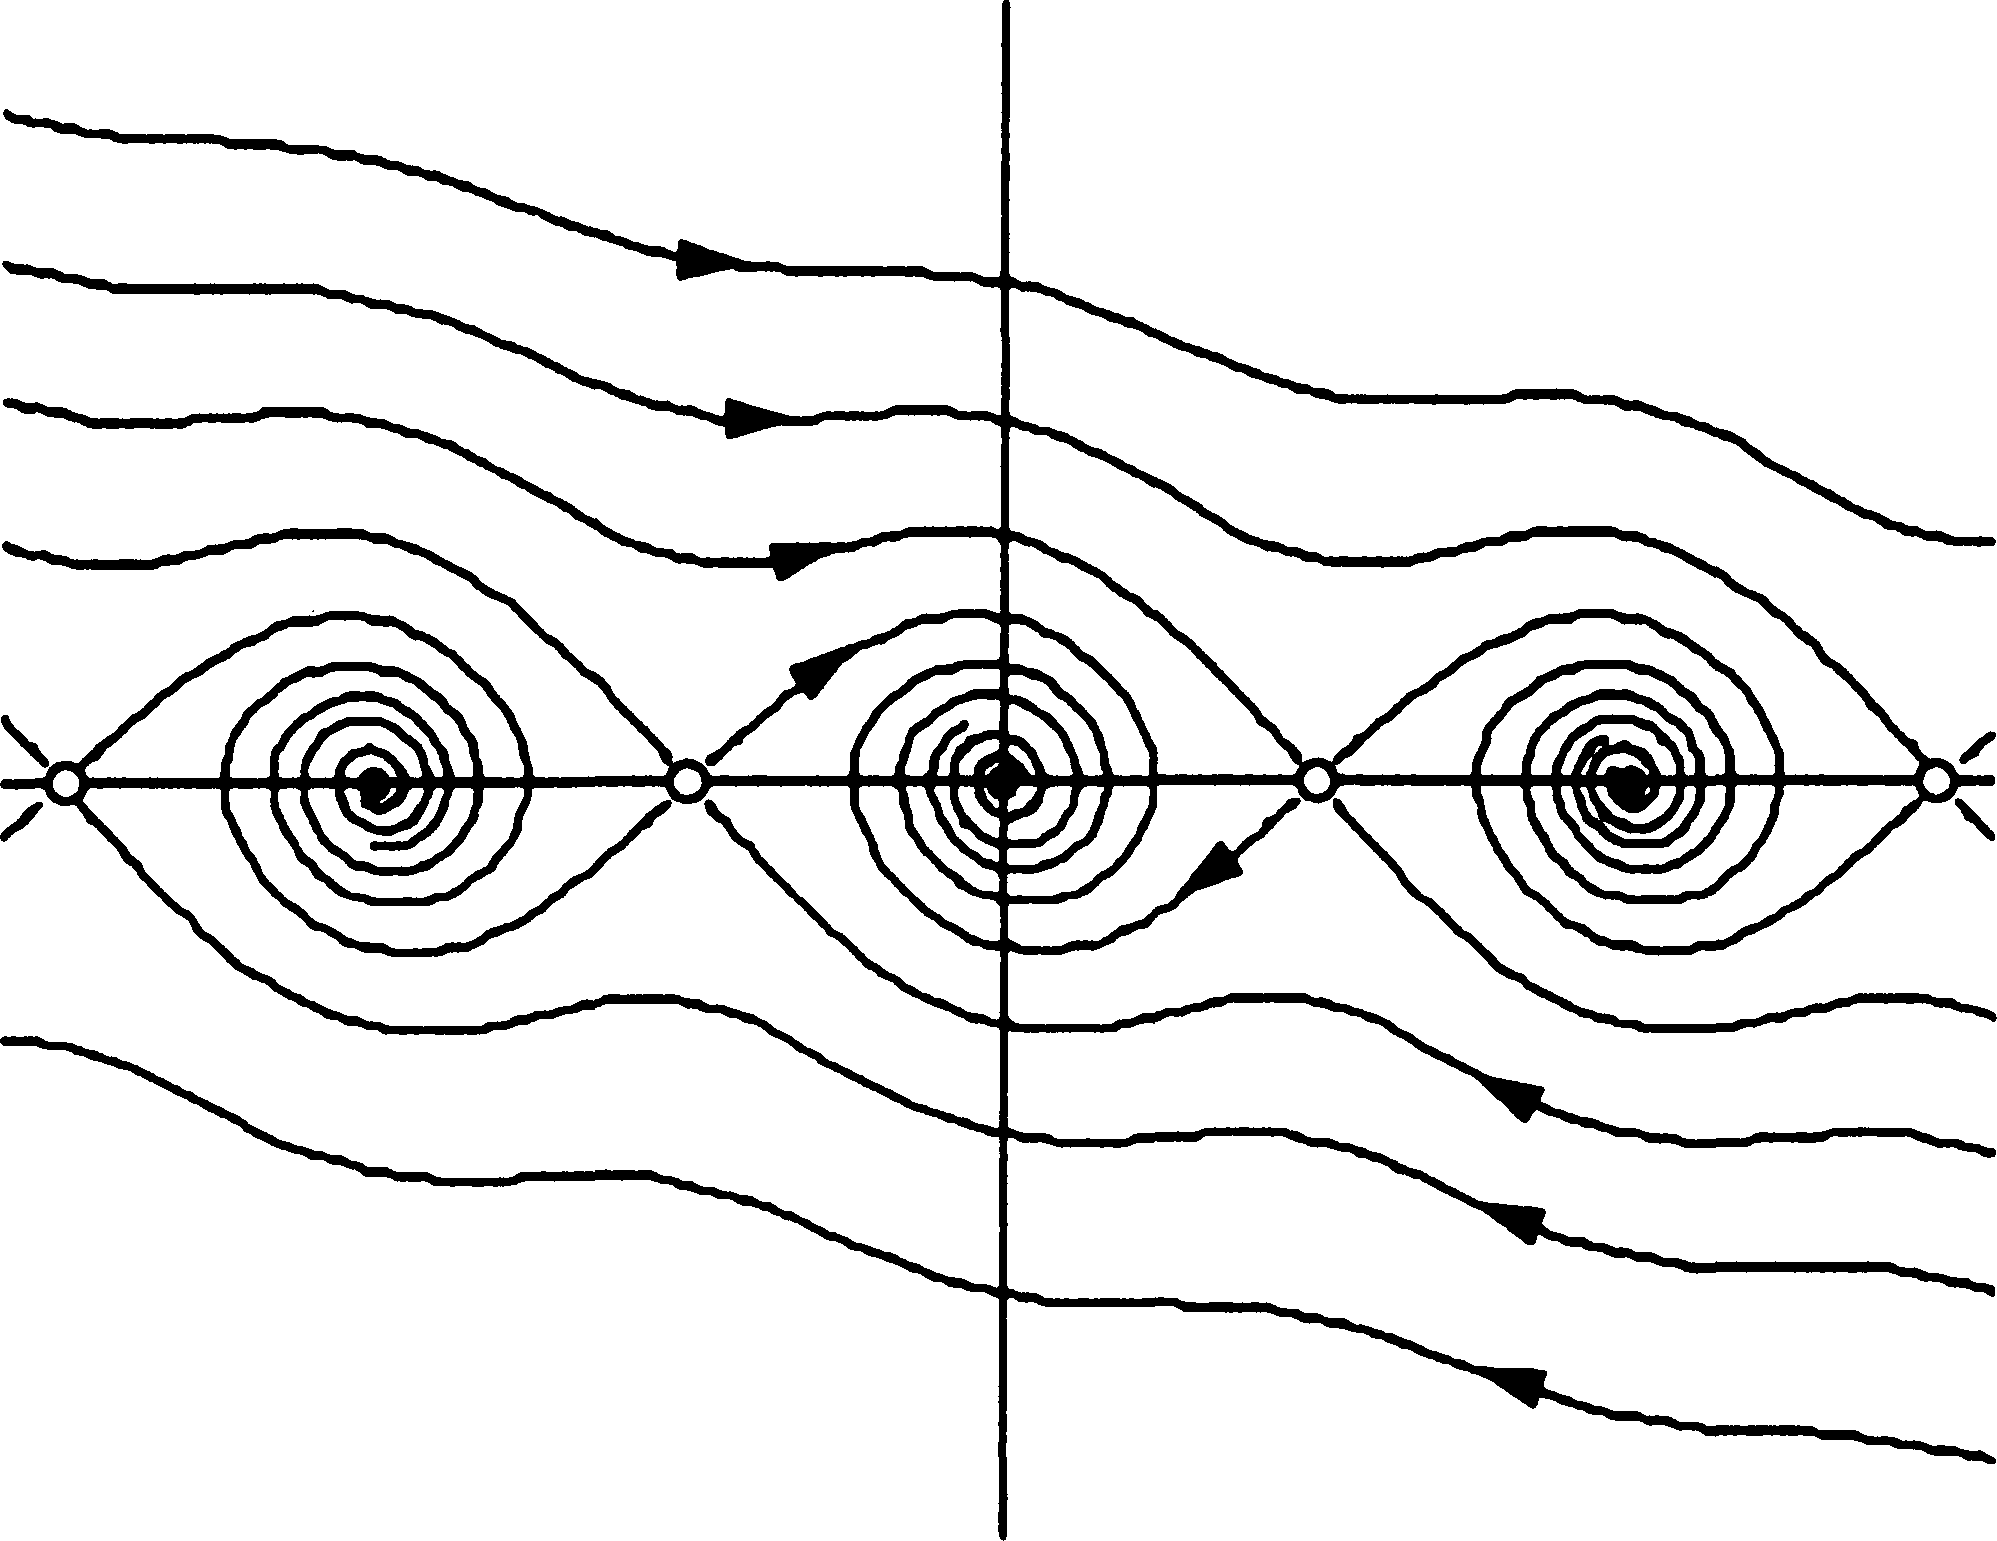
\includegraphics[width=0.82\textwidth]{images/Figures/figur-033.png}
\caption{Sönümlü sarkaç için faz portresi.}
\label{fig:6-7-7}
\end{figure}

U-tüp gösteriminde durum daha açıktır: sabit noktalar dışında tüm yörüngeler sürekli irtifa kaybeder (Şekil~\ref{fig:6-7-8}). Enerjinin yörünge boyunca değişimi
\begin{equation}
\frac{dE}{d\tau}
=\frac{d}{d\tau}\left(\frac{1}{2}\dot{\theta}^2-\cos\theta\right)
=\dot{\theta}(\ddot{\theta}+\sin\theta)
=-b\dot{\theta}^{2}\le 0
\end{equation}
şeklindedir. Dolayısıyla sabit noktalar dışında enerji yörüngeler boyunca monoton olarak azalır.

\begin{figure}[H]
\centering
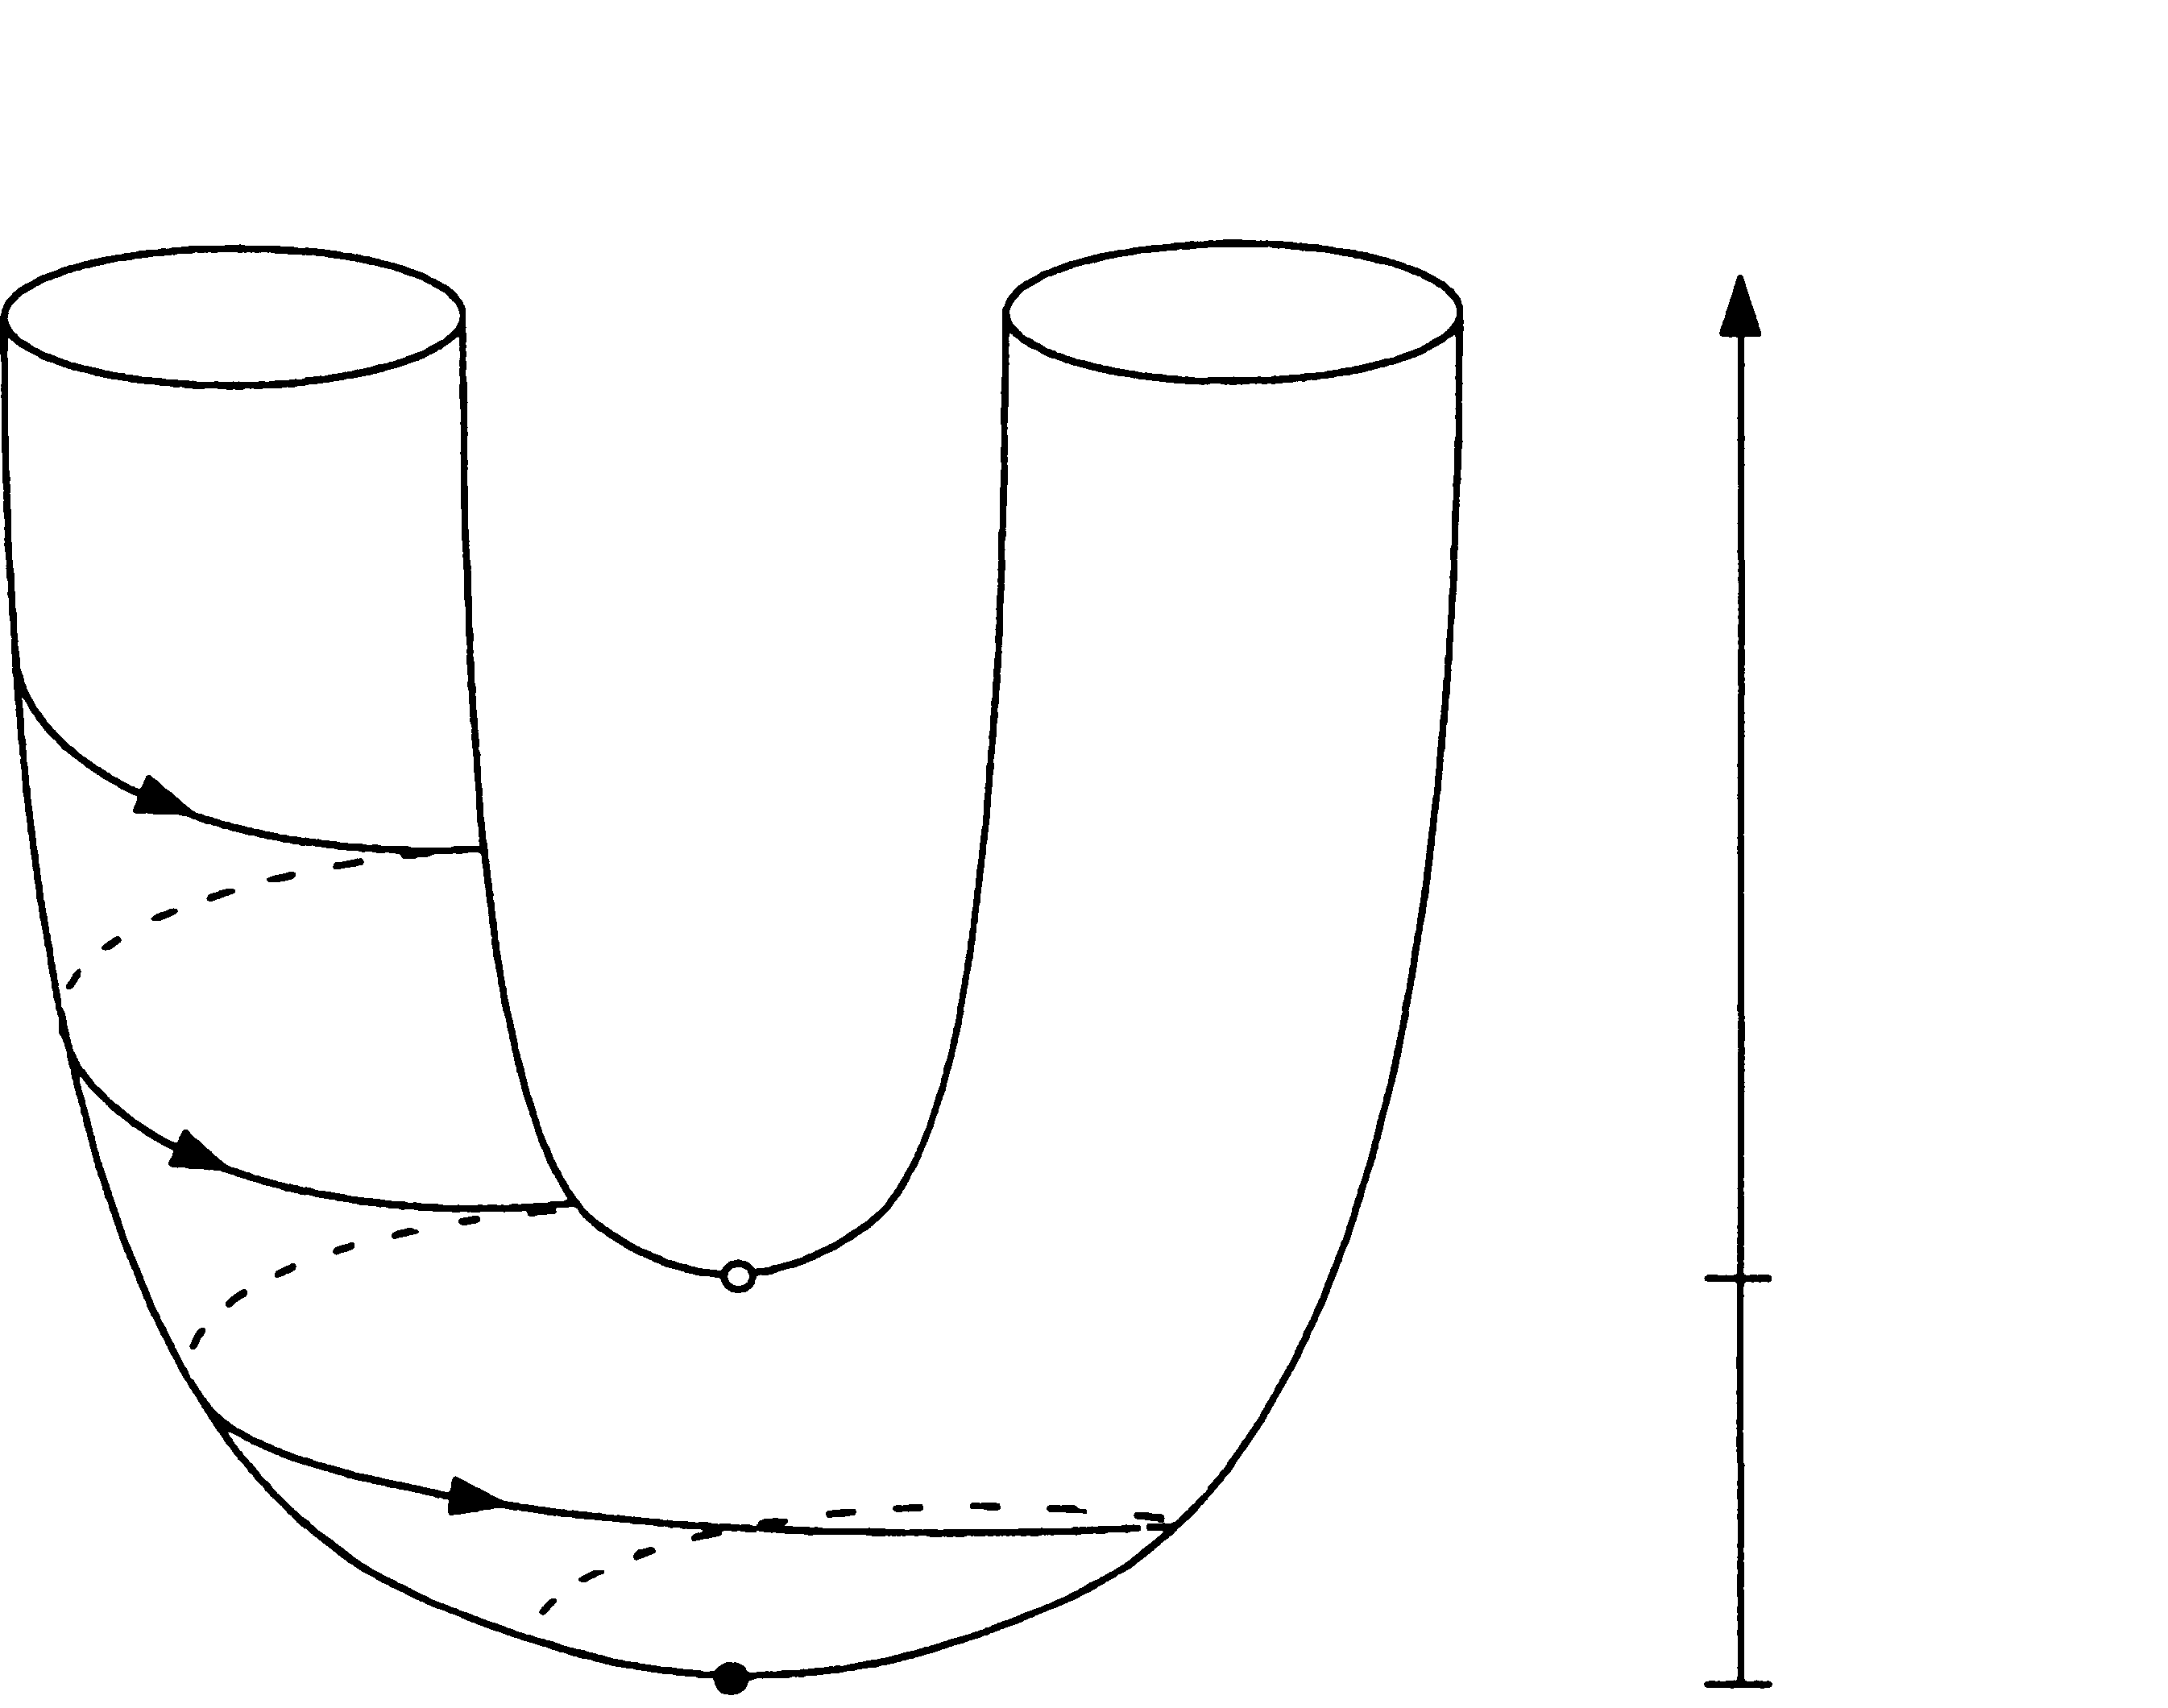
\includegraphics[width=0.82\textwidth]{images/Figures/figur-034.png}
\caption{Sönümlü sarkacın U-tüp enerji gösterimi.}
\label{fig:6-7-8}
\end{figure}

Şekil~\ref{fig:6-7-8}'deki yörüngenin fiziksel yorumu şudur: sarkaç başlangıçta saat yönünde dönmektedir. Enerji kaybettikçe tepeyi aşması zorlaşır. Karşılık gelen yörünge U-tüpün kolundan aşağı doğru spirallenir; $E<1$ olduğunda sarkaç artık dönemeyecek kadar az enerjiye sahiptir ve taban etrafında küçük salınımlara yerleşir. Sonunda hareket sönümlenir ve sarkaç kararlı dengesinde durur.

Bu örnek, yalnızca faz portresi resimleriyle sarkacın dinamiğinin temel özelliklerinin çıkarılabileceğini gösterir. Aynı sonuçları analitik formüllerle elde etmek çok daha zor ve yorumlamak daha karmaşık olurdu.
\end{justify}

\newpage
\section{İndeks Teorisi}

\begin{justify}
Faz düzleminde kapalı eğriler yalnızca yörüngeleri değil, aynı zamanda bu eğrilerin içinde kalan sabit noktalar hakkında da bilgi taşır. İndeks teorisi bu fikri nicelleştirir. Amaç, bir kapalı eğri boyunca vektör alanının kaç kez döndüğünü sayarak eğrinin içinde hangi tür sabit noktaların bulunabileceğini anlamaktır.

Önce sabit nokta içermeyen, basit kapalı bir eğri $C$ seçelim. Eğri üzerinde saat yönünün tersine bir tur atarken vektör alanı $\mathbf{f}(x,y)=(\dot{x},\dot{y})$ her noktada sıfırdan farklı bir vektör verir. Bu vektörün yatay eksenle yaptığı açı $\phi$ olsun. Eğri boyunca bir tam tur sonunda $\phi$ açısının toplam değişimi $2\pi$'nin tam katı olmak zorundadır. Bu tam sayıya $C$ eğrisinin indeksi denir:
\begin{equation}
I_C=\frac{1}{2\pi}\Delta\phi.
\end{equation}

Başka bir deyişle indeks, vektör alanı oklarının eğri boyunca kaç tam dönüş yaptığını ölçer. Eğer oklar toplamda bir kez saat yönünün tersine dönerse $I_C=1$, bir kez saat yönünde dönerse $I_C=-1$ olur. Hiç net dönüş yoksa indeks sıfırdır.

\begin{figure}[H]
\centering
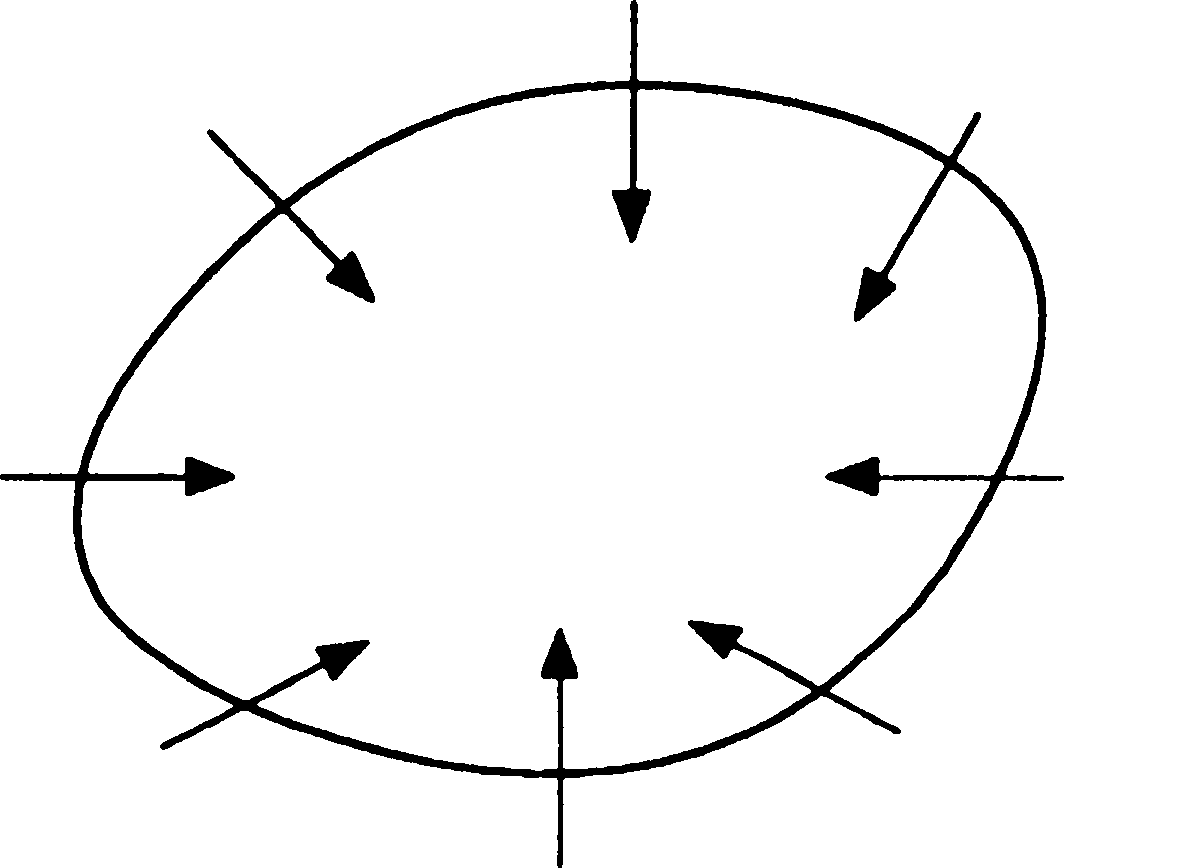
\includegraphics[width=0.82\textwidth]{images/Figures/figur-035.png}
\caption{Kapalı bir eğri boyunca vektör alanı yönünün dönmesi ve indeksin tanımı.}
\label{fig:6-8-1}
\end{figure}

İndeksin en önemli özelliği topolojik kararlılığıdır. Eğri, üzerinden sabit nokta geçirmeyecek biçimde sürekli olarak deforme edilirse indeks değişmez. Çünkü vektör alanı eğri üzerinde hiçbir zaman sıfır olmadığı sürece $\phi$ açısındaki toplam dönüş ancak sürekli değişebilir; fakat indeks bir tam sayı olduğundan sıçrama yapmadan değişemez.
\end{justify}

\subsection*{Sabit Noktaların İndeksi}
\addcontentsline{toc}{subsection}{Sabit Noktaların İndeksi}

\begin{justify}
Yalıtılmış bir sabit noktanın indeksi, bu noktayı çevreleyen küçük bir kapalı eğrinin indeksi olarak tanımlanır. Eğri yeterince küçük seçildiğinde başka sabit nokta içermez; bu nedenle elde edilen sayı yalnızca sabit noktanın yerel yapısına bağlıdır.

Düğüm, spiral ve merkez tipindeki sabit noktaların indeksi $+1$'dir. Bu durum sezgisel olarak açıktır: Bu noktaların çevresinde dolaşırken vektör alanı da bir tam tur döner. Buna karşılık eyer noktasının indeksi $-1$'dir. Eyerin kararlı ve kararsız doğrultuları vektör alanının yönünü öyle değiştirir ki toplam dönüş saat yönünde bir tur olur.

\begin{figure}[H]
\centering
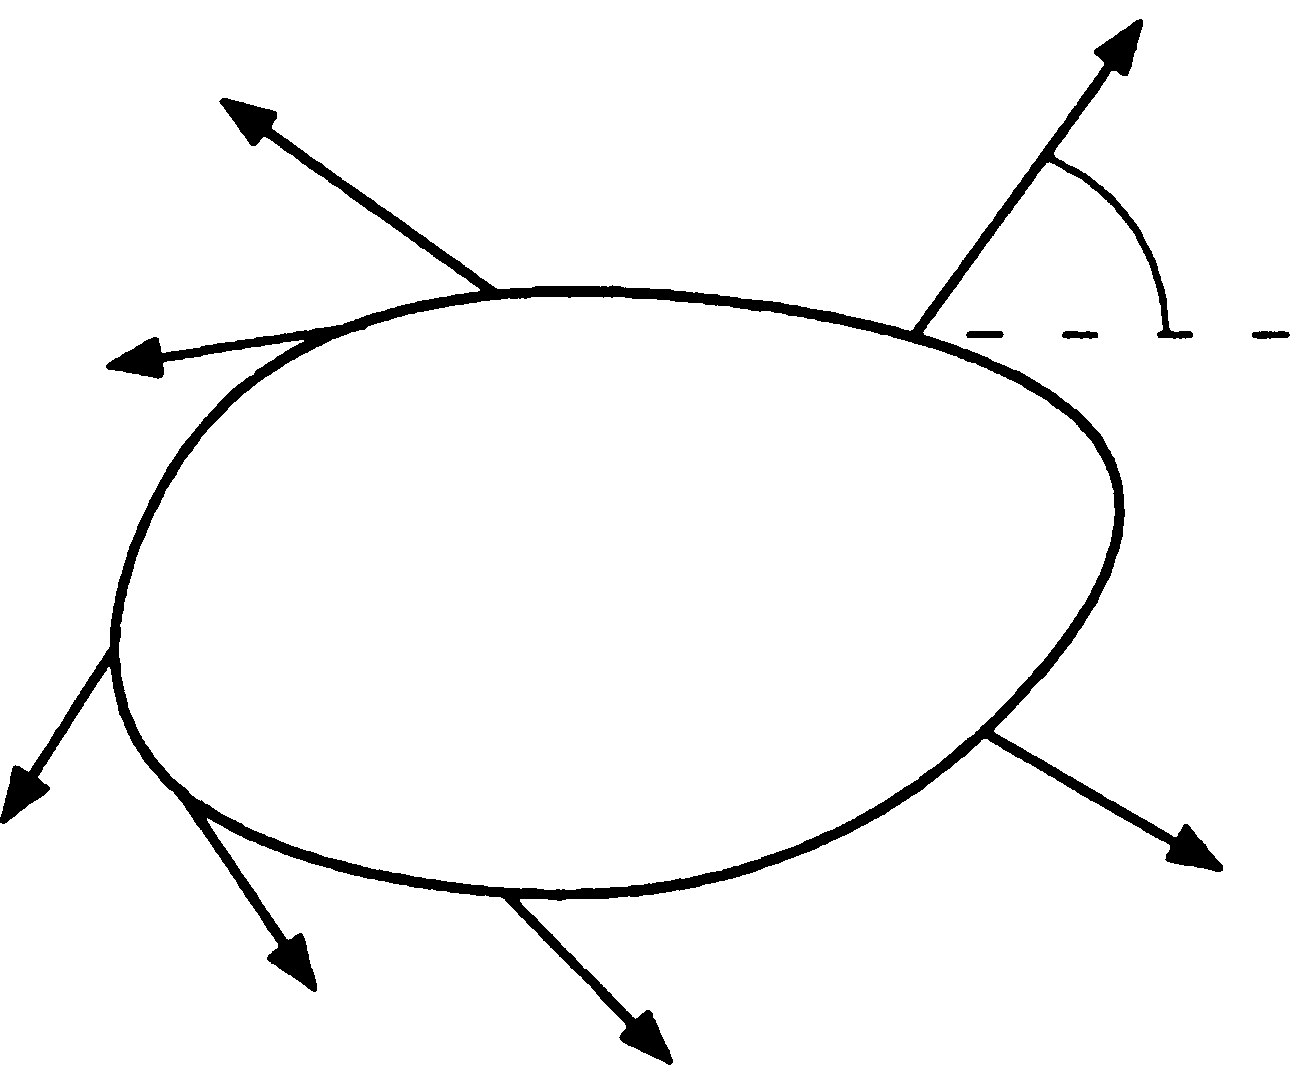
\includegraphics[width=0.82\textwidth]{images/Figures/figur-036.png}
\caption{Düğüm, spiral, merkez ve eyer noktalarının indeksleri.}
\label{fig:6-8-2}
\end{figure}

Bu sonuçlar doğrusal sistemler üzerinden de görülebilir. Lineerleştirme matrisi tekil değilse, sabit nokta hiperboliktir ve yerel faz portresi doğrusal sistemle aynı topolojik tipe sahiptir. Bu durumda
\begin{equation}
\text{indeks}=\operatorname{sgn}(\det A)
\end{equation}
şeklinde yorumlanabilir. $\det A>0$ olduğunda düğüm, spiral ya da merkez benzeri davranış ortaya çıkar ve indeks $+1$ olur. $\det A<0$ olduğunda sabit nokta eyer noktasıdır ve indeks $-1$ olur.
\end{justify}

\subsection*{İndekslerin Toplanması}
\addcontentsline{toc}{subsection}{İndekslerin Toplanması}

\begin{justify}
Bir kapalı eğri $C$ içinde sonlu sayıda yalıtılmış sabit nokta bulunsun ve eğrinin üzerinde sabit nokta olmasın. Bu durumda $C$ eğrisinin indeksi, içerdiği sabit noktaların indekslerinin toplamına eşittir:
\begin{equation}
I_C=\sum_{k} I_k.
\end{equation}

Bu kural faz portrelerini hızlı biçimde denetlemek için çok yararlıdır. Örneğin kapalı bir eğrinin indeksi $+1$ ise, eğrinin içinde yalnızca bir merkez bulunabilir; ya da bir eyer ve iki düğüm gibi toplam indeksi yine $+1$ yapan başka kombinasyonlar olabilir. Fakat tek başına bir eyer, indeksi $-1$ olduğundan böyle bir eğrinin içinde bulunamaz.

\begin{figure}[H]
\centering
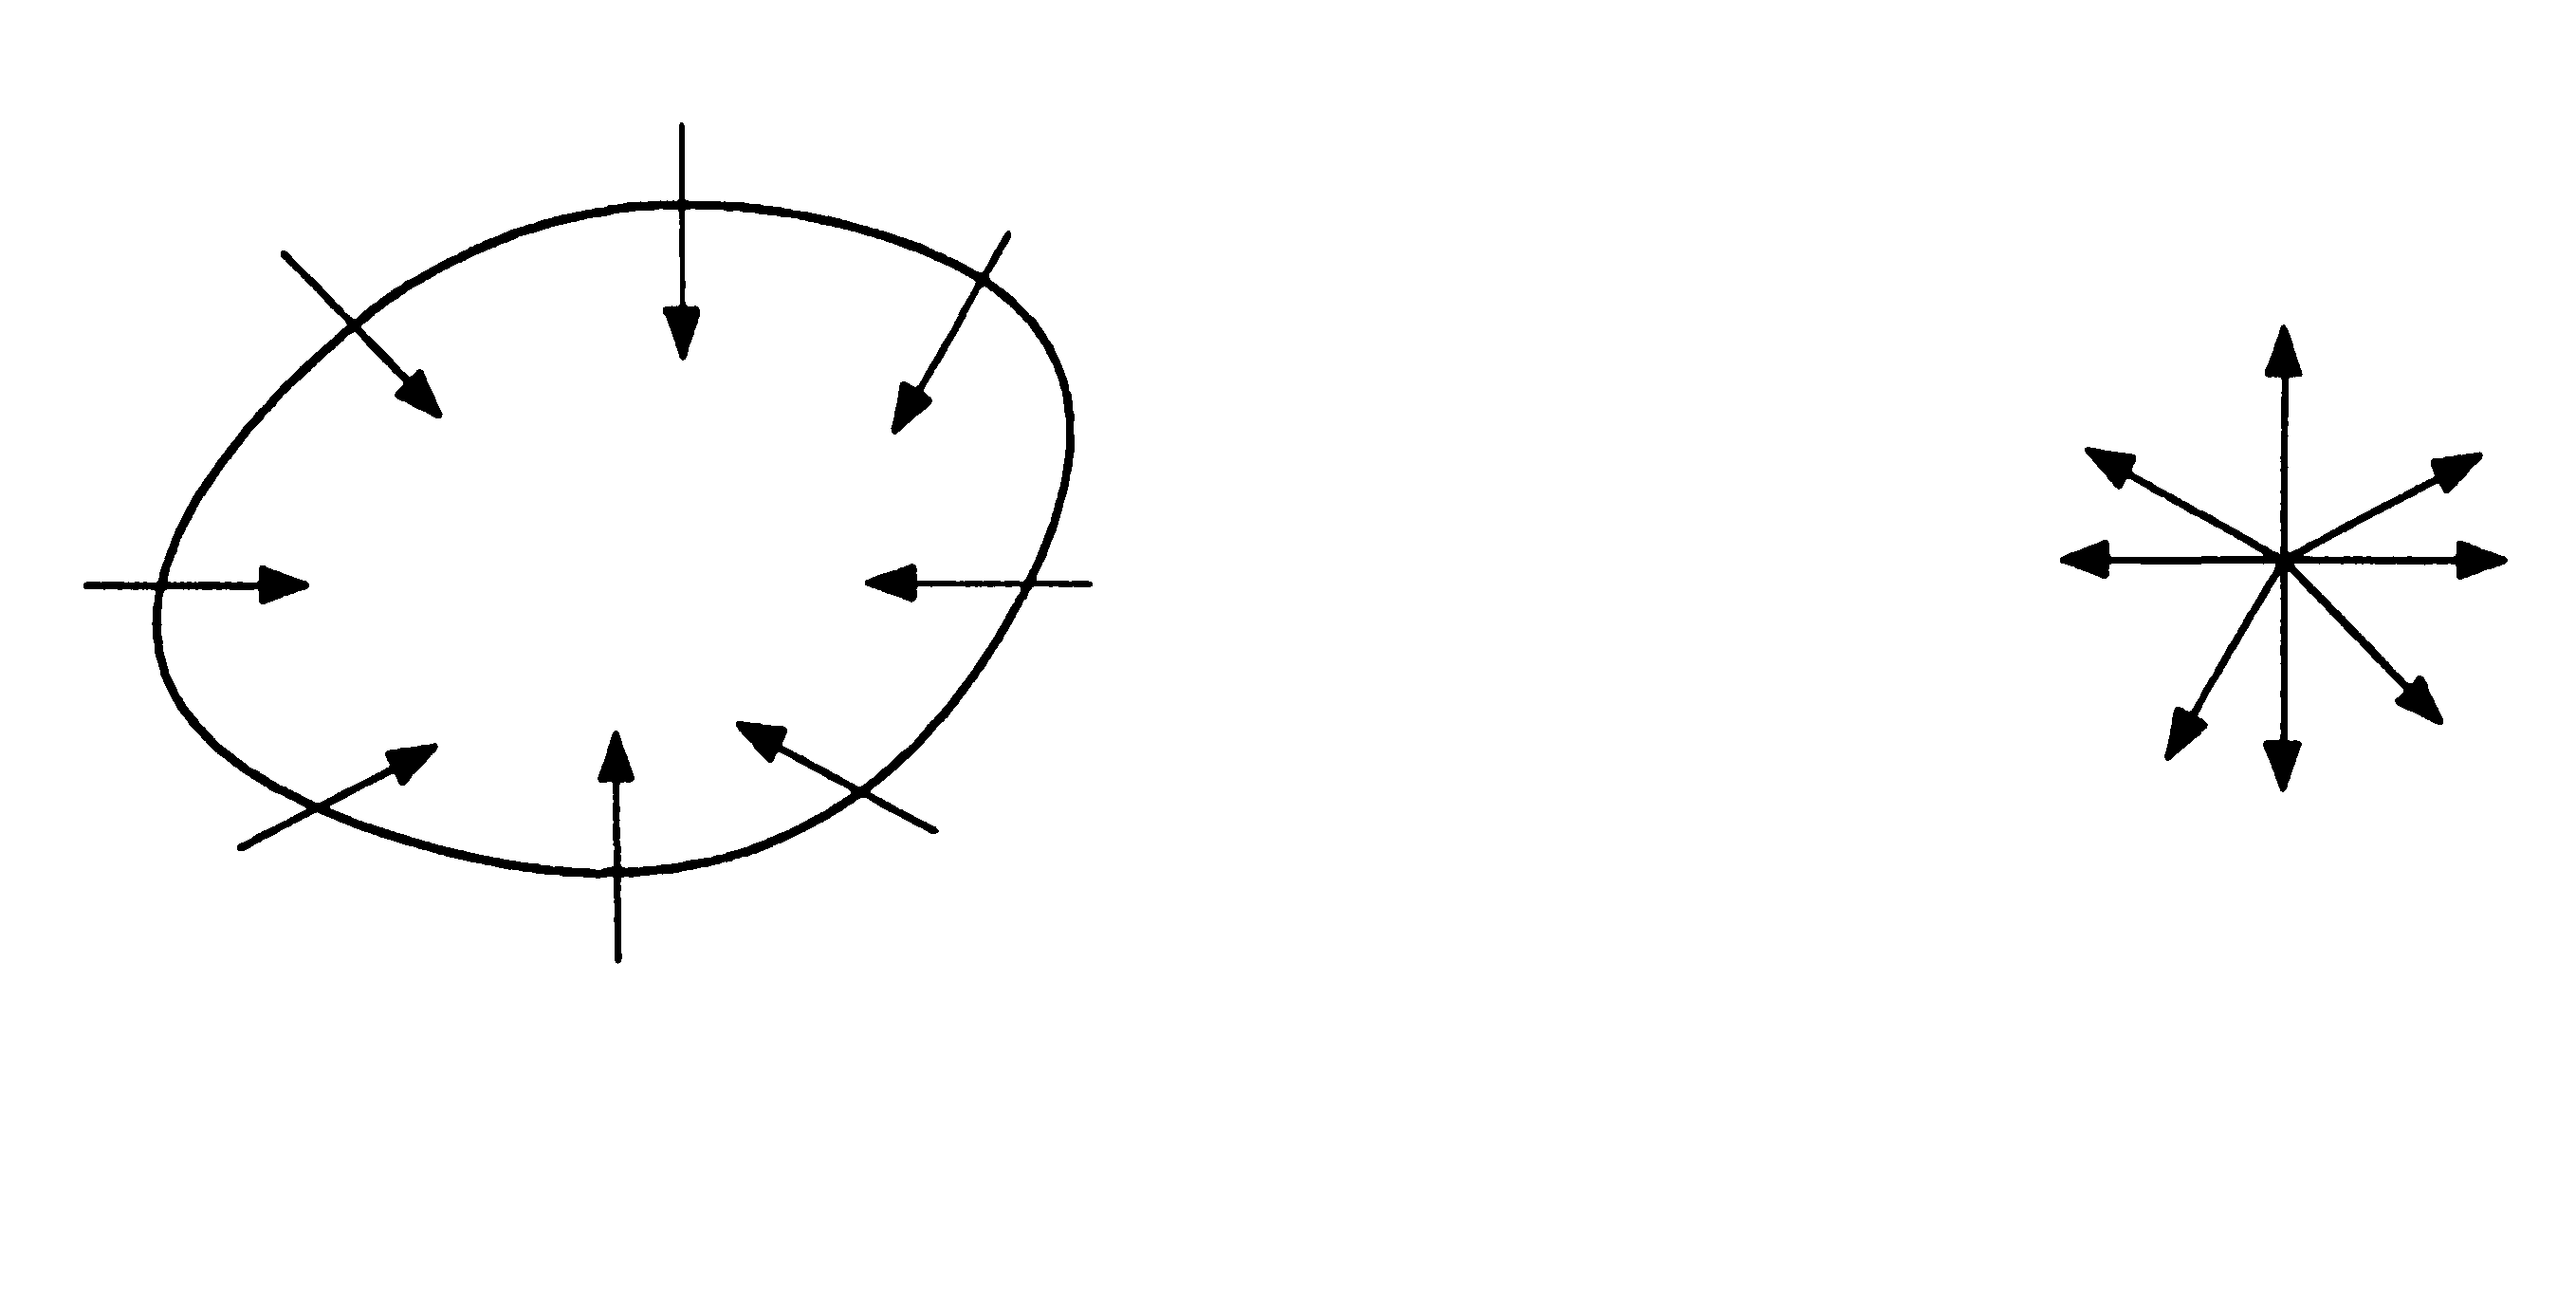
\includegraphics[width=0.82\textwidth]{images/Figures/figur-037.png}
\caption{Bir kapalı eğrinin indeksinin içerdiği sabit noktaların indeksleri toplamına eşit olması.}
\label{fig:6-8-3}
\end{figure}

Özel olarak, kapalı bir yörüngeyi ele alalım. Yörüngenin kendisi boyunca vektör alanı eğriye teğettir ve hareket yönünü gösterir. Kapalı yörünge bir tur tamamladığında teğet vektörü de bir tam tur döner. Dolayısıyla kapalı yörüngenin indeksi
\begin{equation}
I_C=1
\end{equation}
olur. Buradan önemli bir sonuç çıkar: Her kapalı yörüngenin içinde toplam indeksi $+1$ olan en az bir sabit nokta bulunmalıdır.

\begin{figure}[H]
\centering
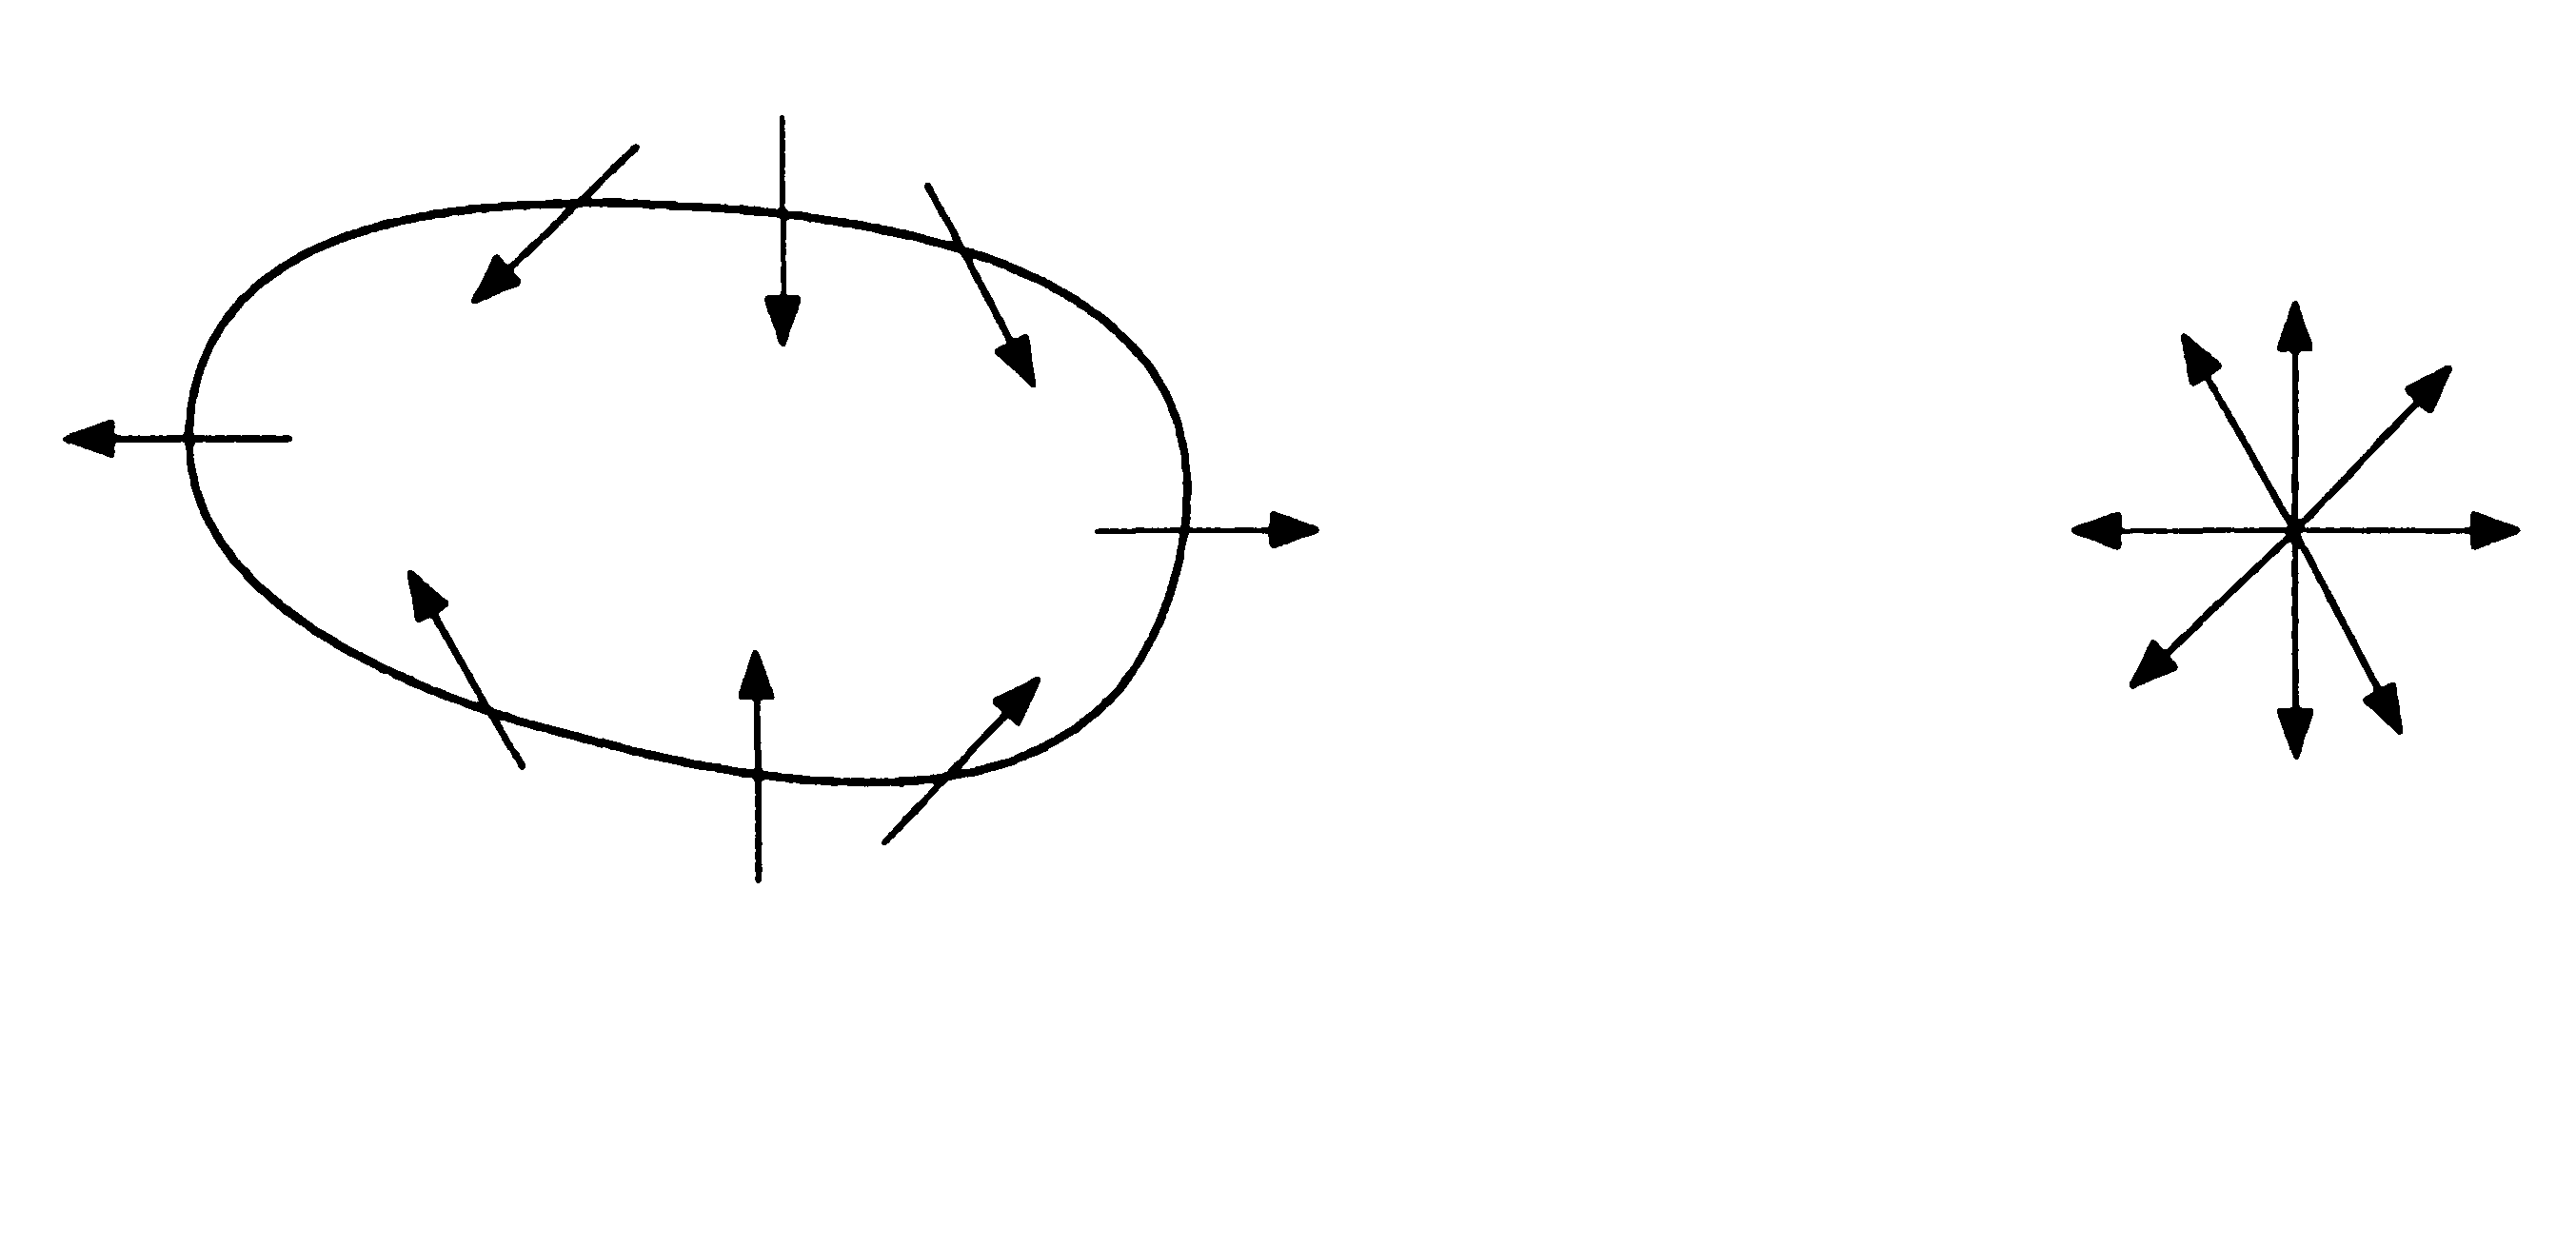
\includegraphics[width=0.82\textwidth]{images/Figures/figur-038.png}
\caption{Kapalı bir yörüngenin indeksinin $+1$ olması.}
\label{fig:6-8-4}
\end{figure}
\end{justify}

\subsection*{Örnek 6.8.1}
\addcontentsline{toc}{subsection}{Örnek 6.8.1}

\begin{justify}
Bir faz portresinde kapalı bir yörüngenin içinde yalnızca bir sabit nokta bulunduğu gözlensin. Bu sabit nokta eyer olabilir mi?

\textbf{Çözüm.} Hayır. Kapalı yörüngenin indeksi $+1$'dir. Eğer içindeki tek sabit nokta eyer olsaydı, bu noktanın indeksi $-1$ olurdu. İndekslerin toplanması kuralı $+1=-1$ gibi olanaksız bir sonuç vereceğinden, kapalı yörüngenin içinde tek başına eyer noktası bulunamaz. Tek sabit nokta varsa bu noktanın indeksi $+1$ olmalıdır; örneğin merkez, spiral ya da düğüm olabilir.

\begin{figure}[H]
\centering
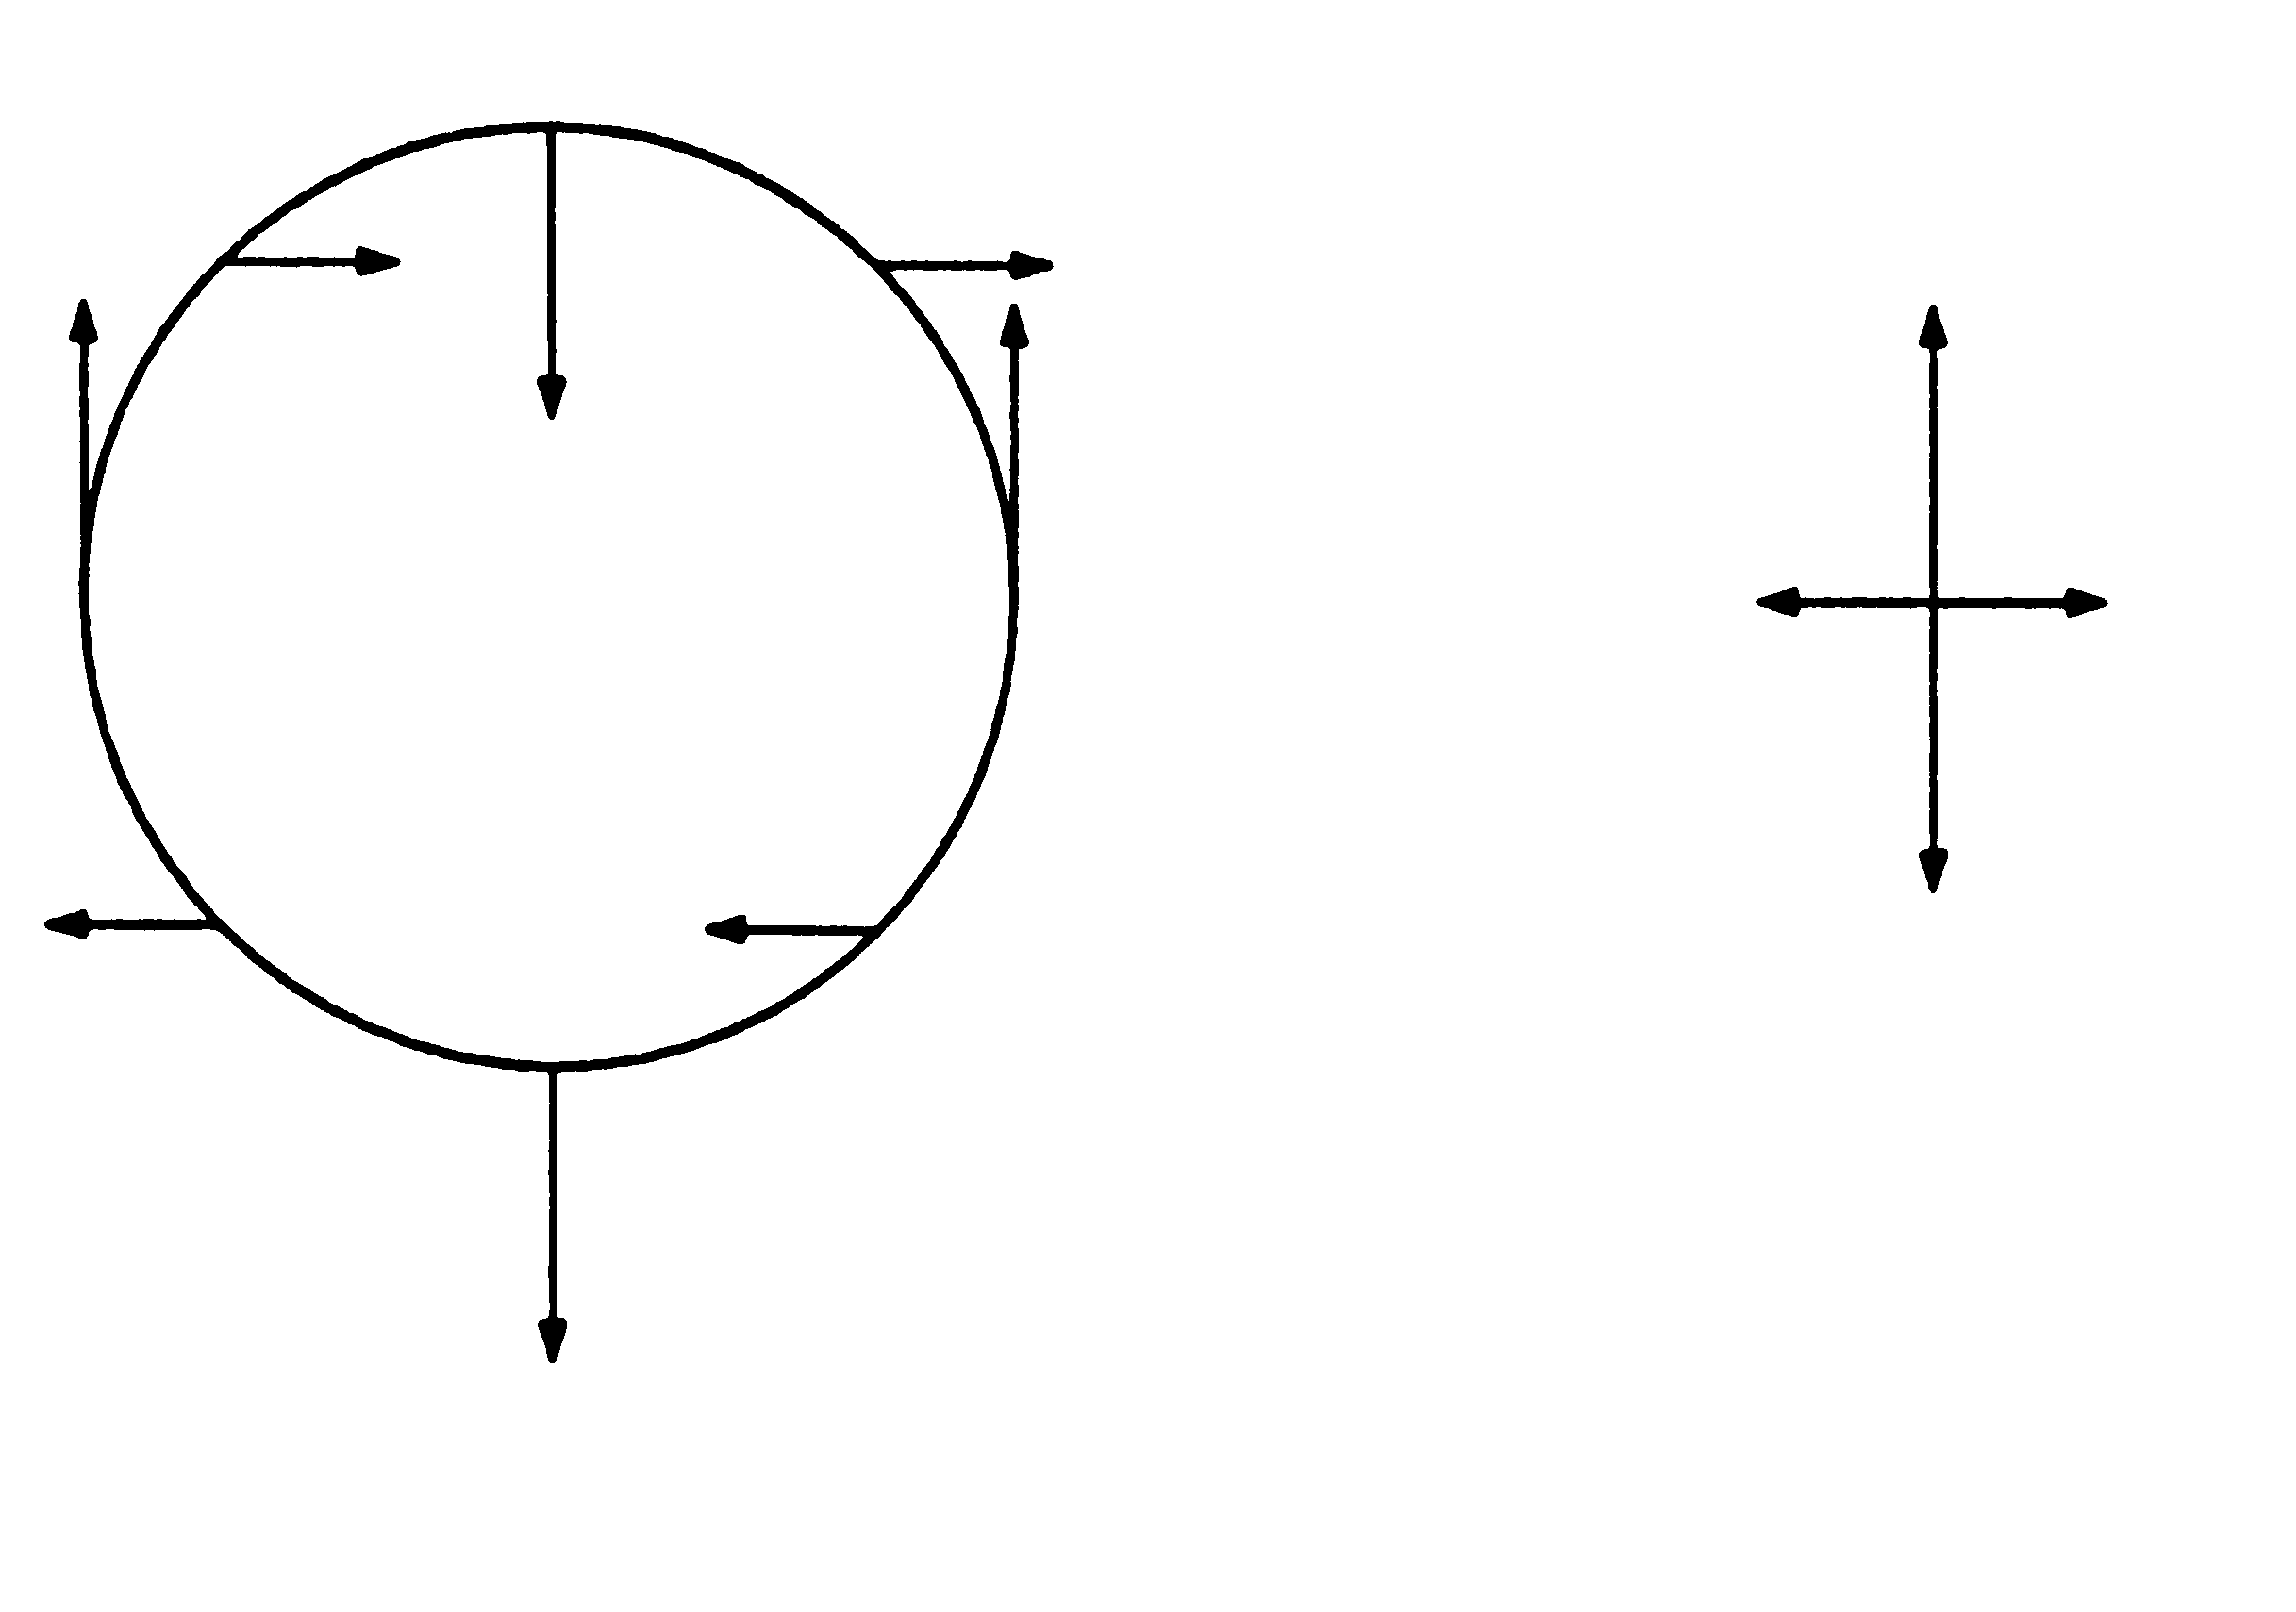
\includegraphics[width=0.82\textwidth]{images/Figures/figur-039.png}
\caption{Kapalı yörüngenin içinde tek başına eyer bulunamaması.}
\label{fig:6-8-5}
\end{figure}
\end{justify}

\subsection*{Örnek 6.8.2}
\addcontentsline{toc}{subsection}{Örnek 6.8.2}

\begin{justify}
Bir kapalı yörüngenin içinde iki eyer noktası varsa, içeride en az kaç tane eyer olmayan sabit nokta bulunmalıdır?

\textbf{Çözüm.} Kapalı yörüngenin indeksi $+1$'dir. İki eyerin toplam indeksi $-2$ olur. Eyer olmayan tipik hiperbolik sabit noktaların her biri $+1$ indeks taşır. Toplamın $+1$ olması için
\begin{equation}
-2+n=1
\end{equation}
olmalıdır. Buradan $n=3$ bulunur. Dolayısıyla içeride en az üç tane eyer olmayan sabit nokta bulunmalıdır.

\begin{figure}[H]
\centering
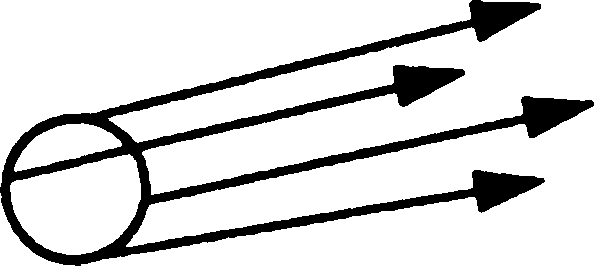
\includegraphics[width=0.82\textwidth]{images/Figures/figur-040.png}
\caption{İki eyer içeren kapalı yörüngede indeks dengesinin sağlanması.}
\label{fig:6-8-6}
\end{figure}
\end{justify}

\subsection*{Sınırlar ve Kullanım}
\addcontentsline{toc}{subsection}{Sınırlar ve Kullanım}

\begin{justify}
İndeks teorisi, faz portrelerinin mümkün olup olmadığını sınamak için güçlü ama kaba bir araçtır. İndeks yalnızca toplam topolojik bilgiyi verir; sabit noktaların tam konumlarını, yörüngelerin biçimini ya da kararlılık şiddetini belirlemez. Buna rağmen yanlış çizilmiş faz portrelerini yakalamakta çok etkilidir.

Örneğin bir kapalı yörüngenin içinde hiçbir sabit nokta çizilmemişse faz portresi eksiktir. Benzer biçimde, kapalı yörünge içinde yalnızca iki eyer noktası çizilmişse toplam indeks $-2$ olur ve bu da kapalı yörüngenin indeksi olan $+1$ ile çelişir. Bu tür denetimler özellikle karmaşık doğrusal olmayan sistemlerde faz portresinin tutarlılığını kontrol etmek için kullanılır.

\begin{figure}[H]
\centering
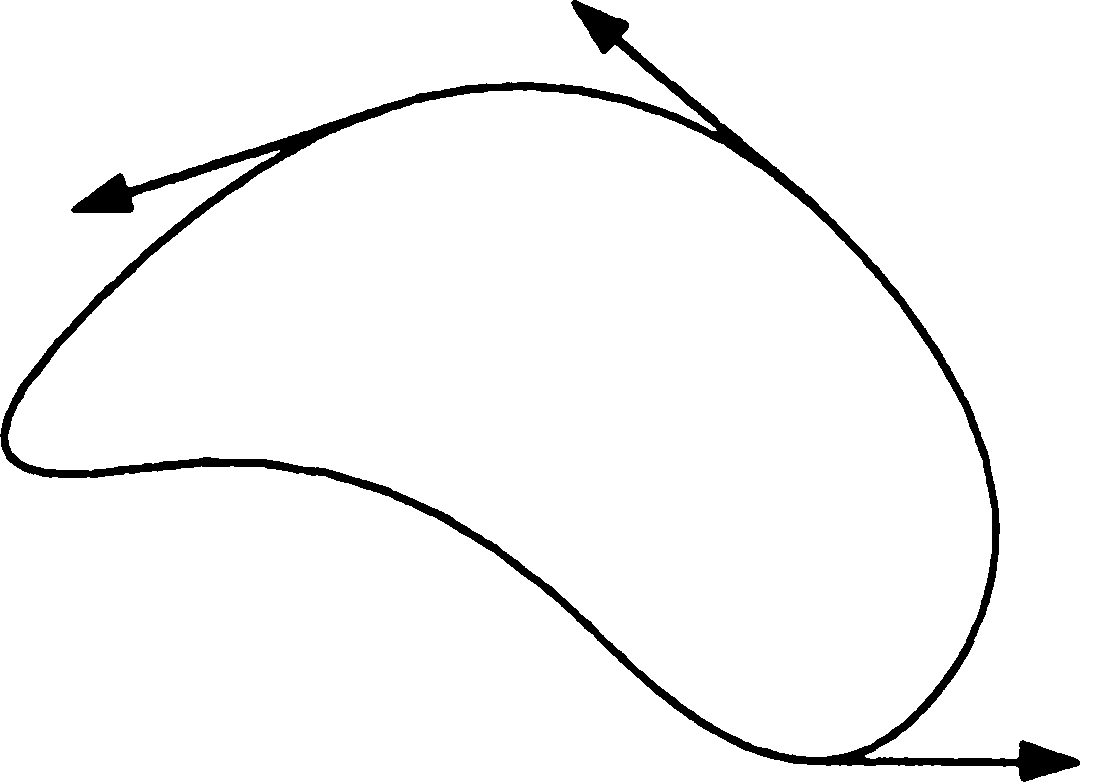
\includegraphics[width=0.82\textwidth]{images/Figures/figur-041.png}
\caption{İndeks kuralıyla elenen tutarsız faz portresi örnekleri.}
\label{fig:6-8-7}
\end{figure}

Sonuç olarak indeks teorisi, yerel sabit nokta analizini küresel faz portresi bilgisiyle birleştirir. Düğüm, spiral, merkez ve eyer gibi yerel yapıların kapalı eğriler içinde nasıl dengelenmesi gerektiğini gösterir.

\begin{figure}[H]
\centering
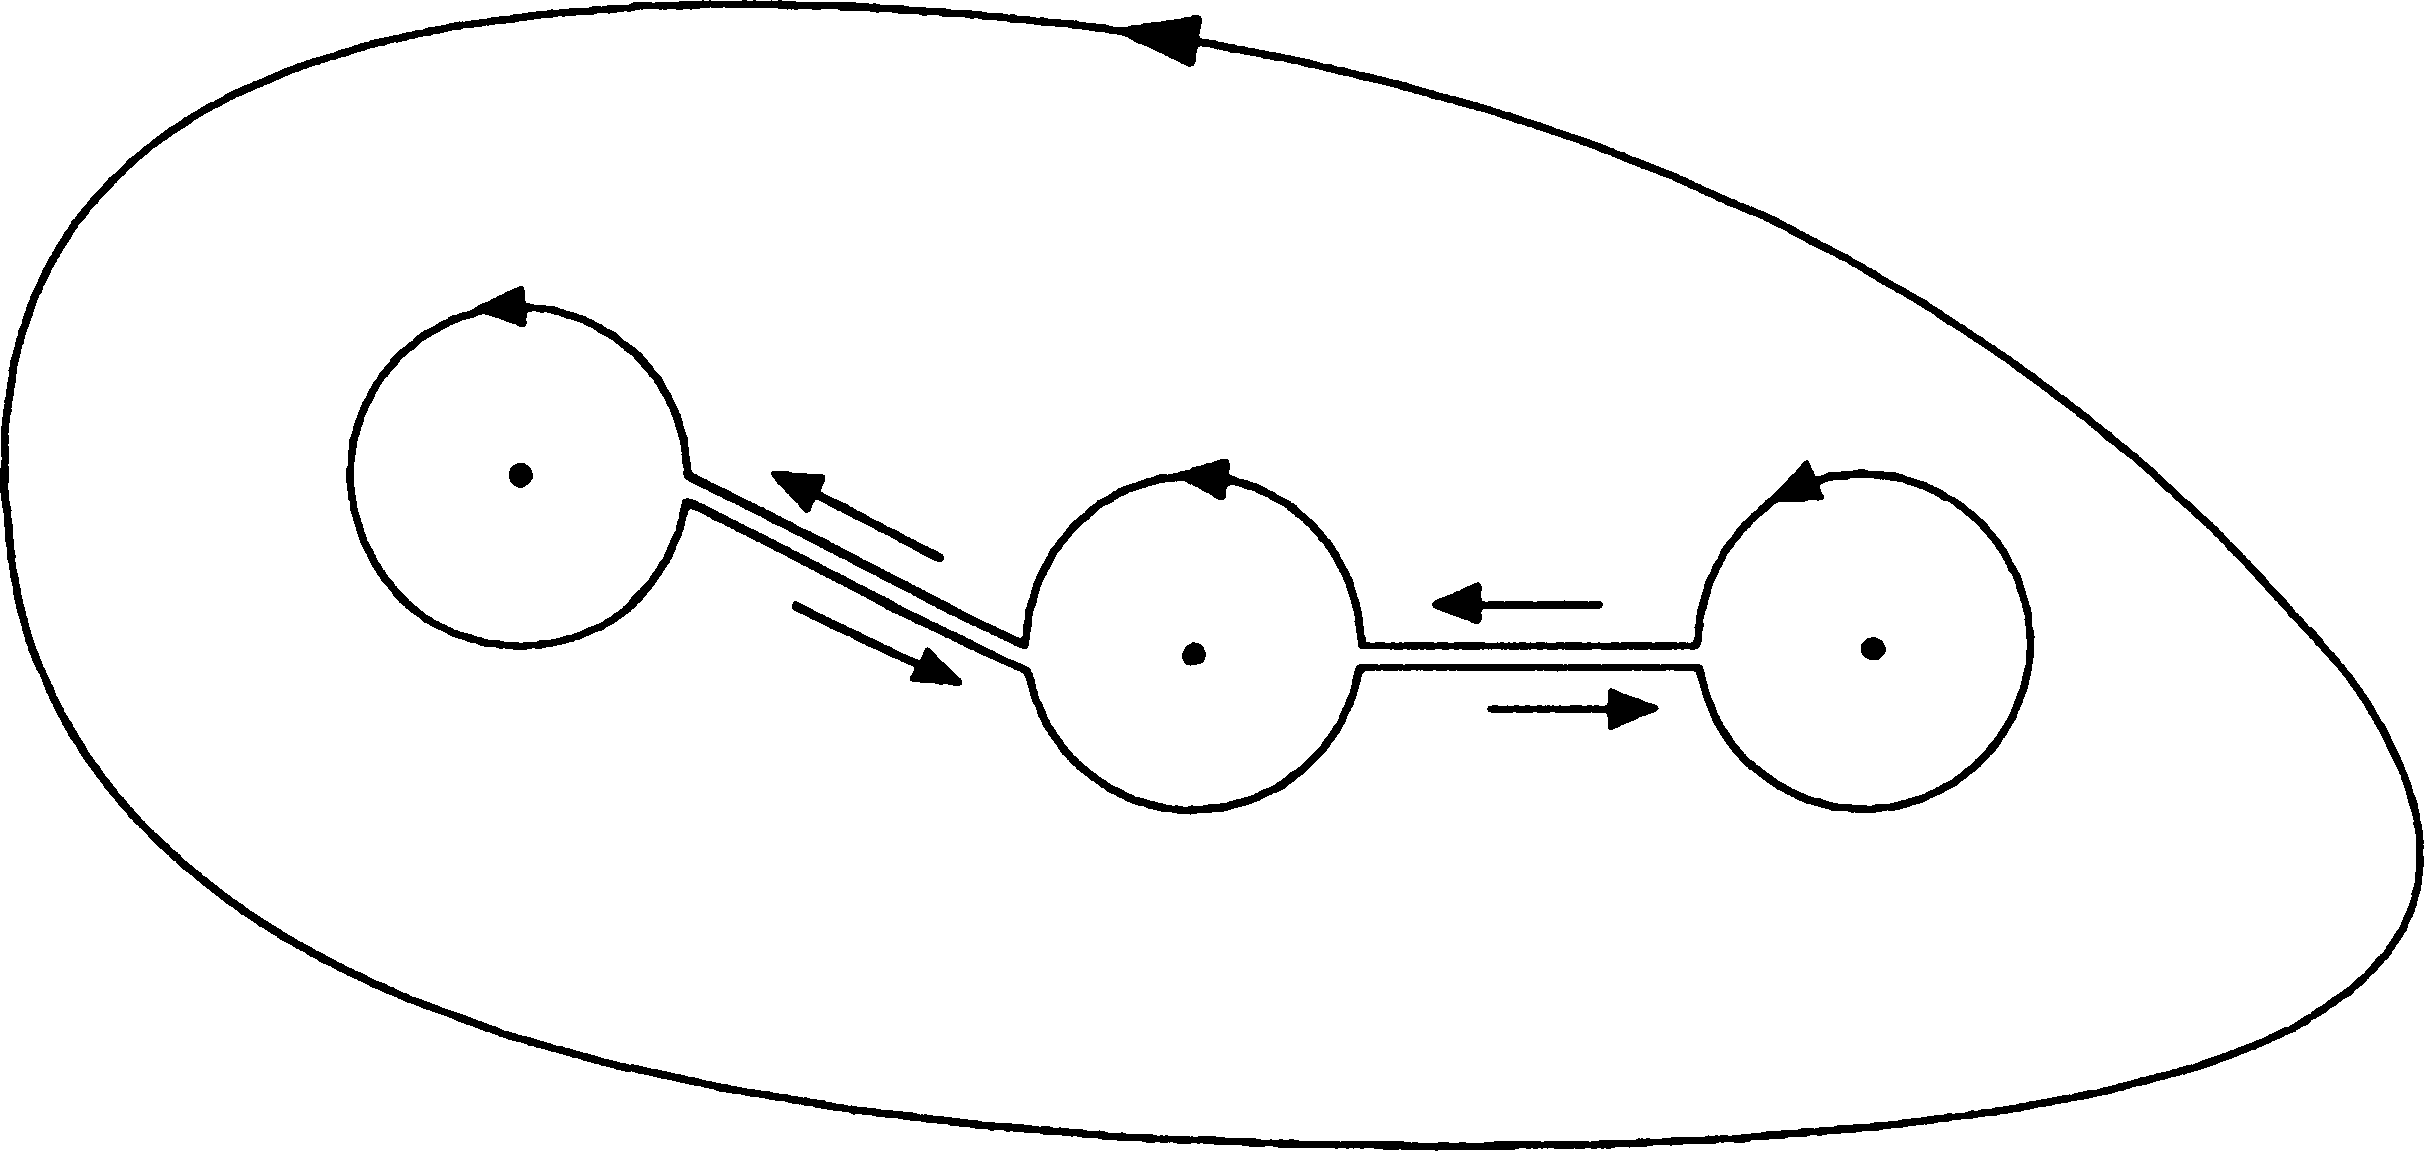
\includegraphics[width=0.82\textwidth]{images/Figures/figur-042.png}
\caption{Yerel sabit nokta indekslerinin küresel faz portresiyle uyumu.}
\label{fig:6-8-8}
\end{figure}
\begin{figure}[H]
\centering
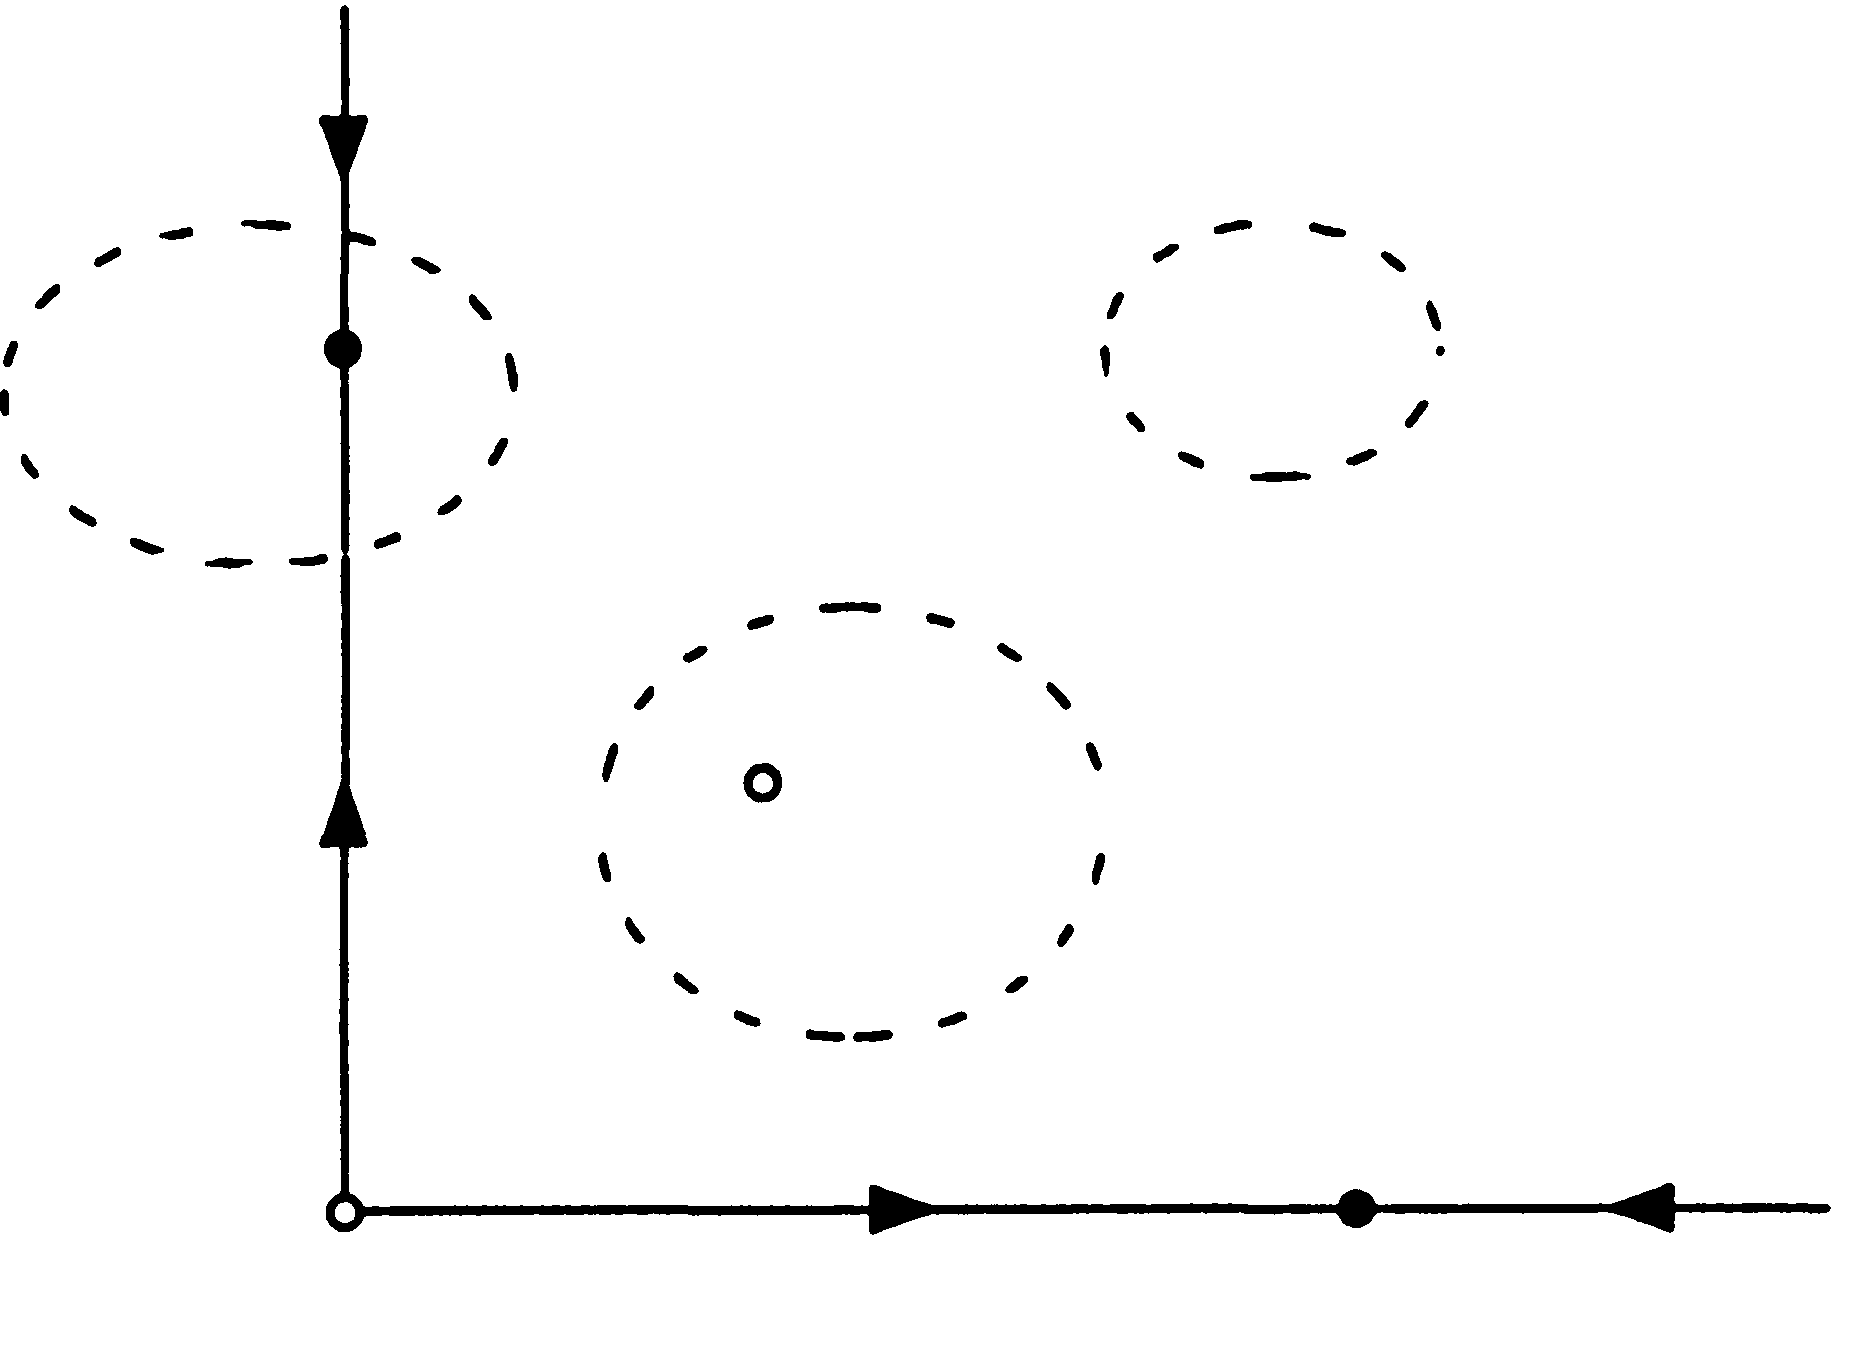
\includegraphics[width=0.82\textwidth]{images/Figures/figur-043.png}
\caption{İndeks teorisiyle faz portresi tutarlılığının özet gösterimi.}
\label{fig:6-8-9}
\end{figure}
\end{justify}
\chapter*{Alıştırmalar ve Çözümleri}
\phantomsection
\addcontentsline{toc}{chapter}{Alıştırmalar ve Çözümleri}

\begin{justify}
Bu bölümde, Faz Düzlemi bölümünün ana başlıklarına göre düzenlenmiş alıştırmalar ve kısa çözümleri verilmiştir. Sorular, ilgili alt bölümdeki temel kavramları pekiştirmek amacıyla hazırlanmıştır.
\end{justify}

\phantomsection
\section*{6.1 Faz Portreleri}
\addcontentsline{toc}{section}{6.1 Faz Portreleri}

\phantomsection
\subsection*{Alıştırma 6.1.1}
\addcontentsline{toc}{subsection}{Alıştırma 6.1.1}

\begin{justify}
Aşağıdaki sistemin sabit noktalarını bulun:
\begin{align}
\dot{x} &= y,\\
\dot{y} &= x-x^3.
\end{align}

\textbf{Çözüm.} Sabit noktalarda $\dot{x}=0$ ve $\dot{y}=0$ olmalıdır. İlk denklemden $y=0$ bulunur. İkinci denklemden
\begin{equation}
x-x^3=x(1-x^2)=0
\end{equation}
olur. Dolayısıyla $x=0$, $x=1$ veya $x=-1$ bulunur. Sabit noktalar
\begin{equation}
(-1,0),\quad (0,0),\quad (1,0)
\end{equation}
şeklindedir.
\end{justify}

\phantomsection
\subsection*{Alıştırma 6.1.2}
\addcontentsline{toc}{subsection}{Alıştırma 6.1.2}

\begin{justify}
Aşağıdaki sistem için $x$-nullcline ve $y$-nullcline eğrilerini bulun:
\begin{align}
\dot{x} &= x(1-y),\\
\dot{y} &= y(x-2).
\end{align}

\textbf{Çözüm.} $x$-nullcline, $\dot{x}=0$ koşulunu sağlayan noktalar kümesidir. Buradan
\begin{equation}
x(1-y)=0
\end{equation}
olduğundan $x=0$ veya $y=1$ elde edilir. $y$-nullcline için $\dot{y}=0$ yazılır:
\begin{equation}
y(x-2)=0.
\end{equation}
Dolayısıyla $y=0$ veya $x=2$ bulunur. Nullcline kesişimleri sabit noktaları verir: $(0,0)$ ve $(2,1)$.
\end{justify}

\phantomsection
\section*{6.2 Doğrusal Sistemler ve Lineerleştirme}
\addcontentsline{toc}{section}{6.2 Doğrusal Sistemler ve Lineerleştirme}

\phantomsection
\subsection*{Alıştırma 6.2.1}
\addcontentsline{toc}{subsection}{Alıştırma 6.2.1}

\begin{justify}
Aşağıdaki sistemin orijindeki sabit noktasını sınıflandırın:
\begin{align}
\dot{x} &= 2x+y,\\
\dot{y} &= x+2y.
\end{align}

\textbf{Çözüm.} Matris
\begin{equation}
A=\begin{pmatrix}2&1\\1&2\end{pmatrix}
\end{equation}
şeklindedir. Karakteristik denklem
\begin{equation}
\det(A-\lambda I)=(2-\lambda)^2-1=0
\end{equation}
olur. Buradan $\lambda_1=3$ ve $\lambda_2=1$ bulunur. Her iki özdeğer de pozitif ve gerçektir. Bu nedenle orijin kararsız düğümdür.
\end{justify}

\phantomsection
\subsection*{Alıştırma 6.2.2}
\addcontentsline{toc}{subsection}{Alıştırma 6.2.2}

\begin{justify}
Aşağıdaki doğrusal olmayan sistemin orijin yakınındaki davranışını lineerleştirme ile belirleyin:
\begin{align}
\dot{x} &= -x-y+x^2,\\
\dot{y} &= x-y+y^3.
\end{align}

\textbf{Çözüm.} Jacobian matrisi
\begin{equation}
J(x,y)=\begin{pmatrix}-1+2x&-1\\1&-1+3y^2\end{pmatrix}
\end{equation}
olur. Orijinde
\begin{equation}
A=J(0,0)=\begin{pmatrix}-1&-1\\1&-1\end{pmatrix}
\end{equation}
bulunur. İz $\tau=-2$, determinant $\Delta=2$ ve diskriminant $\tau^2-4\Delta=-4<0$'dır. Özdeğerlerin reel kısmı negatiftir. Bu nedenle orijin kararlı spiraldir.
\end{justify}

\phantomsection
\section*{6.3 Varoluş, Teklik ve Topolojik Sonuçlar}
\addcontentsline{toc}{section}{6.3 Varoluş, Teklik ve Topolojik Sonuçlar}

\phantomsection
\subsection*{Alıştırma 6.3.1}
\addcontentsline{toc}{subsection}{Alıştırma 6.3.1}

\begin{justify}
Düzgün bir vektör alanında iki farklı yörüngenin aynı noktadan geçemeyeceğini açıklayın.

\textbf{Çözüm.} Düzgün bir vektör alanında başlangıç değer problemi yerel olarak tek çözüme sahiptir. Eğer iki farklı yörünge aynı $\mathbf{x}_0$ noktasından geçseydi, bu noktayı başlangıç koşulu alan iki farklı çözüm elde edilmiş olurdu. Bu durum teklik teoremiyle çelişir. Dolayısıyla faz düzleminde yörüngeler birbirini kesemez; yalnızca aynı yörüngenin farklı zamanlardaki gösterimleri çakışabilir.
\end{justify}

\phantomsection
\subsection*{Alıştırma 6.3.2}
\addcontentsline{toc}{subsection}{Alıştırma 6.3.2}

\begin{justify}
Bir yörüngenin kapalı bir eğri oluşturduğunu varsayalım. Bu yörünge üzerinde sabit nokta bulunabilir mi?

\textbf{Çözüm.} Hayır. Kapalı yörünge üzerinde hareket eden faz noktası için vektör alanı sıfırdan farklı olmalıdır; aksi hâlde faz noktası sabit noktada durur ve yörünge ilerleyemez. Sabit noktada $\dot{x}=\dot{y}=0$ olduğundan çözüm zamana göre sabittir. Teklik nedeniyle aynı başlangıç noktasından hem sabit çözüm hem de kapalı yörünge çözümü çıkamaz.
\end{justify}

\phantomsection
\section*{6.4 Limit Çevrimler}
\addcontentsline{toc}{section}{6.4 Limit Çevrimler}

\phantomsection
\subsection*{Alıştırma 6.4.1}
\addcontentsline{toc}{subsection}{Alıştırma 6.4.1}

\begin{justify}
Kutupsal koordinatlarda verilen
\begin{align}
\dot{r} &= r(1-r),\\
\dot{\theta} &= 1
\end{align}
sisteminin limit çevrimini bulun ve kararlılığını belirleyin.

\textbf{Çözüm.} Radyal denklem $\dot{r}=r(1-r)$ şeklindedir. Sabit yarıçaplar $r=0$ ve $r=1$'dir. $0<r<1$ için $\dot{r}>0$, $r>1$ için $\dot{r}<0$ olur. Bu nedenle yörüngeler $r=1$ çemberine yaklaşır. $r=1$ kararlı limit çevrimdir. $\dot{\theta}=1$ olduğundan hareket saat yönünün tersinedir.
\end{justify}

\phantomsection
\subsection*{Alıştırma 6.4.2}
\addcontentsline{toc}{subsection}{Alıştırma 6.4.2}

\begin{justify}
Kutupsal koordinatlarda
\begin{align}
\dot{r} &= r(r-1),\\
\dot{\theta} &= 1
\end{align}
sistemi için $r=1$ çevriminin kararlılığını inceleyin.

\textbf{Çözüm.} $0<r<1$ için $r-1<0$ olduğundan $\dot{r}<0$ ve yörüngeler orijine doğru gider. $r>1$ için $\dot{r}>0$ olduğundan yörüngeler dışarı doğru uzaklaşır. Dolayısıyla $r=1$ çevrimi kararsız limit çevrimdir. Çevrimin biraz içindeki ve biraz dışındaki yörüngeler çevrimden uzaklaşır.
\end{justify}

\phantomsection
\section*{6.5 Korunumlu Sistemler}
\addcontentsline{toc}{section}{6.5 Korunumlu Sistemler}

\phantomsection
\subsection*{Alıştırma 6.5.1}
\addcontentsline{toc}{subsection}{Alıştırma 6.5.1}

\begin{justify}
Aşağıdaki sistem için korunan enerji fonksiyonunu bulun:
\begin{align}
\dot{x} &= y,\\
\dot{y} &= -x-x^3.
\end{align}

\textbf{Çözüm.} Sistem $\ddot{x}=-x-x^3$ biçiminde yazılabilir. Bu denklem
\begin{equation}
\ddot{x}+\frac{dV}{dx}=0
\end{equation}
formundadır. Buradan
\begin{equation}
\frac{dV}{dx}=x+x^3
\end{equation}
olur. İntegral alınırsa
\begin{equation}
V(x)=\frac{1}{2}x^2+\frac{1}{4}x^4
\end{equation}
bulunur. Dolayısıyla korunan enerji
\begin{equation}
E(x,y)=\frac{1}{2}y^2+\frac{1}{2}x^2+\frac{1}{4}x^4
\end{equation}
şeklindedir.
\end{justify}

\phantomsection
\subsection*{Alıştırma 6.5.2}
\addcontentsline{toc}{subsection}{Alıştırma 6.5.2}

\begin{justify}
Korunumlu bir sistemde asimptotik kararlı sabit nokta bulunamayacağını enerji yorumu ile açıklayın.

\textbf{Çözüm.} Korunumlu sistemde enerji yörünge boyunca sabittir. Asimptotik kararlı bir sabit nokta olsaydı, yakınındaki birçok farklı başlangıç koşulu zamanla bu noktaya yaklaşırdı. Bu durumda bu farklı başlangıç koşullarının enerjileri, limitte sabit noktanın enerjisine eşit olmak zorunda kalırdı. Fakat enerji başlangıçtan itibaren değişmediği için bütün bu noktaların aynı enerji seviyesinde bulunması gerekir. Açık bir komşulukta enerji sabit olamayacağından asimptotik kararlılık mümkün değildir.
\end{justify}

\phantomsection
\section*{6.6 Tersinir Sistemler}
\addcontentsline{toc}{section}{6.6 Tersinir Sistemler}

\phantomsection
\subsection*{Alıştırma 6.6.1}
\addcontentsline{toc}{subsection}{Alıştırma 6.6.1}

\begin{justify}
Aşağıdaki sistemin $t\mapsto -t$, $y\mapsto -y$ dönüşümü altında tersinir olduğunu gösterin:
\begin{align}
\dot{x} &= y+x^2y,\\
\dot{y} &= -x+y^2.
\end{align}

\textbf{Çözüm.} Bu dönüşüm altında $x$ değişmez, $y$ işaret değiştirir ve zaman ters çevrilir. Tersinirlik için $\dot{x}$ denkleminin $y$'ye göre tek, $\dot{y}$ denkleminin ise $y$'ye göre çift olması gerekir. Burada
\begin{equation}
y+x^2y
\end{equation}
$y$'ye göre tek fonksiyondur. Ayrıca
\begin{equation}
-x+y^2
\end{equation}
$y$'ye göre çift fonksiyondur. Bu nedenle sistem verilen dönüşüm altında tersinirdir.
\end{justify}

\phantomsection
\subsection*{Alıştırma 6.6.2}
\addcontentsline{toc}{subsection}{Alıştırma 6.6.2}

\begin{justify}
Tersinir bir sistemde $x$ eksenini iki farklı noktada kesen ve bu kesişimlerde vektör alanına teğet olmayan bir yörüngenin neden kapalı olduğunu açıklayın.

\textbf{Çözüm.} $x$ ekseni simetri doğrusu olsun. Yörünge $x$ eksenini iki noktada keserse, bu iki kesişim arasında kalan yörünge parçası simetri dönüşümüyle eksenin diğer tarafına yansıtılabilir. Zaman da ters çevrildiği için yansıtılmış parça aynı diferansiyel denklemin çözümü olur; fakat ok yönü tersine döner. Teklik nedeniyle bu yansıtılmış parça, ilk parçayı tamamlayan yörüngedir. Böylece iki parça birleşerek kapalı bir eğri oluşturur.
\end{justify}

\phantomsection
\section*{6.7 Sarkaç}
\addcontentsline{toc}{section}{6.7 Sarkaç}

\phantomsection
\subsection*{Alıştırma 6.7.1}
\addcontentsline{toc}{subsection}{Alıştırma 6.7.1}

\begin{justify}
Boyutsuz sönümsüz sarkaç
\begin{equation}
\ddot{\theta}+\sin\theta=0
\end{equation}
için enerji fonksiyonunu bulun.

\textbf{Çözüm.} Denklemi $\dot{\theta}$ ile çarpalım:
\begin{equation}
\dot{\theta}\ddot{\theta}+\dot{\theta}\sin\theta=0.
\end{equation}
İlk terim $\frac{d}{dt}(\frac{1}{2}\dot{\theta}^{2})$, ikinci terim ise $\frac{d}{dt}(-\cos\theta)$ biçimindedir. Dolayısıyla
\begin{equation}
E(\theta,\dot{\theta})=\frac{1}{2}\dot{\theta}^{2}-\cos\theta
\end{equation}
korunan enerji fonksiyonudur.
\end{justify}

\phantomsection
\subsection*{Alıştırma 6.7.2}
\addcontentsline{toc}{subsection}{Alıştırma 6.7.2}

\begin{justify}
Sönümsüz sarkaçta $(0,0)$ ve $(\pi,0)$ sabit noktalarını sınıflandırın.

\textbf{Çözüm.} Faz düzlemi sistemi
\begin{align}
\dot{\theta} &= v,\\
\dot{v} &= -\sin\theta
\end{align}
şeklindedir. Jacobian
\begin{equation}
J(\theta,v)=\begin{pmatrix}0&1\\-\cos\theta&0\end{pmatrix}
\end{equation}
olur. $(0,0)$ noktasında
\begin{equation}
J(0,0)=\begin{pmatrix}0&1\\-1&0\end{pmatrix}
\end{equation}
ve özdeğerler $\lambda=\pm i$'dir. Enerji minimumu nedeniyle bu nokta doğrusal olmayan merkezdir. $(\pi,0)$ noktasında
\begin{equation}
J(\pi,0)=\begin{pmatrix}0&1\\1&0\end{pmatrix}
\end{equation}
ve özdeğerler $\lambda=\pm1$'dir. Bu nedenle $(\pi,0)$ eyer noktasıdır.
\end{justify}

\phantomsection
\section*{6.8 İndeks Teorisi}
\addcontentsline{toc}{section}{6.8 İndeks Teorisi}

\phantomsection
\subsection*{Alıştırma 6.8.1}
\addcontentsline{toc}{subsection}{Alıştırma 6.8.1}

\begin{justify}
Bir kapalı yörüngenin içinde yalnızca iki sabit nokta olduğunu varsayın. Bunlardan biri eyer noktasıysa, diğerinin indeksi ne olmalıdır?

\textbf{Çözüm.} Kapalı yörüngenin indeksi $+1$'dir. Eyer noktasının indeksi $-1$ olduğundan diğer sabit noktanın indeksi $I$ için
\begin{equation}
-1+I=1
\end{equation}
olmalıdır. Buradan $I=2$ bulunur. Bu nedenle diğer sabit nokta sıradan hiperbolik düğüm, spiral veya merkez olamaz; çünkü onların indeksleri $+1$'dir. Böyle bir faz portresi ancak dejenereliği olan daha özel bir sabit nokta ile mümkün olabilir.
\end{justify}

\phantomsection
\subsection*{Alıştırma 6.8.2}
\addcontentsline{toc}{subsection}{Alıştırma 6.8.2}

\begin{justify}
Bir kapalı eğrinin içinde iki merkez ve üç eyer noktası varsa, eğrinin indeksi kaçtır?

\textbf{Çözüm.} Merkezlerin her birinin indeksi $+1$, eyerlerin her birinin indeksi $-1$'dir. Toplam indeks
\begin{equation}
I_C=2(+1)+3(-1)=-1
\end{equation}
olur. Dolayısıyla kapalı eğrinin indeksi $-1$'dir. Eğer bu eğri bir kapalı yörünge olsaydı indeksi $+1$ olmak zorunda kalırdı; bu nedenle verilen sabit nokta düzeni tek başına bir kapalı yörüngenin içinde bulunamaz.
\end{justify}

\newpage

\chapter*{Sonuç}
\phantomsection
\addcontentsline{toc}{chapter}{Sonuç}

\begin{justify}
Bu çalışmanın mevcut sürümünde Strogatz kitabının 6.1 numaralı kısmı Türkçeye çevrilmiş ve sadeleştirilmiş tez formatına yerleştirilmiştir. Sonraki aşamada 6. bölümün kalan kısımları ve bölüm sonu sorularının ayrıntılı çözümleri eklenecektir.
\end{justify}

\newpage

\begin{thebibliography}{1}

\bibitem{strogatz}
Steven H. Strogatz, \textit{Nonlinear Dynamics and Chaos}, Bölüm 6: Phase Plane, kaynak PDF: \textit{Strogatz Book-Bölüm-6.pdf}.

\end{thebibliography} 


\end{document}
